\documentclass{ieeeaccess}
\usepackage{cite}
\usepackage{amsmath,amssymb,amsfonts}
\usepackage{algorithmic}
\usepackage{graphicx}
\usepackage{textcomp}
\usepackage{booktabs}
\usepackage{multirow}
\usepackage{subcaption}
\usepackage{bm}
\usepackage{float}
\makeatletter
\AtBeginDocument{\DeclareMathVersion{bold}
\SetSymbolFont{operators}{bold}{T1}{times}{b}{n}
\SetSymbolFont{NewLetters}{bold}{T1}{times}{b}{it}
\SetMathAlphabet{\mathrm}{bold}{T1}{times}{b}{n}
\SetMathAlphabet{\mathit}{bold}{T1}{times}{b}{it}
\SetMathAlphabet{\mathbf}{bold}{T1}{times}{b}{n}
\SetMathAlphabet{\mathtt}{bold}{OT1}{pcr}{b}{n}
\SetSymbolFont{symbols}{bold}{OMS}{cmsy}{b}{n}
\renewcommand\boldmath{\@nomath\boldmath\mathversion{bold}}}
\makeatother

\def\BibTeX{{\rm B\kern-.05em{\sc i\kern-.025em b}\kern-.08em
    T\kern-.1667em\lower.7ex\hbox{E}\kern-.125emX}}

%Your document starts from here ___________________________________________________
\begin{document}


\title{Design and Evaluation of Multi-Agent Architectures
for Stock Price Prediction: A Vietnam Case Study}
\author{
    \uppercase{Duong Nguyen Minh}\authorrefmark{1}, 
    \uppercase{Dat Nguyen Huu}\authorrefmark{2}
}

\address[1]{School of Computing, Phenikaa University, Vietnam\\
(e-mail: 23010441@st.phenikaa-uni.edu.vn)}

\address[2]{School of Computing, Phenikaa University, Vietnam\\
(e-mail: dat.nguyenhuu@phenikaa-uni.edu.vn)}


\tfootnote{This paragraph of the first footnote will contain support
information, including sponsor and financial support acknowledgment. For
example, ``This work was supported in part by the U.S. Department of
Commerce under Grant BS123456.''}

\markboth
{Author \headeretal: Preparation of Papers for IEEE TRANSACTIONS and JOURNALS}
{Author \headeretal: Preparation of Papers for IEEE TRANSACTIONS and JOURNALS}

\corresp{Corresponding author: Dat Nguyen Huu (e-mail: dat.nguyenhuu@phenikaa-uni.edu.vn). Code and data are available at: \url{https://github.com/nminduo2k5/Multi-agentVNstock.git}}


\begin{abstract}
Traditional stock price prediction methods struggle in emerging markets characterized by retail investor dominance, high volatility, and sentiment-driven trading. We address this gap by developing a multi-agent framework tailored to Vietnam's unique market structure, where 85-90\% of participants are retail investors operating under a T+2.5 settlement cycle. Our system integrates six specialized agents analyzing technical indicators, fundamental metrics, risk profiles, news sentiment, macroeconomic signals, and market microstructure through three coordination mechanisms: Hierarchical, Round Robin, and Ensemble Voting. Evaluated on four representative Vietnamese stocks across 3-day, 14-day, and 60-day horizons, Ensemble Voting achieves consistently superior medium-term performance with MAPE ranging from 1.6\% to 10.0\%, outperforming traditional LSTM baselines by 25-40\% and single-agent approaches by 15-30\%. The framework's interpretable architecture supports regulatory assessment and tactical investment decision-making in retail-dominated markets, with broader implications for emerging financial systems.

\end{abstract}

\begin{keywords}
Architectures, Multi-agent, Price Prediction,Vietnam Stock
\end{keywords}

\titlepgskip=-21pt

\maketitle

\section{Introduction}
\label{sec:introduction}
The fast growth of digital technology in equity markets and the increasing availability of real-time market data  have created new opportunities for using artificial intelligence (AI) in trading and investment analysis. In Vietnam’s stock market, this change is especially relevant. By the end of 2024, there were about 9.3 million accounts for trading securities, with 99\% owned by domestic investors. Retail investors made up more than 80\% of all trade value \cite{vietnamnews2025}. These numbers show that Vietnam’s market is heavily driven by retail investors. It also shows that the market has high volatility, some inefficiencies, and a regulatory system that is still changing.

Traditional methods of equity-market analysis—technical analysis based on price patterns and fundamental analysis rooted in corporate disclosures—often struggle to capture the complex, non-linear relationships found in emerging markets. For instance, empirical evidence from Vietnam has revealed sluggish information dissemination, intraday trading frictions, and pronounced influences from investor sentiment and speculative behavior \cite{ha2025}. These characteristics underscore the limitations of conventional modelling approaches and reinforce the necessity for more adaptive and robust analytical frameworks.

Using deep learning setups with multi-agent systems presents a promising new way to deal with these challenges. Deep learning models can automatically extract informative representations from large and complex datasets, thereby uncovering latent patterns and improving predictive accuracy. At the same time, multi-agent system designs let us simulate different market players and how they interact, offering a more realistic depiction of how markets work and how investors act.

To properly utilize AI-based strategies within Vietnam's stock market, it's essential to customize them carefully to align with its specific operational and conduct aspects. The primary issues include data that is either disorganised or deficient, market behavior predominantly swayed by the sentiments of retail investors, and a legal and supervisory environment that constantly evolves and diverges from that of more mature economic systems. Therefore, combining complex analysis approaches with the unique features of the Vietnamese market is indispensable for unlocking the full potential of AI within this domain.

Accordingly, this study proposes a tailored simulation framework that combines specialised agent-modules and architectural designs to model Vietnamese stock-market dynamics. The focus will be on testing trading strategies, liquidity and volatility responses, and inter-agent communication under different coordination architectures. By doing so, the research contributes both to the academic understanding of agent-to-agent interactions in emerging markets and to the practical design of decision-support tools for Vietnam’s financial ecosystem.



\section{Literature Review}
\label{sec:Literature Review}

\subsection{Stock Market Data}
Data from worldwide stock exchanges has been acknowledged for a considerable period as a vital element for scholarly investigations and choices made by organizations. Established trading platforms like the NYSE, NASDAQ, LSE, and TSE function on a substantial level, having market values that go beyond USD 40–50 trillion when added up, and regular intraday trading volumes frequently go beyond hundreds of billions each day \cite{WorldFederation2024}. These marketplaces offer revisions to order books at the millisecond level, comprehensive limit order details (Level 3), and uniform high-frequency data streams appropriate for automated trading systems and studies into execution at the microsecond level \cite{Jones2019HFT}. These kinds of frameworks have paved the way for detailed studies of the structure of markets, latency-based arbitrage strategies, and how systemic risks extend throughout high-frequency settings.

In comparison, the stock market of Vietnam, which includes HOSE, HNX, and UPCoM, remains structurally smaller and data-constrained. The total value of all listed companies in 2024 is about USD 250–300 billion \cite{HOSE2024Report}, and the average value of daily trades is between USD 800 million and 1.2 billion, significantly lower than regional peers such as Thailand and Malaysia \cite{ADB2024}. Also, the data that is available is limited to the highest, lowest, opening, and closing prices at the end of the day, a summary of order flow, and recently, some limited visibility of the order book, but it does not have timestamps measured in microseconds or complete insight into the depth of orders \cite{Nguyen2022Microstructure}. These limitations in structure show the general traits of markets that are still developing, which include bigger swings in returns, less involvement from big institutions, and more reaction to changes in rules and laws.

A key behavioral divergence arises from the dominance of retail investors, who account for more than 85\% of total trading volume in Vietnam \cite{SSI2024Retail}. In contrast to markets run by big organizations where prices usually change based on news and profits, price changes in Vietnam tend to be more affected by government instructions, unofficial means of communication, and guesses based on feelings \cite{StateBank2023}. While markets around the world are starting to use news chosen by AI and different kinds of data in their trading systems \cite{BloombergAI2023}, what happens in the Vietnamese market is often influenced by what people feel on social media locally and what they think will happen with major government policies.

In conclusion, The Vietnam stock market is not just a basic example of worldwide marketplaces; instead, it is a complex, emotionally reactive environment with a wide variety of behaviors, functioning with limited information, changing rules, and strong involvement from individual investors. This unique arrangement turns it into a fascinating place to test how well agent-based models and flexible AI systems work in developing economies.

\subsection{AI in Stock Price Prediction}

Over recent decades, artificial intelligence has advanced significantly in stock price prediction. Early studies focused on machine learning methods such as support vector machines, decision trees, random forests, and artificial neural networks, which captured non-linear relations between financial variables and returns and often outperformed statistical approaches \cite{kim2003,huang2005,patel2015}. Deep learning models like recurrent neural networks and long short-term memory further improved temporal analysis of financial time series \cite{fischer2018,chen2015}.

More recently, research has shifted toward \textit{Multi-Agent Systems} (MAS), where agents interact in simulated markets. Unlike traditional models treating prices as isolated data streams, MAS capture dynamic relations among traders, brokers, and regulators, enabling the study of phenomena such as herd behavior, bubbles, or irregularities \cite{lebaron2006,chen2012}. Combining reinforcement learning with agent-based simulations also deepens analysis of trading strategies, market stability, and inter-agent communication \cite{tesfatsion2006,wang2021}.

While the majority of MAS-based financial research has focused on mature markets such as the U.S. and China, empirical applications to emerging markets remain notably scarce. Regarding Vietnam, the AI-driven research currently available is mainly about price predictor trends over time via machine learning or deep learning techniques \cite{tran2020forecasting,pham2023lstm}, without regard for the ways that actions driven by individual investors, governmental policy shifts, or sudden shifts in general attitudes can shape the market. These influences have been observed in empirical studies to affect how prices are set in the Vietnamese equity market. This highlights the necessity of Multi-agent frameworks that are capable of simulating Vietnam’s unique market environment rather than merely predicting price trajectories. 

Overall, this shift from single-model learning to multi-agent simulation reflects a growing recognition of stock markets as complex ecosystems shaped by interactions among diverse actors. This approach provides a useful means to examine regulatory effects and investor behavior in experimental settings, particularly relevant for developing economies like Vietnam.

\subsubsection{Machine Learning for Stock}
The utilization of machine learning methodologies has been a long-standing practice in stock price prediction, particularly for capturing non-linear trends within the realm of financial time series data. An illustrative example is seen in Kim \cite{kim2003}, where support vector machines (SVM) were employed to project the fluctuations in the stock market, achieving a level of effectiveness that surpassed that of conventional statistical modeling techniques. Similarly, Huang et al. \cite{huang2005} used the capabilities of SVM to forecast the directional prediction of stock indices, whereas Patel et al. \cite{patel2015} made use of a hybrid of artificial neural networks (ANN), random forests, and SVM, all in pursuit of heightened predictive precision. Progressing into more contemporary research, there has been an assimilation of deep learning techniques, notably the adoption of long short-term memory (LSTM) models, which possess the inherent capacity to discern temporal interrelationships within sequences of prices \cite{fischer2018,chen2015}.

Generally, these types of models use structured data such as past prices, amount of trading, and market measures as well as sometimes unstructured data like news or feelings on social media and then give either a price prediction or where the market is likely to go, whether up or down. Although the results frequently demonstrate better accuracy than standard statistical comparisons, there are still some problems. Initially, machine learning models can easily become too overfitting to the data in fast-changing markets where patterns are unstable. Secondly, they mostly view the market as a simple system where data goes in and results come out, ignoring how investors change and affect each other. Finally, these models have difficulty clarifying new events like market booms, collapses, or sudden drops in trading because these come from group actions rather than single pieces of information.

To solve these challenges, researchers have suggested moving towards \textit{Multi-Agent Systems} (MAS). Multi-Agent Systems, in contrast to traditional machine learning, clearly represent multi agents, such as investors, brokers, and regulators, who interact under market rules and adapt their strategies over time. This allows for the analysis of complex, emergent behaviors beyond prediction accuracy, offering more thorough knowledge of market stability, widespread dangers, and the significance of agent communication \cite{lebaron2006,chen2012,tesfatsion2006,wang2021}. From this perspective, Multi-Agent Systems do not merely complement traditional machine learning, but extend it by embedding predictive intelligence into an interactive and behaviorally realistic market environment — a setup particularly well-suited to Vietnam’s retail-dominated and sentiment-driven stock market structure.

\subsubsection{Multi-Agent for Stock Price Prediction}
Initial uses of Multi-Agent Systems in the world of finance were primarily aimed at mirroring how markets behave, instead of trying to predict what prices would be. Groundbreaking research, like the work done by LeBaron \cite{lebaron2006} and Tesfatsion \cite{tesfatsion2006}, revealed that different agents working together can recreate typical market behaviors, such as prices changing a lot in short periods or market bubbles. These are trends that standard statistical analysis or single-model learning methods fail to explain.
Subsequent projects took MAS a step further into areas where agents could learn and improve their trading skills through trial and error. As an example, Chen et al. \cite{chen2012} highlighted how unexpected market behaviors can arise, and Wang et al. \cite{wang2021} were able to create investment portfolios that did better than those that followed fixed, unchanging rules.

Recent MAS studies are increasingly focusing on  hybrid learning-based architectures, where automated systems communicate and also forecast prices using artificial market settings. These approaches better reflect real trading behavior , flexible outlooks, and changing risk attitudes, these strategies offer a superior depiction of actual trading actions, exceeding simple historical trend analysis.

\section{Methodology}
\subsection{Architectural Overview}
The proposed Multi-Agent System (MAS) represents a sophisticated computational framework designed to address the unique challenges of stock price prediction in Vietnam's emerging market environment. The system integrates six specialized autonomous agents, each equipped with domain-specific analytical capabilities, operating within three distinct coordination architectures to deliver robust and interpretable financial forecasts. At its core, the system employs a foundation layer built upon \textbf{Long Short-Term Memory (LSTM)} networks to capture temporal dependencies in historical price data, enhanced through the coordinated intelligence of specialized agents covering technical analysis, fundamental evaluation, risk assessment, sentiment processing, and market microstructure analysis.

The cognitive intelligence of the system is powered by \textbf{Google Gemini} as the core Large Language Model (LLM), selected for its exceptional scalability, low-latency execution, and expansive context window capabilities essential for processing complex financial narratives and multi-dimensional market data. The system's architectural flexibility is demonstrated through three coordination paradigms—\textbf{Hierarchical, Round Robin, and Ensemble Voting architectures}—each specifically calibrated to handle Vietnam's market characteristics, including the T+2.5 settlement period, 85-90\% retail investor dominance, and pronounced sentiment-driven volatility, delivering predictions across short-term (3 days), medium-term (14 days), and long-term (60 days) investment horizons.

\begin{figure}[H]
    \centering
    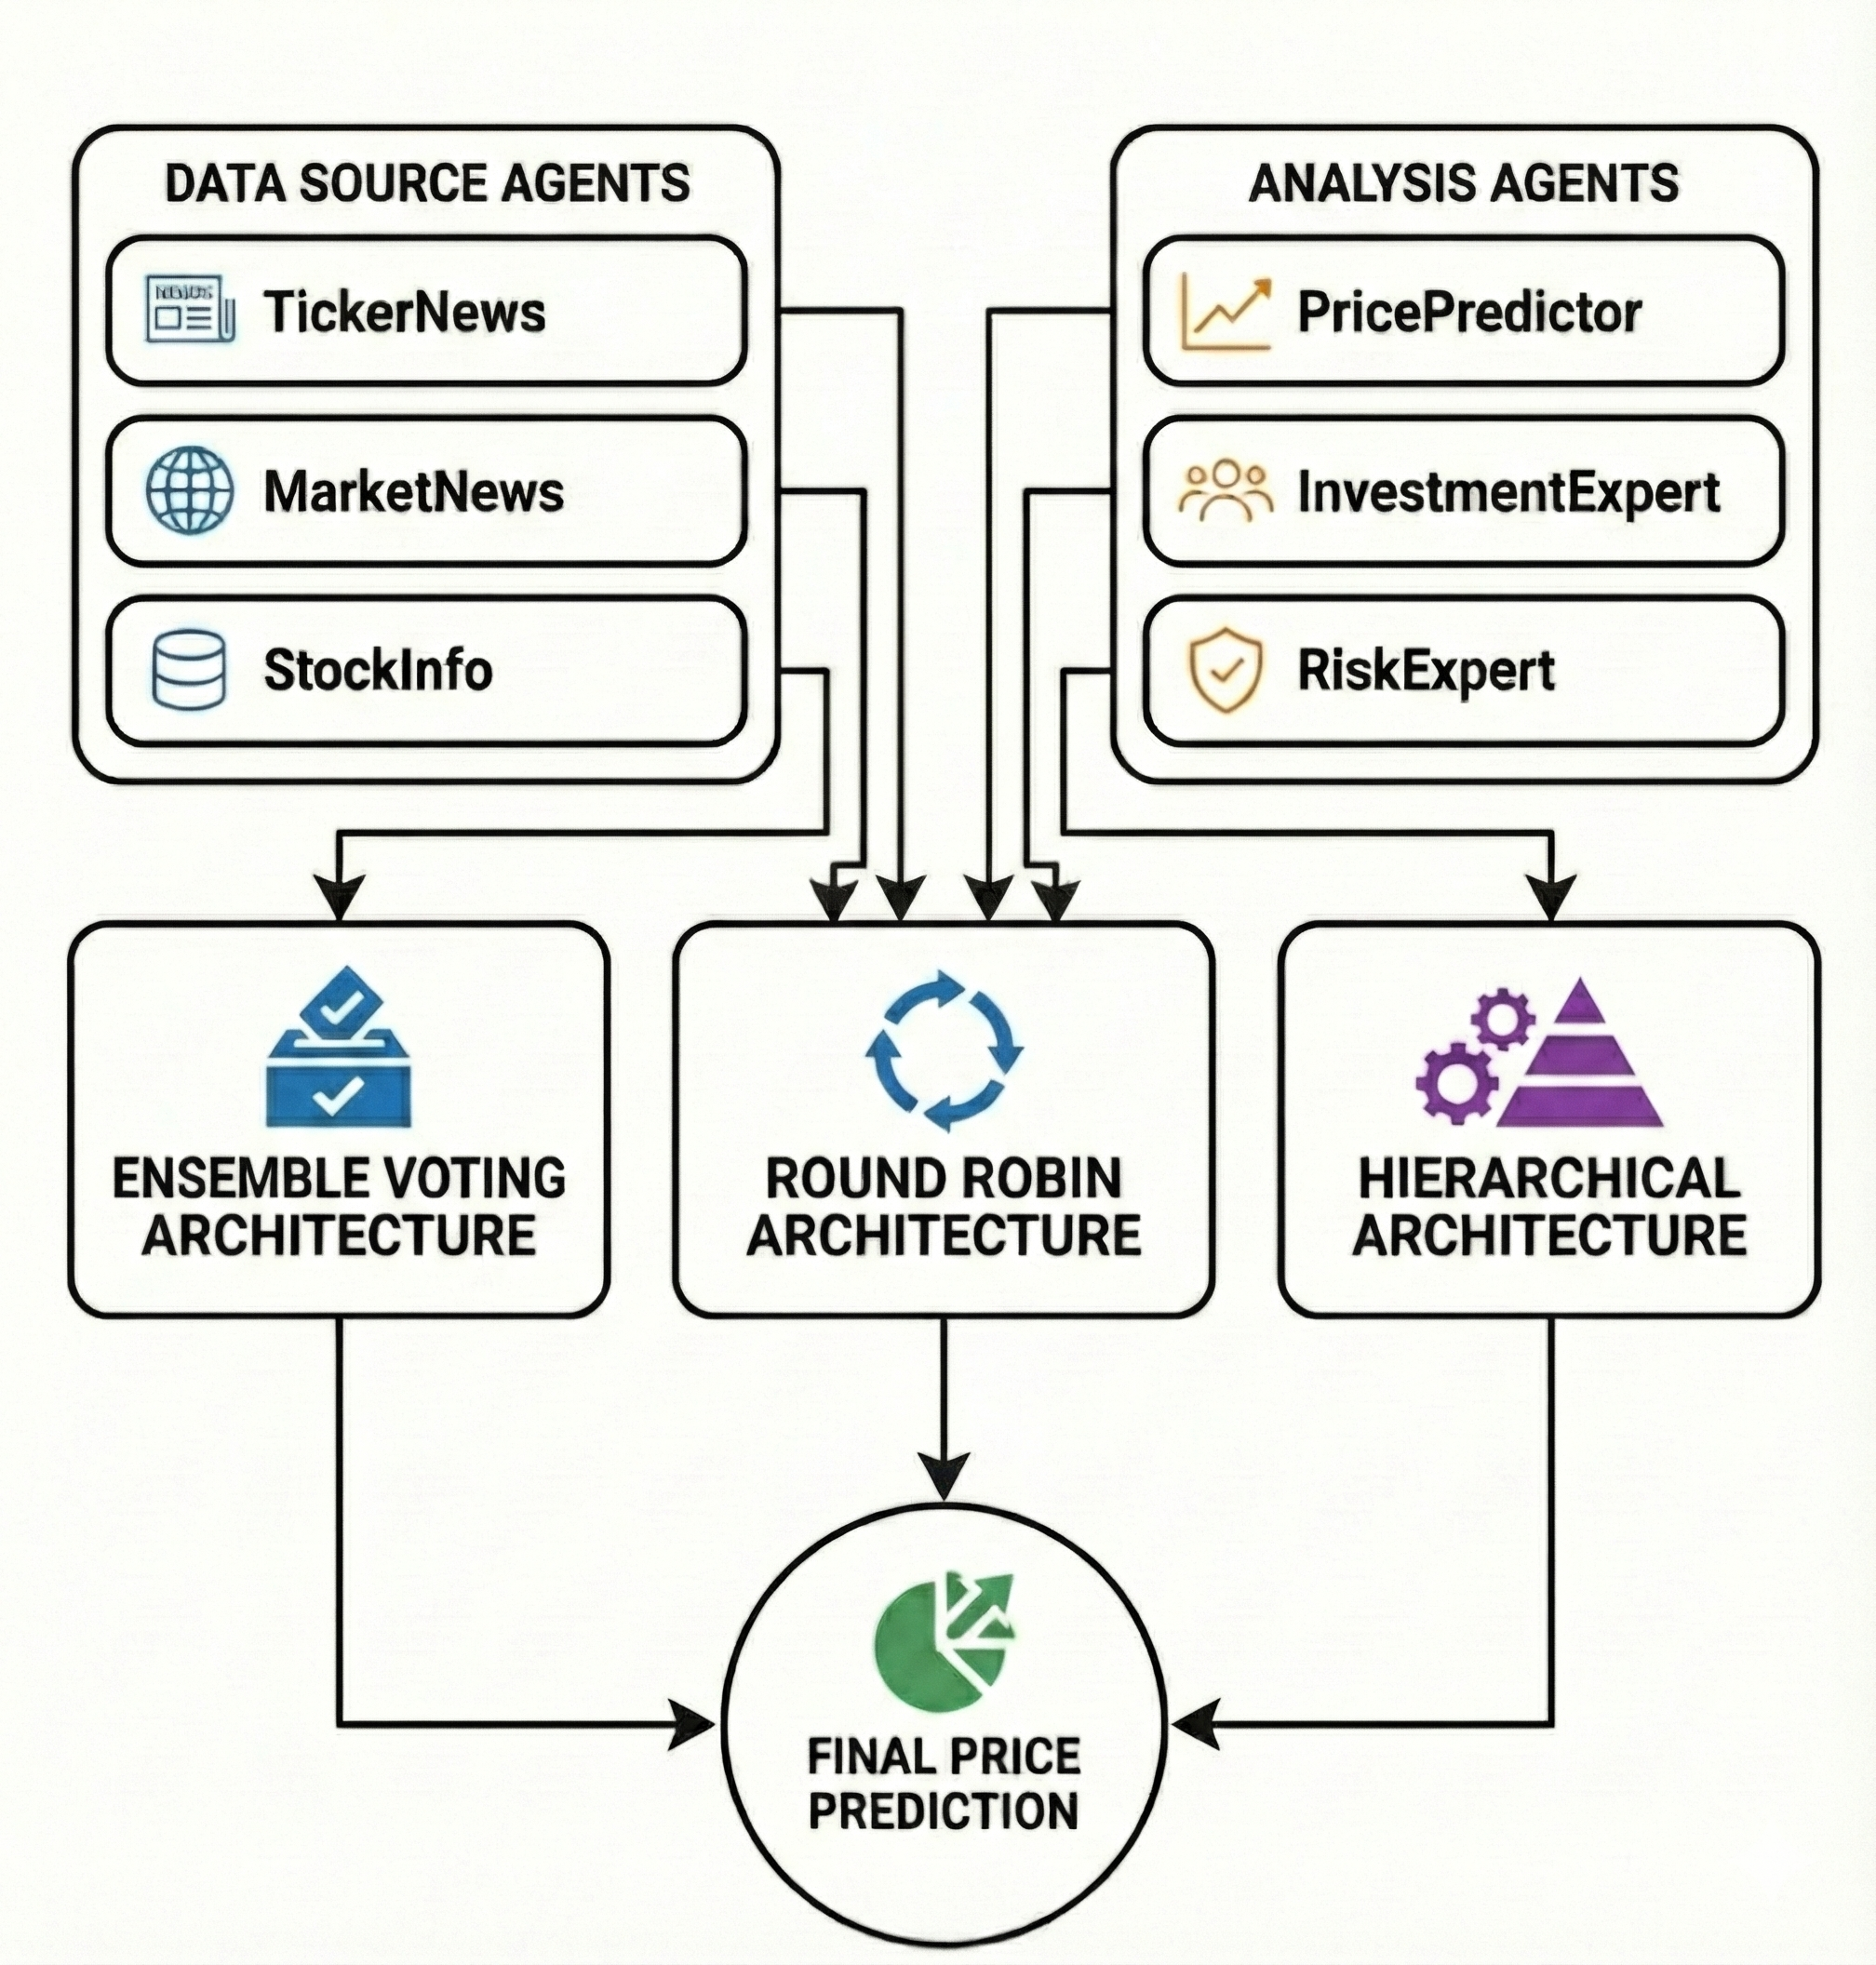
\includegraphics[width=0.9\linewidth]{anh/overallmain.png}
    \caption{
System overview diagram}
    \label{fig:
System overview diagram}
\end{figure}

\subsection{The Specialized Agent Team}
\subsubsection{Agents Overview}
\begin{itemize}
    \item \textbf{PricePredictor Agent:} 
    Uses the primary LSTM forecast blended with technical tools such as the \textbf{Relative Strength Index (RSI)}, \textbf{Moving Average Convergence Divergence (MACD)}, and \textbf{Bollinger Bands}. By analyzing tendencies and momentum, it improves the initial prediction to offer a greater correct rate prediction together with a confidence rating for the technical analysis.

    \item \textbf{InvestmentExpert Agent:} 
    InvestmentExpert Agent: Takes into consideration critical financial numbers which include the \textbf{Price-to-Earnings ratio (P/E)}, \textbf{Price-to-Book ratio (P/B)}, \textbf{Return on Equity (ROE)}, \textbf{Earnings Per Share growth (EPS)}, and \textbf{Debt-to-Equity ratio}. It conducts an intensive assessment of the company`s financial health and growth potential, resulting in a recommendation to \textbf{BUY, SELL, or HOLD}, together with a confidence score for its financial analysis.

    \item \textbf{RiskExpert Agent:} 
    Analyzes volatility profiles, marketplace correlation matrices, and historical drawdown data. It evaluates general portfolio risk via volatility modeling and correlation dynamics, offering a quantified risk stage with corresponding position sizing guidance.

    \item \textbf{TickerNews Agent:} 
    Processes company-specific news sourced from systems including CafeF, VietStock,... and earnings releases. Employing sentiment classification and event-driven effect evaluation, it outputs a sentiment polarity rating coupled with an expected marketplace effect magnitude.

    \item \textbf{MarketNews Agent:} 
    Examines macroeconomic updates, marketplace sentiment data, and valuable bank communications. Through systemic threat evaluation and regime classification, it generates a contextual marketplace rating reflecting prevailing macroeconomic conditions.

    \item \textbf{StockInfo Agent:} 
    Analyzes trading volume, liquidity trends, and technical metadata to assess marketplace microstructure. The agent presents a liquidity-adjusted feasibility score followed through execution-related suggestions for most reliable trade deployment.
\end{itemize}

\subsubsection{LLMs Overview}
In this study, \textbf{Google Gemini 2.0 Flash} is selected as the core LLM due to its high scalability, low-latency cloud execution, and exceptionally large context window, making it well-suited for production-grade AI pipelines. To provide a broader comparative perspective, we additionally include \textbf{OpenAI GPT-4o} and \textbf{Llama-3.1-8b}. GPT-4o is recognized for its strong reasoning quality and balanced multimodal performance, whereas Llama-3.1 offers significant advantages for privacy-focused and offline deployments. The operational characteristics of these models are summarized in Table~\ref{tab:llm_comparison_summary_en}.

\begin{table}[h!]
\centering
\caption{Operational Characteristics and Execution Behavior of Leading Large Language Models.}
\label{tab:llm_comparison_summary_en}
\resizebox{\columnwidth}{!}{
\begin{tabular}{@{}lccc@{}}
\toprule
\textbf{Criterion} & \textbf{Gemini 2.0 Flash} & \textbf{GPT-4o} & \textbf{Llama-3.1-8b} \\ \midrule
Deployment & Cloud API & Cloud API & Local / Hosted \\
Latency & Low & Medium & Low / Variable \\
Throughput & Very High & High & Infra-dependent \\
Offline Capability & None & None & Yes \\
Context Window & Up to 1M tokens & Up to 128k tokens & Model-dependent \\
Cost Model & SaaS (usage-based) & SaaS (usage-based) & CapEx / SaaS \\
Optimized for & Cloud scale & Reasoning quality & Privacy / Control \\ 
\bottomrule
\end{tabular}
}
\end{table}

\subsection{Coordination Architectures}
\subsubsection{Hierarchical Architecture (Design 1)}

\paragraph{Operational Mechanism}
The hierarchical architecture operates under a Master–Subordinate coordination paradigm, in which a single centralized \textit{Master Agent} oversees six \textit{Specialized Agents}, each responsible for processing distinct streams of financial information, including technical indicators, fundamental metrics, portfolio risk profiles, market sentiment, and microstructure data. Each agent functions independently and in parallel, enabling efficient handling of heterogeneous inputs while preserving modular expertise. The \textit{Master Agent} then collects and consolidates all outputs, performing rigorous consistency checks and employing ensemble synthesis techniques to generate a unified, coherent market prediction that reflects multiple analytical perspectives, thereby enhancing reliability, robustness, and interpretability. This design balances computational efficiency with structured integration of diverse financial insights, allowing disparate information sources to interact within a centralized decision-making framework that supports scalable, actionable, and interpretable outcomes. Similar hierarchical coordination principles have been successfully applied in multi-agent financial simulations to improve decision consistency and system scalability~\cite{tesfatsion2006,lebaron2006}.
\\
Furthermore, maintaining modularity at the agent level enables targeted refinement and adaptive learning within individual analytical domains, progressively enhancing predictive accuracy. This multi-layered coordination approach supports robust ensemble predictions while providing a transparent framework to trace each analytical stream’s contribution to the final market decision, thereby reinforcing interpretability and trustworthiness in complex financial environments.

\begin{figure}[H]
    \centering
    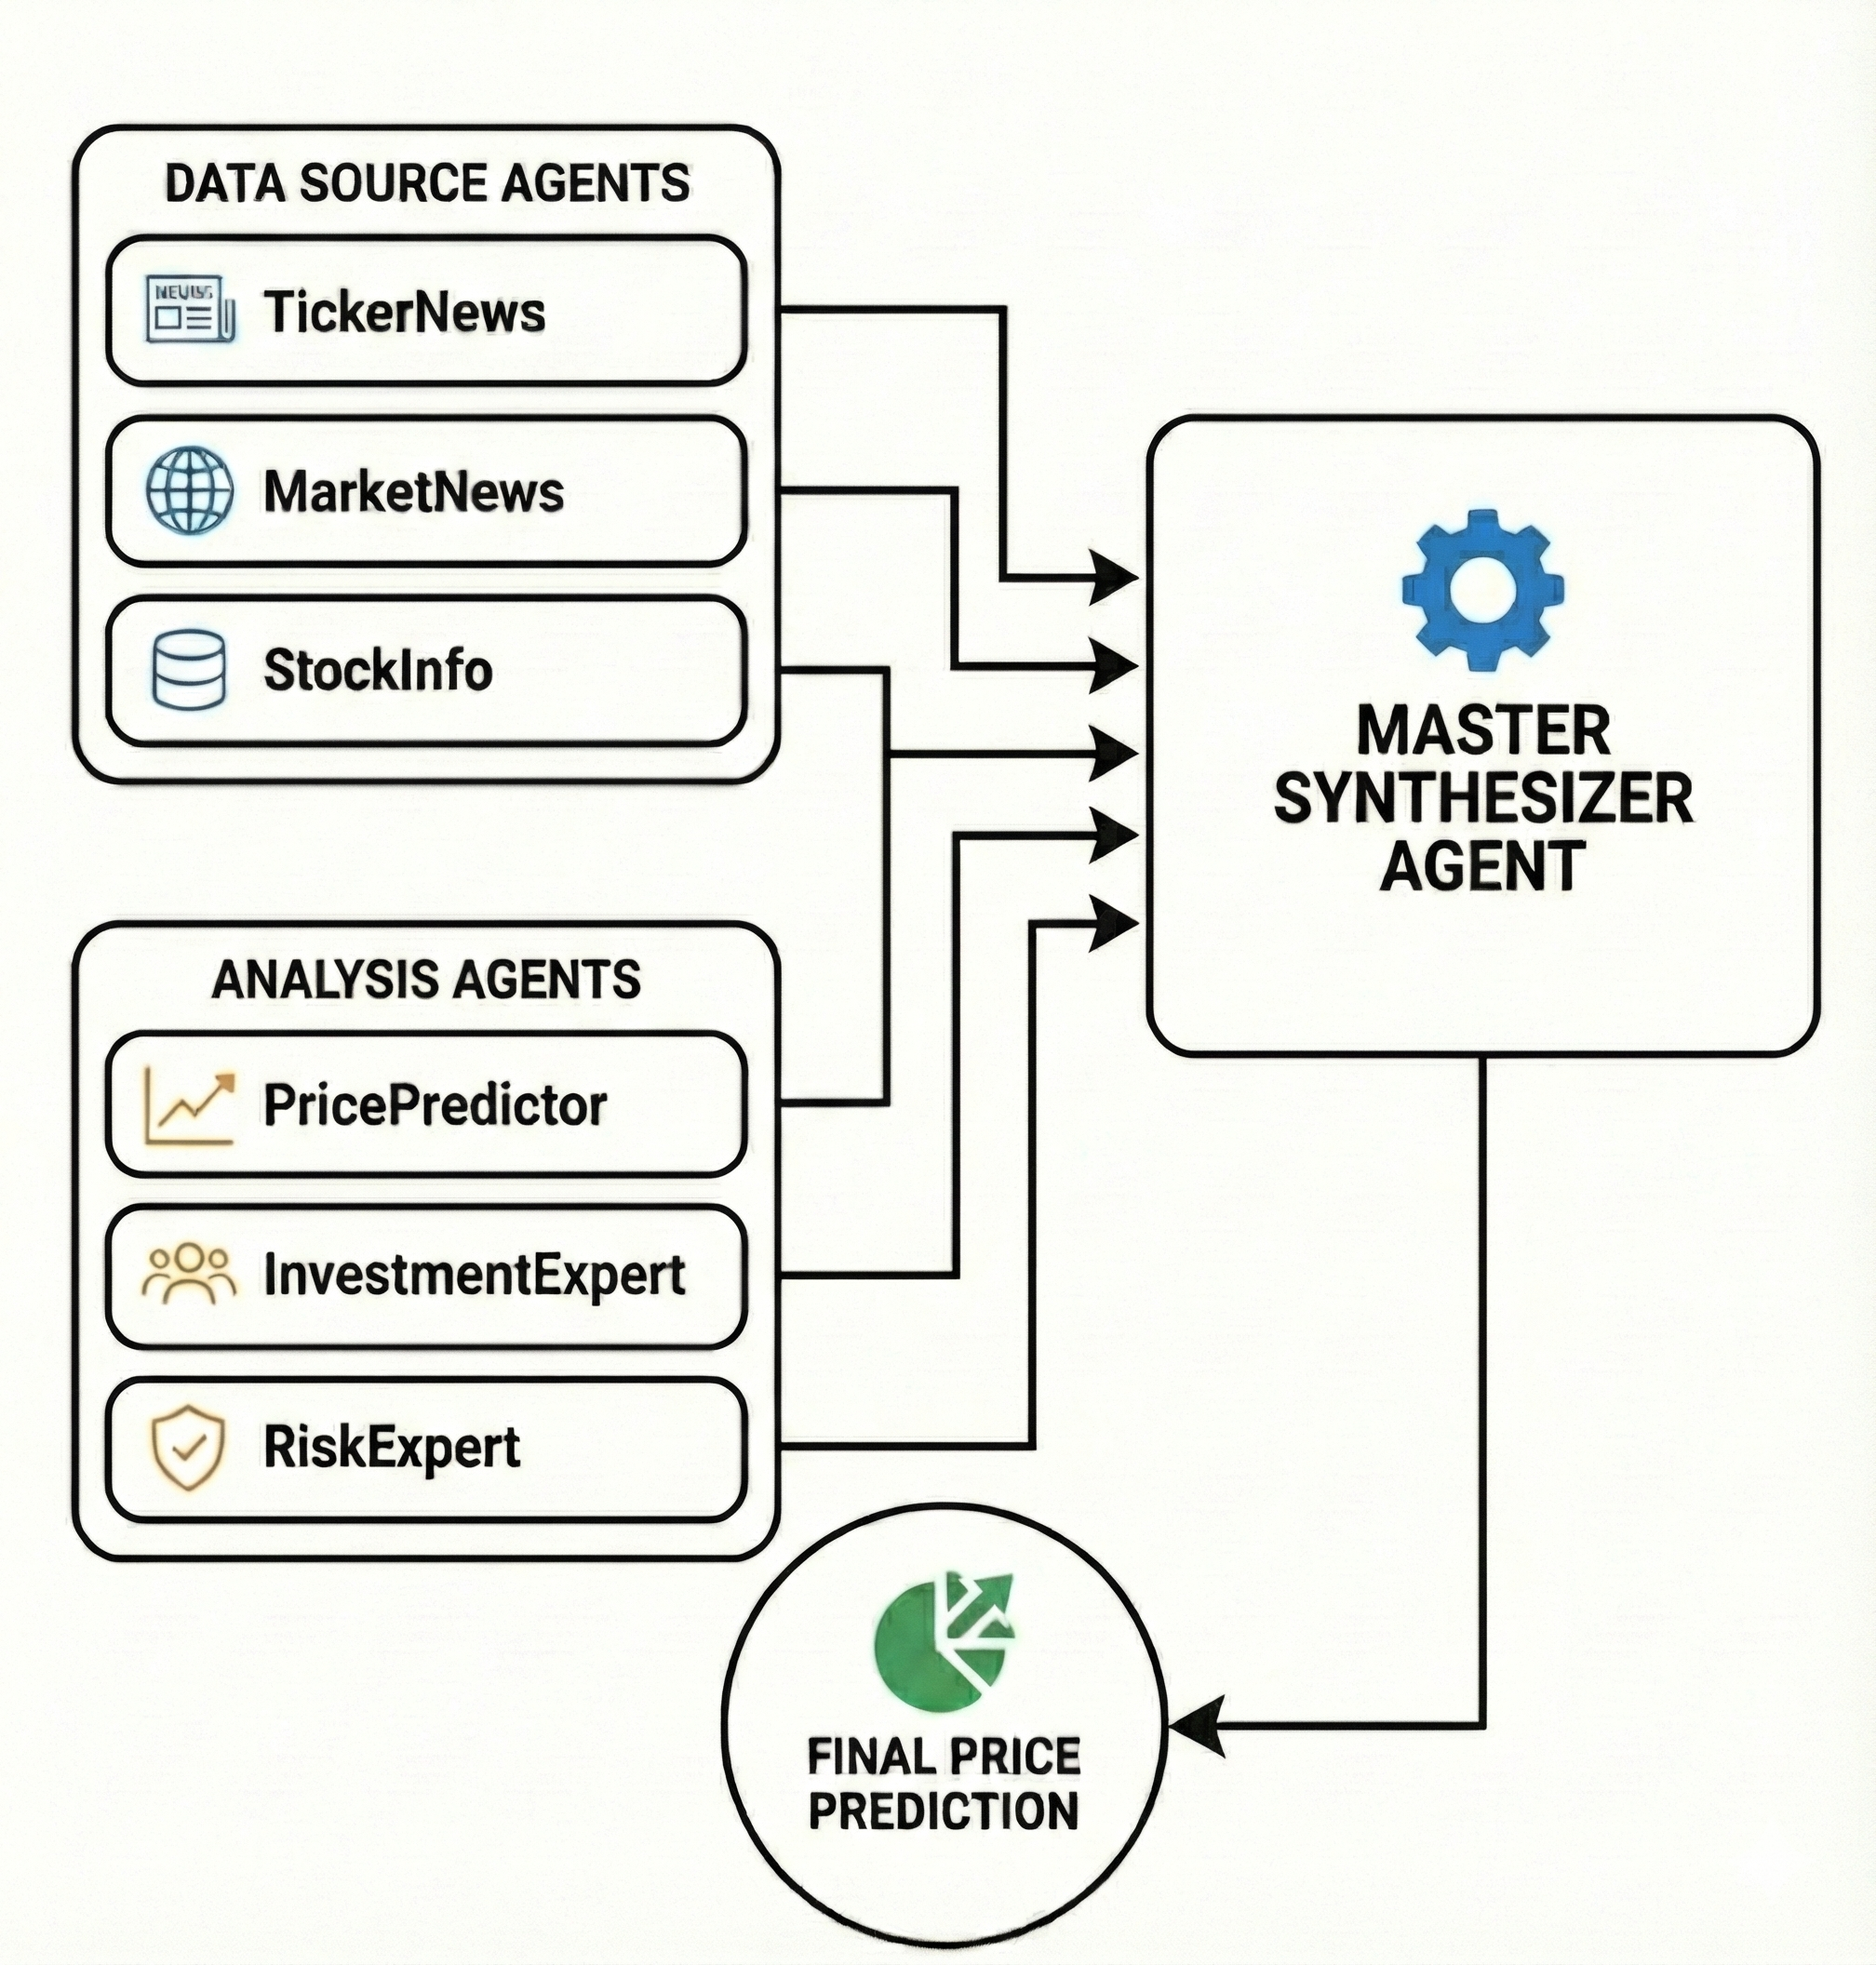
\includegraphics[width=0.9\linewidth]{anh/hiemain.png}
    \caption{Hierarchical architecture with a Master Agent coordinating six specialized agents. Each agent processes domain-specific data in parallel, and the Master Agent aggregates outputs for final prediction.}
    \label{fig:hierarchical_architecture}
\end{figure}


\paragraph{Workflow}
The hierarchical architecture operates through a structured sequence of five key stages:

\begin{enumerate}
    \item \textbf{Data Acquisition and Preprocessing} — 
    The system collects and preprocesses multi-source financial data, including technical indicators, fundamental ratios, and market sentiment signals.
    
    \item \textbf{LSTM Foundation Modeling} — 
    An LSTM-based model generates the initial price prediction, serving as the base signal for subsequent multi-agent analysis.
    
    \item \textbf{Parallel Agent Processing} — 
    Six specialized agents operate simultaneously, each focusing on a distinct analytical dimension such as risk assessment, fundamental valuation, and news sentiment interpretation.
    
    \item \textbf{Master Agent Aggregation} — 
    The Master Agent consolidates all intermediate outputs, performing validation and consistency checks to ensure model reliability and coherence.
    
    \item \textbf{Final Output Generation} — 
    The system produces the unified result, including final price forecasts, confidence levels, and investment recommendations.
\end{enumerate}

\subsubsection{Round Robin Architecture (Design 2)}
\paragraph{Operational Mechanism}
The Round Robin architecture follows a sequential refinement process, in which every agent receives the output from the former stage, improves it by the use of its specialized analysis, and passes it forward. This iterative chain allows modern development of predictions via multi-perspective evaluation \cite{wang2021,tesfatsion2006,lebaron2006,chen2012}. 


\begin{figure}[H]
    \centering
    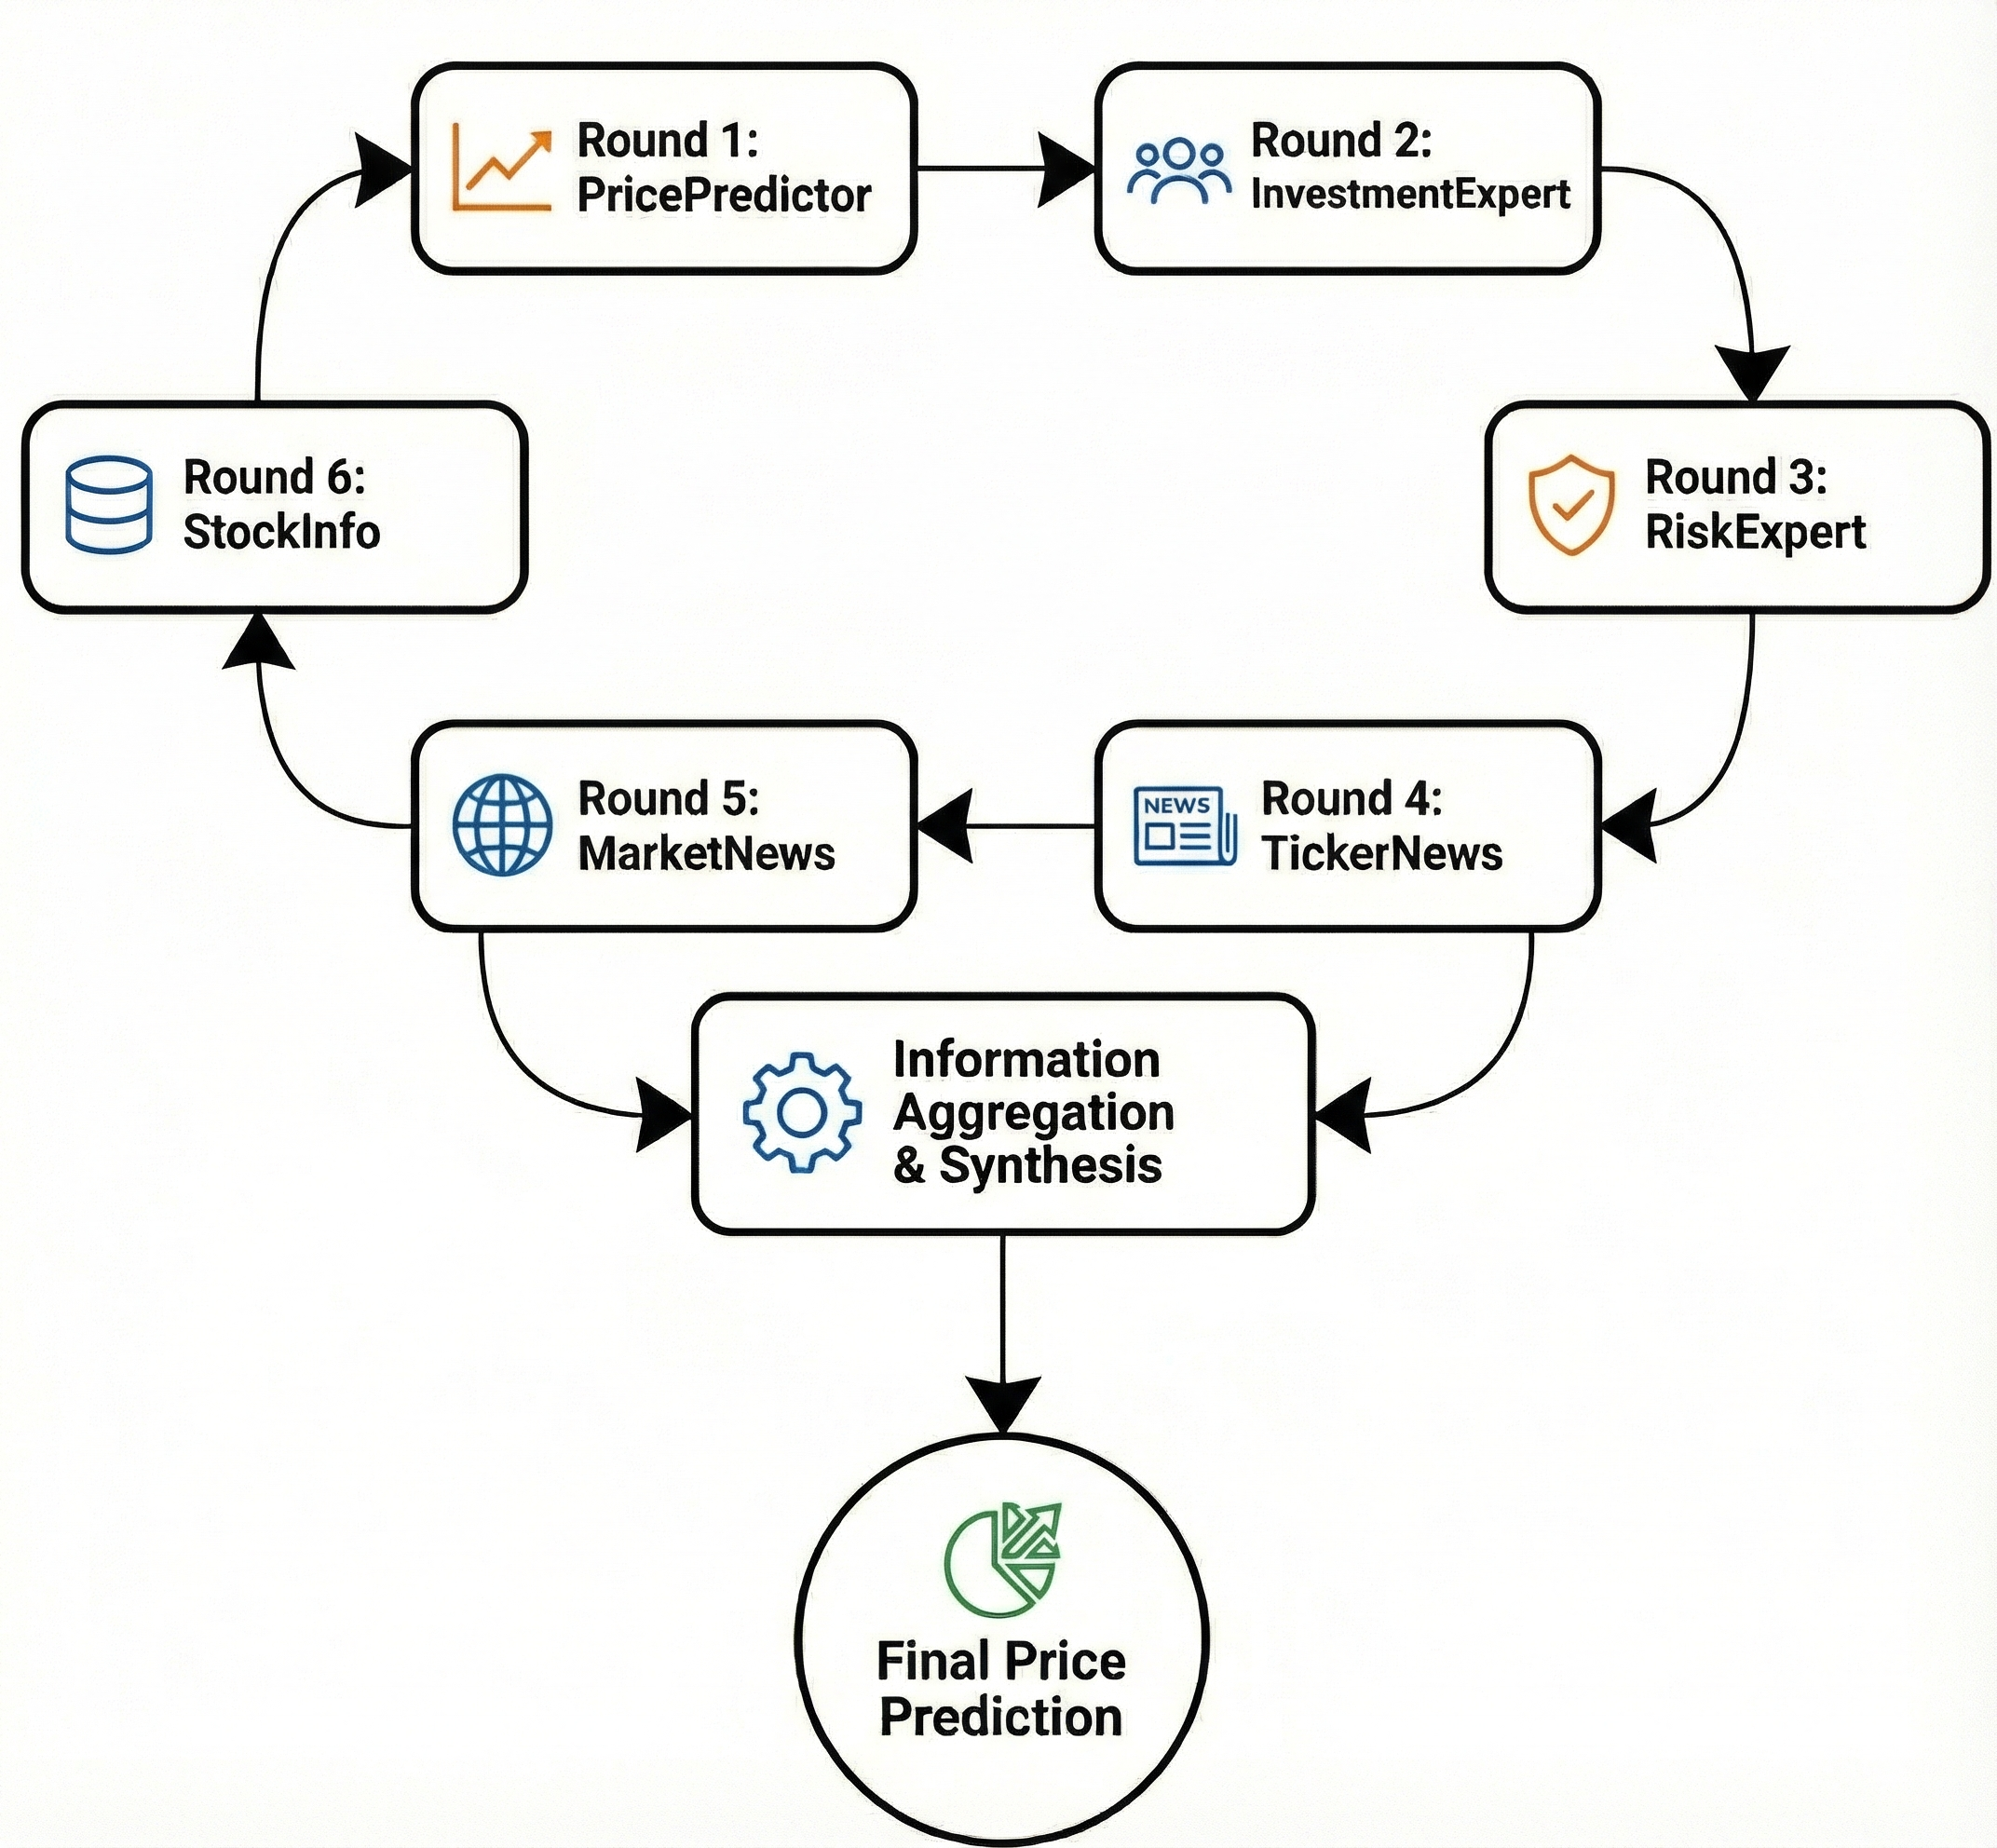
\includegraphics[width=0.9\linewidth]{anh/rrmain.png}
    \caption{Round Robin architecture with six specialized agents operating in a sequential refinement cycle.}
    \label{fig:hierarchical_architecture}
\end{figure}



\paragraph{Workflow} The round robin operates via an organized sequence of distinct stages:

\begin{enumerate}
    \item \textbf{Initialization.} The approach begins with the  \textit{LSTM Foundation Layer}, which constructs the initial predictive state by capturing temporal dependencies in the historical data. This state serves as the baseline representation of the market dynamics before any domain-specific refinement is applied.  

    \item \textbf{Sequential Agent Flow.} The predictive state is propagated through six specialized agents in a fixed order: Round~1 $\rightarrow$ Round~2 $\rightarrow$ Round~3 $\rightarrow$ Round~4 $\rightarrow$ Round~5 $\rightarrow$ Round~6. Each agent operates as a refinement node, sequentially receiving the previous output, performing its own analysis, and forwarding an improved result to the subsequent stage.  

    \item \textbf{Incremental Enhancement.} Within this Round Robin structure, every agent contributes a unique perspective—technical, fundamental, risk-based, news-driven, or macroeconomic—to enrich the evolving state. This iterative enhancement ensures that both micro-level indicators and macro-level contexts are systematically embedded into the prediction pipeline.  

    \item \textbf{Decision Traceability.} Throughout the refinement sequence, all intermediate states and analytical decisions are logged to preserve a transparent audit trail. This traceability allows researchers and practitioners to examine how individual agents influenced the outcome, thereby supporting interpretability and trust in model-driven recommendations.  

    \item \textbf{Cumulative Refinement Output.} Upon completion of the six-round iteration, the framework consolidates the results into a final state representing the cumulative learning and multi-perspective reasoning of the entire agent ensemble. The resulting output thus reflects not only predictive accuracy but also contextual awareness and adaptive decision integration across the full refinement cycle.  
\end{enumerate}

\subsubsection{Ensemble Voting Architecture (Design 3)}
\paragraph{Operational Mechanism}
The Ensemble Voting Architecture employs an intelligent voting system in which six specialized agents operate concurrently and independently. Every agent carries out focused studies on different data fields, which ensures that a wide range of predictive angles are taken into account. After this, the system uses a statistical inference engine to combine these findings. This engine makes use of dynamic weighting according to the recent performance, execution time, and confidence score. This versatile strategy improves robustness and reduces bias, facilitating more dependable and easily understood collective predictions within financial predictions~\cite{opera2023}.

\begin{figure}[H]
    \centering
    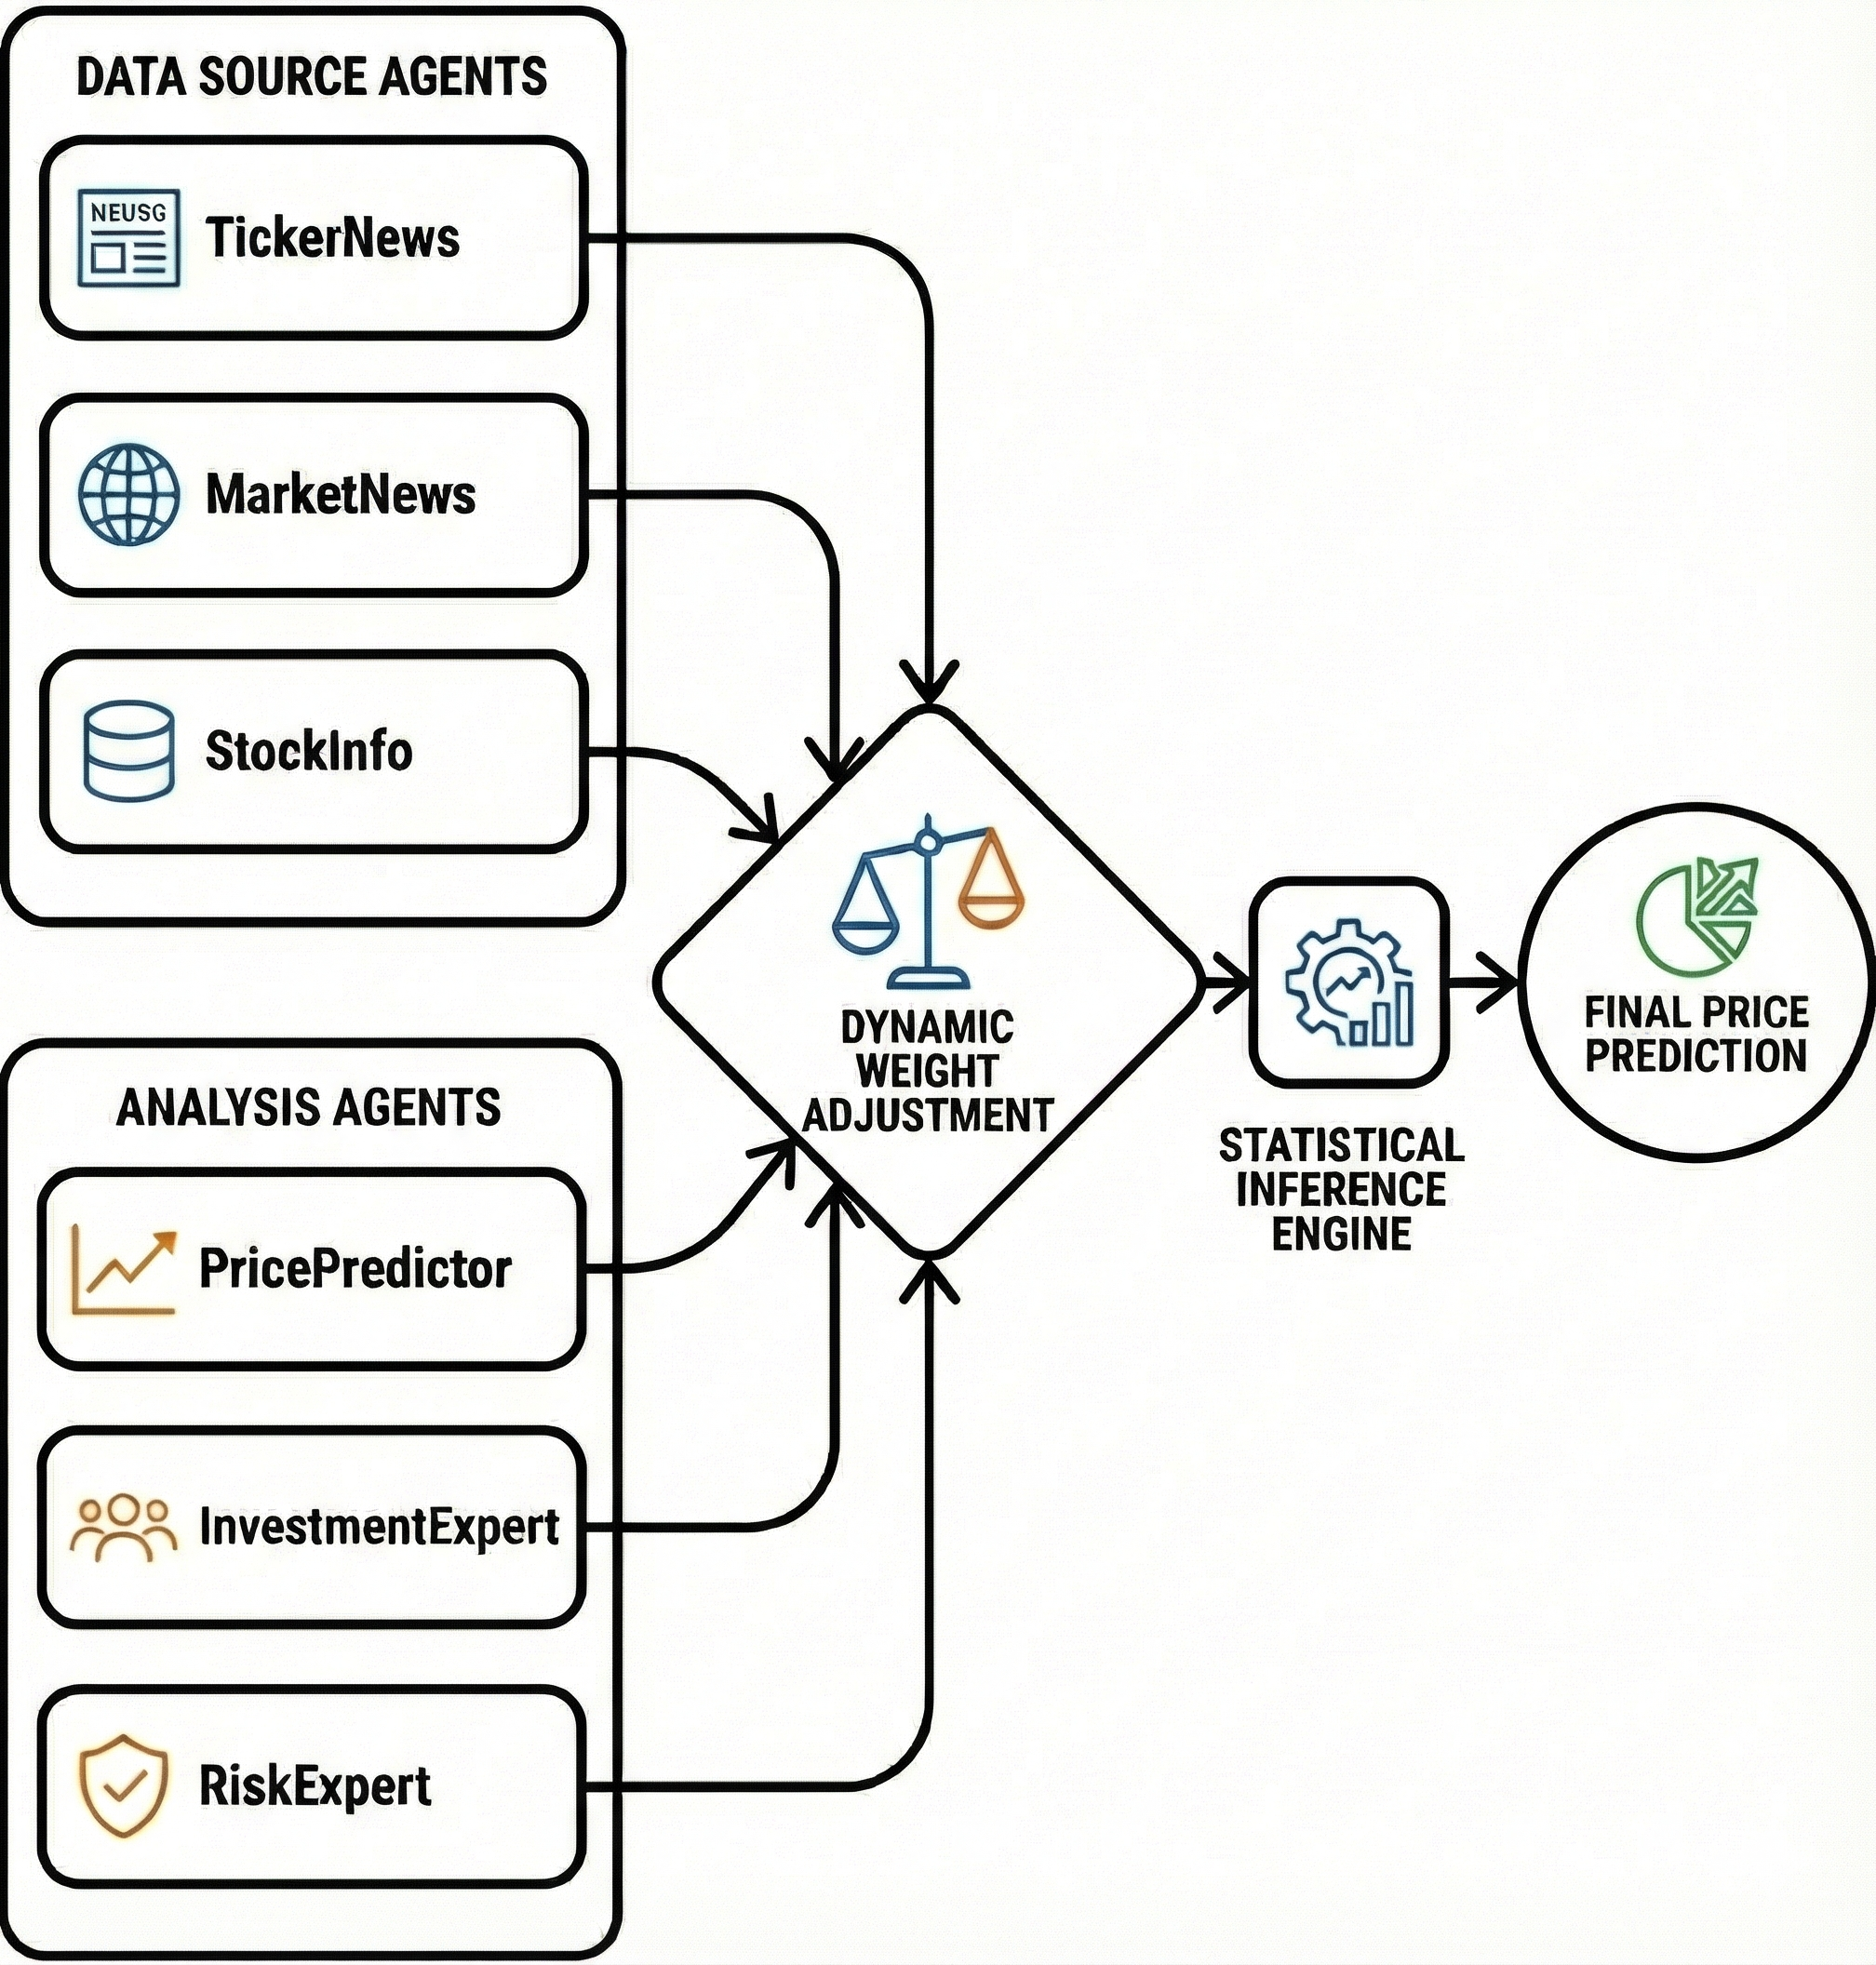
\includegraphics[width=0.9\linewidth,height=8cm]{anh/emmain.png}
    \caption{Ensemble Voting Architecture  with six specialized agents employing an intelligent voting }
    \label{fig:hierarchical_architecture}
\end{figure}


\paragraph{Workflow}
The operational flow of the proposed Ensemble Voting Architecture is summarized as follows:

\begin{enumerate}
    \item \textbf{Data Distribution:} Input data streams are concurrently distributed to all six agents.
    \item \textbf{Parallel Processing:} Each agent operates independently in parallel, ensuring full task isolation.
    \item \textbf{Performance Evaluation:} Real-time assessment of individual agent performance is continuously conducted.
    \item \textbf{Dynamic Weight Adjustment:} Model weights are adaptively updated based on the latest performance metrics.
    \item \textbf{Statistical Inference Integration:} Final aggregation is performed through statistical inference with uncertainty quantification to enhance predictive reliability.
\end{enumerate}




\paragraph{Dynamic Weight Adjustment Process}
To maintain adaptiveness in a volatile environment, the model employs a continuous weight adjustment mechanism.  
First, each agent’s recent performance is evaluated through multiple metrics including prediction accuracy, confidence calibration, and execution latency.  
Second, agent weights are updated proportionally to recent efficiency, ensuring that higher-performing agents exert greater influence.  
Third, normalization is applied to maintain a total ensemble weight of unity.  
Lastly, real-time optimization enables the system to react dynamically to shifting market conditions, preserving robustness and responsiveness over time.\cite{McAndrew2021,Lu2023}

\paragraph{Statistical Inference Process}
The ensemble layer integrates all agent outputs through a statistically grounded inference procedure.  
Predictions are first aggregated using dynamically adjusted weights to produce a composite forecast.  
Uncertainty quantification is then conducted via variance estimation to assess reliability.  
Consensus analysis measures inter-agent agreement, capturing alignment across diverse analytical dimensions.  
Finally, statistical validation is performed to verify the ensemble’s internal coherence and predictive soundness, ensuring that aggregated outputs remain both consistent and interpretable in empirical contexts (see e.g., \cite{wang2021,li2022}). 






\section{Empirical Evaluation}
\subsection{Research Questions (RQs)}
To rigorously assess the effectiveness of our proposed framework, \textsc{Multi-Agent Vietnam Stock}, we design our empirical study around the following research questions:

\textbf{RQ1. [Coordination Effectiveness]}  
Which coordination architecture (Hierarchical, Round Robin, or Ensemble) is the most effective for the Vietnamese stock market?

\textbf{RQ2. [Multi-Agent vs. Single-Agent Architectures vs Machine Learning Baseline]}  
Does the Multi-Agent system outperform traditional Single-Agent (Gemini) and LSTM models?


\subsection{Dataset \& Settings}
A fundamental structural characteristic of the Vietnamese stock market is its \textbf{T+2.5 settlement period}. Given that \textit{domestic individual investors overwhelmingly dominate the market, accounting for approximately 85-90\% of daily trading value} \cite{TinNhanhChungkhoan2025}, this configuration strongly incentivizes rapid, short-term speculative trading. This retail-heavy structure, often characterized by significant \textit{herd behavior} rather than fundamental analysis, is identified by analysts as a primary driver of the market's notoriously high price volatility \cite{WorldBank2024, Yuanta2025}.



Inspired by the substantial effects of this behavioral pattern, the present study conducts a sector-specific analysis by selecting representative stocks from four key sectors of the Vietnamese economy: \textbf{Banking (VCB)}, \textbf{Technology (FPT)}, \textbf{Real Estate (DXG)}, and \textbf{Industrial Construction (VCS)}. These sectors are chosen to capture the structural diversity of the Vietnamese stock market in terms of regulation intensity, growth potential, and sensitivity to macroeconomic conditions.

VCB represents the banking sector due to its large market capitalization, high liquidity, and systemic importance within Vietnam’s financial system, making it highly sensitive to monetary policy and regulatory changes. FPT is selected as a proxy for the technology sector, where price movements are largely driven by innovation, earnings growth, and investor sentiment. DXG reflects the real estate sector, which is characterized by strong cyclicality and elevated volatility arising from credit conditions and macroeconomic fluctuations. Finally, VCS represents the industrial construction sector, whose stock performance is closely linked to infrastructure investment, export demand, and long-term development cycles, typically exhibiting more stable yet trend-driven behavior.

This diversified sectoral selection enables a comprehensive evaluation of forecasting performance across heterogeneous market dynamics.


To rigorously evaluate predictive performance across heterogeneous investment horizons, the 
analysis is structured into three temporal regimes:
\begin{itemize}
    \item \textbf{Short-term (3 days):} aligned with the T+2.5 settlement window, capturing immediate speculative turnover.
    \item \textbf{Medium-term (14 days):} representing a conventional tactical positioning horizon.
    \item \textbf{Long-term (60 days):} proxying strategic buy-and-hold investment behavior.
\end{itemize}

To ensure robustness and reduce temporal bias, the evaluation at each forecasting horizon (\textbf{Short-term}, \textbf{Medium-term}, \textbf{Long-term}) is conducted across four distinct market intervals:
\begin{enumerate}
    \item \textbf{Late August to early September}: capturing post-summer liquidity shifts;
    \item \textbf{16/10/2025}: representing a period of heightened trading activity;
    \item \textbf{21/10/2025}: corresponding to a stabilization phase after short-term volatility;
    \item \textbf{22/10/2025}: reflecting market behavior during an immediate rebound window.
\end{enumerate}
Assessing performance across these four checkpoints enables a comprehensive examination of model behavior under varying liquidity, volatility, and sentiment conditions, thereby strengthening the validity of comparative results across all three time horizons.


\subsection{Evaluation Metrics.} 
To rigorously evaluate the predictive performance of the proposed framework, this study utilizes three established statistical indicators: Mean Absolute Error (MAE), Root Mean Square Error (RMSE), and Mean Absolute Percentage Error (MAPE). MAE quantifies the average magnitude of errors in a set of forecasts without considering their direction, providing a linear score that weights all individual differences equally~\cite{willmott2005advantages}. Conversely, RMSE operates as a quadratic scoring rule; by squaring residuals prior to averaging, it assigns greater weight to larger deviations, thereby increasing sensitivity to outliers~\cite{chai2014root}. Finally, MAPE measures accuracy as a relative percentage, facilitating the comparison of forecasting performance across datasets with differing scales~\cite{hyndman2006another}.

\section{Coordination Effectiveness (RQ1)}
This section addresses the first research question by comparing the coordination effectiveness of three multi-agent architectures: \textit{Hierarchical}, \textit{Round Robin}, and \textit{Ensemble Voting}. Coordination effectiveness is defined as the ability to manage interactions among forecasting agents to produce stable and accurate predictions under varying market conditions. This evaluation is particularly relevant in the Vietnamese stock market, which is characterized by high volatility and frequent regime shifts.

To assess adaptability and robustness, we evaluate predictive performance across short-term, medium-term, and long-term forecasting horizons, capturing both rapid market fluctuations and longer-term trends. The Hierarchical architecture employs centralized aggregation to enhance stability, potentially at the cost of responsiveness. Round Robin enables sequential refinement and adaptability but may be vulnerable to error propagation. Ensemble Voting aggregates parallel predictions, aiming to reduce individual model bias through collective decision-making.

Our analysis considers predictive accuracy, directional consistency, and error variability across stocks and horizons to evaluate robustness. The results provide insights into how different coordination strategies balance stability and flexibility in volatile emerging markets, forming the basis for subsequent architectural comparisons and deployment considerations.


\subsection{Qualitative Results}

\clearpage
\onecolumn

\begin{table*}[!h]
\centering
\caption{Comparison of Short-term, Medium-term, and Long-term Forecasts Across Architectures and Stocks (LLM: Google Gemini 2.0 Flash)}
\label{tab:full_forecast}
\setlength{\tabcolsep}{3pt}
\renewcommand{\arraystretch}{1.05}
\scriptsize
\begin{tabular}{llcc|cccc|cccc|cccc}
\toprule
\multirow{2}{*}{\textbf{Stock}} &
\multirow{2}{*}{\textbf{Architecture}} &
\multicolumn{2}{c|}{\textbf{Start}} &
\multicolumn{4}{c|}{\textbf{Short-term}} &
\multicolumn{4}{c|}{\textbf{Medium-term}} &
\multicolumn{4}{c}{\textbf{Long-term}} \\
\cmidrule(lr){3-4}
\cmidrule(lr){5-8}
\cmidrule(lr){9-12}
\cmidrule(lr){13-16}
& &
\textbf{Date} & \textbf{Price} &
\textbf{End Date} & \textbf{Pred} & \textbf{Act} & \textbf{Gap} &
\textbf{End Date} & \textbf{Pred} & \textbf{Act} & \textbf{Gap} &
\textbf{End Date} & \textbf{Pred} & \textbf{Act} & \textbf{Gap} \\
\midrule


%%%%%%%%%%%%%%%%%%%%%%%%%%%%%%%%%%%%%%%%%%%%%%%%%%%%%%%%%%%%%%%%%%%%%%%%%%%%%%%%%%%%
% ===================== DXG ======================
%%%%%%%%%%%%%%%%%%%%%%%%%%%%%%%%%%%%%%%%%%%%%%%%%%%%%%%%%%%%%%%%%%%%%%%%%%%%%%%%%%%%
\multirow{4}{*}{\textbf{DXG}} 
& \textbf{Hierarchical}
& 31/08 & 22.8 & 03/09 & 22.25 & 24 & 0.63 & 14/09 & 23.38 & 24.05 & 0.63 & 30/10 & 21.83 & 21.2 & 0.63 \\

& 
& 16/10 & 22.45 & 19/10 & 22.10 & 22.6 & 8.16 & 30/10 & 23.34 & 21.2 & 8.16 & 15/12 & 24.46 & 16.3 & 8.16 \\

& 
& 21/10 & 20.0 & 24/10 & 20.51 & 20.9 & 3.01 & 04/11 & 20.52 & 20.15 & 3.01 & 20/12 & 20.81 & 17.8 & 3.01 \\

&
& 22/10 & 20.5 & 25/10 & 21.10 & 20.9 & 2.62 & 05/11 & 28.88 & 20.1 & 2.62 & 21/12 & 20.42 & 17.8 & 2.62 \\
\midrule


\multirow{4}{*}{\textbf{DXG}} 
& \textbf{Round Robin}
& 31/08 & 22.8 & 03/09 & 22.25 & 24 & 3.27 & 14/09 & 21.98 & 24.05 & 3.27 & 30/10 & 24.47 & 21.2 & 3.27 \\

&
& 16/10 & 22.45 & 19/10 & 22.15 & 22.6 & 9.33 & 30/10 & 22.28 & 21.2 & 9.33 & 15/12 & 25.63 & 16.3 & 9.33 \\

&
& 21/10 & 20.0 & 24/10 & 20.34 & 20.9 & 3.16 & 04/11 & 20.79 & 20.15 & 3.16 & 20/12 & 20.96 & 17.8 & 3.16 \\

&
& 22/10 & 20.5 & 25/10 & 20.48 & 20.9 & 3.16 & 05/11 & 23.68 & 20.1 & 3.16 & 21/12 & 20.96 & 17.8 & 3.16 \\
\midrule


\multirow{4}{*}{\textbf{DXG}} 
& \textbf{Ensemble}
& 31/08 & 22.8 & 03/09 & 22.11 & 24 & 0.27 & 14/09 & 22.98 & 24.05 & 0.27 & 30/10 & 21.47 & 21.2 & 0.27 \\

&
& 16/10 & 22.45 & 19/10 & 21.92 & 22.6 & 7.06 & 30/10 & 21.75 & 21.2 & 7.06 & 15/12 & 23.36 & 16.3 & 7.06 \\

&
& 21/10 & 20.0 & 24/10 & 20.07 & 20.9 & 3.01 & 04/11 & 20.52 & 20.15 & 3.01 & 20/12 & 20.81 & 17.8 & 3.01 \\

&
& 22/10 & 20.5 & 25/10 & 21.05 & 20.9 & 2.65 & 05/11 & 26.35 & 20.1 & 2.65 & 21/12 & 20.45 & 17.8 & 2.65 \\
\midrule



%%%%%%%%%%%%%%%%%%%%%%%%%%%%%%%%%%%%%%%%%%%%%%%%%%%%%%%%%%%%%%%%%%%%%%%%%%%%%%%%%%%%
% ===================== FPT ======================
%%%%%%%%%%%%%%%%%%%%%%%%%%%%%%%%%%%%%%%%%%%%%%%%%%%%%%%%%%%%%%%%%%%%%%%%%%%%%%%%%%%%
\multirow{4}{*}{\textbf{FPT}} 
& \textbf{Hierarchical}
& 01/09 & 101.6 & 04/09 & 103.60 & 105 & 1.67 & 15/09 & 106.07 & 101.9 & 1.67 & 31/10 & 105.57 & 103.9 & 1.67 \\

&
& 16/10 & 89.8 & 19/10 & 90.83 & 88.1 & 1.67 & 30/10 & 89.32 & 102.7 & 1.67 & 15/12 & 92.13 & 93.8 & 1.67 \\

&
& 21/10 & 93 & 24/10 & 95.37 & 97.7 & 3.66 & 04/11 & 95.80 & 103.3 & 3.66 & 20/12 & 97.56 & 93.9 &3.66\\

&
& 22/10 & 97 & 25/10 & 93.5 & 97.7 & 15.02 & 05/11 & 97.60 & 100.9 & 15.02 & 21/12 & 108.92 & 93.9 & 15.02 \\
\midrule


\multirow{4}{*}{\textbf{FPT}} 
& \textbf{Round Robin}
& 01/09 & 101.6 & 04/09 & 104.42 & 105 & 0.37 & 15/09 & 105.66 & 101.9 & 0.37 & 31/10 & 104.27 & 103.9 & 0.37 \\

&
& 16/10 & 89.8 & 19/10 & 90.46 & 88.1 & 3.10 & 30/10 & 91.28 & 102.7 & 3.10 & 15/12 & 90.70 & 93.8 & 3.10 \\

&
& 21/10 & 93 & 24/10 & 96.00 & 97.7 & 3.58 & 04/11 & 95.25 & 103.3 & 3.58 & 20/12 & 97.48 & 93.9 & 3.58 \\

&
& 22/10 & 97 & 25/10 & 93.68 & 97.7 & 15.02 & 05/11 & 93.60 & 100.9 & 15.02 & 21/12 & 108.92 & 93.9 & 15.02 \\
\midrule



\multirow{4}{*}{\textbf{FPT}} 
& \textbf{Ensemble}
& 01/09 & 101.6 & 04/09 & 103.60 & 105 & 1.13 & 15/09 & 103.6 & 101.9 & 1.13 & 31/10 & 102.77 & 103.9 & 1.13 \\

&
& 16/10 & 89.8 & 19/10 & 88.55 & 88.1 & 1.56 & 30/10 & 91.17 & 102.7 & 1.56 & 15/12 & 92.24 & 93.8 & 1.56 \\

&
& 21/10 & 93 & 24/10 & 95.14 & 97.7 & 3.32 & 04/11 & 96.26 & 103.3 & 3.32 & 20/12 & 97.22 & 93.9 & 3.32 \\

&
& 22/10 & 97 & 25/10 & 96.59 & 97.7 & 11.43 & 05/11 & 97.93 & 100.9 & 11.43 & 21/11 & 105.33 & 93.9 & 11.43 \\
\midrule




%%%%%%%%%%%%%%%%%%%%%%%%%%%%%%%%%%%%%%%%%%%%%%%%%%%%%%%%%%%%%%%%%%%%%%%%%%%%%%%%%%%%
% ===================== VCB ======================
%%%%%%%%%%%%%%%%%%%%%%%%%%%%%%%%%%%%%%%%%%%%%%%%%%%%%%%%%%%%%%%%%%%%%%%%%%%%%%%%%%%%
\multirow{4}{*}{\textbf{VCB}} 
& \textbf{Hierarchical}
& 30/08 & 68.6 & 02/09 & 68.66 & 68.6 & 6.90 & 13/09 & 68.52 & 65.8 & 6.90 & 29/10 & 67.6 & 60.7 & 6.90 \\

&
& 16/10 & 62.9 & 19/10 & 63.29 & 61.9 & 7.67 & 30/10 & 64.29 & 60.6 & 7.67 & 15/12 & 64.47 & 56.8 & 7.67 \\

&
& 21/10 & 59.3 & 24/10 & 61.68 & 59.5 & 1.00 & 04/11 & 62.37 & 60.1 & 1.00 & 20/12 & 58.5 & 57.5 & 1.00 \\

&
& 22/10 & 59.6 & 25/10 & 61.21 & 59.5 & 5.26 & 05/11 & 62.37 & 60.8 & 5.26 & 21/12 & 62.76 & 57.5 & 5.26 \\
\midrule


\multirow{4}{*}{\textbf{VCB}} 
& \textbf{Round Robin}
& 30/08 & 68.6 & 02/09 & 68.46 & 68.6 & 17.11 & 13/09 & 68.9 & 65.8 & 17.11 & 29/10 & 77.81 & 60.7 & 17.11 \\

&
& 16/10 & 62.9 & 19/10 & 62.51 & 61.9 & 7.77 & 30/10 & 64.03 & 60.6 & 7.77 & 15/12 & 64.57 & 56.8 & 7.77 \\

&
& 21/10 & 59.3 & 24/10 & 61.15 & 59.5 & 5.50 & 04/11 & 62.37 & 60.1 & 5.50 & 20/12 & 63.00 & 57.5 & 5.50 \\

&
& 22/10 & 59.6 & 25/10 & 61.46 & 59.5 & 4.95 & 05/11 & 61.96 & 60.8 & 4.95 & 21/12 & 62.45 & 57.5 & 4.95 \\
\midrule

\multirow{4}{*}{\textbf{VCB}} 
& \textbf{Ensemble}
& 30/08 & 68.6 & 02/09 & 67.64 & 68.6 & 7.20 & 13/09 & 68.85 & 65.8 & 7.20 & 29/10 & 67.9 & 60.7 & 7.20 \\

&
& 16/10 & 62.9 & 19/10 & 63.65 & 61.9 & 5.14 & 30/10 & 64.34 & 60.6 & 5.14 & 15/12 & 61.94 & 56.8 & 5.14 \\

&
& 21/10 & 59.3 & 24/10 & 62.58 & 59.5 & 5.51 & 04/11 & 62.36 & 60.1 & 5.51 & 20/12 & 63.01 & 57.5 & 5.51 \\

&
& 22/10 & 59.6 & 25/10 & 60.88 & 59.5 & 4.79 & 05/11 & 61.78 & 60.8 & 4.79 & 21/12 & 62.29 & 57.5 & 4.79 \\
\midrule



%%%%%%%%%%%%%%%%%%%%%%%%%%%%%%%%%%%%%%%%%%%%%%%%%%%%%%%%%%%%%%%%%%%%%%%%%%%%%%%%%%%%
% ===================== VCS ======================
%%%%%%%%%%%%%%%%%%%%%%%%%%%%%%%%%%%%%%%%%%%%%%%%%%%%%%%%%%%%%%%%%%%%%%%%%%%%%%%%%%%%
\multirow{4}{*}{\textbf{VCS}} 
& \textbf{Hierarchical}
& 30/08 & 48.8 & 02/09 & 47.97 & 48.8 & 2.91 & 13/09 & 50.20 & 50 & 2.91 & 29/10 & 50.51 & 47.6 & 2.91 \\

&
& 16/10 & 47.2 & 19/10 & 47.86 & 46.8 & 4.37 & 30/10 & 49.74 & 47.4 & 4.37 & 15/12 & 42.13 & 46.5 & 4.37 \\

&
& 21/10 & 45.5 & 24/10 & 47.12 & 46.2 & 4.66 & 04/11 & 47.06 & 47.1 & 4.66 & 20/12 & 47.66 & 43 & 4.66 \\

&
& 22/10 & 45.5 & 25/10 & 46.38 & 46.2 & 4.56 & 05/11 & 47.27 & 46.9 & 4.56 & 21/12 & 47.56 & 43 & 4.56 \\
\midrule


\multirow{4}{*}{\textbf{VCS}} 
& \textbf{Round Robin}
& 30/08 & 48.8 & 02/09 & 48.62 & 48.8 & 2.91 & 13/09 & 46.2 & 50 & 2.91 & 29/10 & 50.51 & 47.6 & 2.91 \\

&
& 16/10 & 47.2 & 19/10 & 47.55 & 46.8 & 1.00 & 30/10 & 46.94 & 47.4 & 1.00 & 15/12 & 45.5 & 46.5 & 1.00 \\

&
& 21/10 & 45.5 & 24/10 & 47.43 & 46.2 & 1.16 & 04/11 & 46.12 & 47.1 & 1.16 & 20/12 & 44.16 & 43 & 1.16 \\

&
& 22/10 & 45.5 & 25/10 & 46.92 & 46.2 & 1.15 & 05/11 & 46.6 & 46.9 & 1.15 & 21/12 & 44.15 & 43 & 1.15 \\
\midrule



\multirow{4}{*}{\textbf{VCS}} 
& \textbf{Ensemble}
& 30/08 & 48.8 & 02/09 & 48.66 & 48.8 & 2.05 & 13/09 & 49.20 & 50 & 2.05 & 29/10 & 49.65 & 47.6 & 2.05 \\

&
& 16/10 & 47.2 & 19/10 & 45.48 & 46.8 & 5.17 & 30/10 & 45.74 & 47.4 & 5.17 & 15/12 & 41.33 & 46.5 & 5.17 \\

&
& 21/10 & 45.5 & 24/10 & 46.95 & 46.2 & 4.43 & 04/11 & 46.78 & 47.1 & 4.43 & 20/12 & 47.43 & 43 & 4.43 \\

&
& 22/10 & 45.5 & 25/10 & 45.70 & 46.2 & 3.53 & 05/11 & 46.66 & 46.9 & 3.53 & 21/12 & 46.53 & 43 & 3.53  \\


\bottomrule
\end{tabular}
\end{table*}


\clearpage
\onecolumn  
\begin{table*}[!h]
\centering
\caption{Comparison of Short-term, Medium-term, and Long-term Forecasts Across Architectures and Stocks (LLM: Llama3.1:8b )}
\label{tab:full_forecast}
\setlength{\tabcolsep}{3pt}
\renewcommand{\arraystretch}{1.05}
\scriptsize
\begin{tabular}{llcc|cccc|cccc|cccc}
\toprule
\multirow{2}{*}{\textbf{Stock}} &
\multirow{2}{*}{\textbf{Architecture}} &
\multicolumn{2}{c|}{\textbf{Start}} &
\multicolumn{4}{c|}{\textbf{Short-term}} &
\multicolumn{4}{c|}{\textbf{Medium-term}} &
\multicolumn{4}{c}{\textbf{Long-term}} \\
\cmidrule(lr){3-4}
\cmidrule(lr){5-8}
\cmidrule(lr){9-12}
\cmidrule(lr){13-16}
& &
\textbf{Date} & \textbf{Price} &
\textbf{End Date} & \textbf{Pred} & \textbf{Act} & \textbf{Gap} &
\textbf{End Date} & \textbf{Pred} & \textbf{Act} & \textbf{Gap} &
\textbf{End Date} & \textbf{Pred} & \textbf{Act} & \textbf{Gap} \\
\midrule


%%%%%%%%%%%%%%%%%%%%%%%%%%%%%%%%%%%%%%%%%%%%%%%%%%%%%%%%%%%%%%%%%%%%%%%%%%%%%%%%%%%%
% ===================== DXG ======================
%%%%%%%%%%%%%%%%%%%%%%%%%%%%%%%%%%%%%%%%%%%%%%%%%%%%%%%%%%%%%%%%%%%%%%%%%%%%%%%%%%%%
\multirow{4}{*}{\textbf{DXG}} 
& \textbf{Hierarchical}
& 31/08 & 22.8 & 03/09 & 22.92 & 24 & 2.53 & 14/09 & 23.13 & 24.05 & 2.53 & 30/10 & 23.73 & 21.2 & 2.53 \\

& 
& 16/10 & 22.45 & 19/10 & 22.58 & 22.6 & 7.13 & 30/10 & 22.80 & 21.2 & 7.13 & 15/12 & 23.43 & 16.3 & 7.13 \\

& 
& 21/10 & 20.0 & 24/10 & 20.12 & 20.9 & 3.08 & 04/11 & 20.31 & 20.15 & 3.08 & 20/12 & 20.88 & 17.8 & 3.08 \\

&
& 22/10 & 20.5 & 25/10 & 20.61 & 20.9 & 3.53 & 05/11 & 20.79 & 20.1 & 3.53 & 21/12 & 21.33 & 17.8 & 3.53 \\
\midrule


\multirow{4}{*}{\textbf{DXG}} 
& \textbf{Round Robin}
& 31/08 & 22.8 & 03/09 & 23.07 & 24 & 2.90 & 14/09 & 23.44 & 24.05 & 2.90 & 30/10 & 24.10 & 21.2 & 2.90 \\

&
& 16/10 & 22.45 & 19/10 & 22.75 & 22.6 & 7.53 & 30/10 & 23.08 & 21.2 & 7.53 & 15/12 & 23.83 & 16.3 & 7.53 \\

&
& 21/10 & 20.0 & 24/10 & 20.17 & 20.9 & 3.02 & 04/11 & 20.38 & 20.15 & 3.02 & 20/12 & 20.82 & 17.8 & 3.02 \\

&
& 22/10 & 20.5 & 25/10 & 20.68 & 20.9 & 3.62 & 05/11 & 20.88 & 20.1 & 3.62 & 21/12 & 21.42 & 17.8 & 3.62 \\
\midrule


\multirow{4}{*}{\textbf{DXG}} 
& \textbf{Ensemble}
& 31/08 & 22.8 & 03/09 & 22.11 & 24 & 0.27 & 14/09 & 22.98 & 24.05 & 0.27 & 30/10 & 21.47 & 21.2 & 0.27 \\

&
& 16/10 & 22.45 & 19/10 & 21.92 & 22.6 & 7.06 & 30/10 & 21.75 & 21.2 & 7.06 & 15/12 & 23.36 & 16.3 & 7.06 \\

&
& 21/10 & 20.0 & 24/10 & 20.07 & 20.9 & 3.01 & 04/11 & 20.52 & 20.15 & 3.01 & 20/12 & 20.81 & 17.8 & 3.01 \\

&
& 22/10 & 20.5 & 25/10 & 20.60 & 20.9 & 3.41 & 05/11 & 20.75 & 20.1 & 3.41 & 21/12 & 21.21 & 17.8 & 3.41 \\
\midrule



%%%%%%%%%%%%%%%%%%%%%%%%%%%%%%%%%%%%%%%%%%%%%%%%%%%%%%%%%%%%%%%%%%%%%%%%%%%%%%%%%%%%
% ===================== FPT ======================
%%%%%%%%%%%%%%%%%%%%%%%%%%%%%%%%%%%%%%%%%%%%%%%%%%%%%%%%%%%%%%%%%%%%%%%%%%%%%%%%%%%%
\multirow{4}{*}{\textbf{FPT}} 
& \textbf{Hierarchical}
& 01/09 & 101.6 & 04/09 & 101.20 & 105 & 2.15 & 15/09 & 101.91 & 101.9 & 2.15 & 31/10 & 101.75 & 103.9 & 2.15 \\
&
& 16/10 & 89.8 & 19/10 & 89.35 & 88.1 & 4.75 & 30/10 & 90.08 & 102.7 & 4.75 & 15/12 & 98.55 & 93.8 & 4.75 \\

&
& 21/10 & 93 & 24/10 & 92.62 & 97.7 & 0.60 & 04/11 & 93.14 & 103.3 & 0.60 & 20/12 & 94.50 & 93.9 &0.60\\

&
& 22/10 & 97 & 25/10 & 96.53 & 97.7 & 4.97 & 05/11 & 97.05 & 100.9 & 4.97 & 21/12 & 98.87 & 93.9 & 4.97 \\
\midrule


\multirow{4}{*}{\textbf{FPT}} 
& \textbf{Round Robin}
& 01/09 & 101.6 & 04/09 & 101.21 & 105 & 0.21 & 15/09 & 102.09 & 101.9 & 0.21 & 31/10 & 104.11 & 103.9 & 0.21 \\

&
& 16/10 & 89.8 & 19/10 & 89.39 & 88.1 & 2.67 & 30/10 & 90.03 & 102.7 & 2.67 & 15/12 & 91.13 & 93.8 & 2.67 \\

&
& 21/10 & 93 & 24/10 & 92.64 & 97.7 & 0.51 & 04/11 & 93.12 & 103.3 & 0.51 & 20/12 & 94.41 & 93.9 & 0.51 \\

&
& 22/10 & 97 & 25/10 & 96.67 & 97.7 & 11.43 & 05/11 & 97.38 & 100.9 & 11.43 & 21/12 & 105.33 & 93.9 & 11.43 \\
\midrule



\multirow{4}{*}{\textbf{FPT}} 
& \textbf{Ensemble}
& 01/09 & 101.6 & 04/09 & 103.60 & 105 & 1.13 & 15/09 & 103.6 & 101.9 & 1.13 & 31/10 & 102.77 & 103.9 & 1.13 \\

&
& 16/10 & 89.8 & 19/10 & 88.55 & 88.1 & 1.56 & 30/10 & 91.17 & 102.7 & 1.56 & 15/12 & 92.24 & 93.8 & 1.56 \\

&
& 21/10 & 93 & 24/10 & 95.14 & 97.7 & 3.32 & 04/11 & 96.26 & 103.3 & 3.32 & 20/12 & 97.22 & 93.9 & 3.32 \\

&
& 22/10 & 97 & 25/10 & 96.46 & 97.7 & 4.59 & 05/11 & 97.11 & 100.9 & 4.59 & 21/11 & 98.49 & 93.9 & 4.59 \\
\midrule




%%%%%%%%%%%%%%%%%%%%%%%%%%%%%%%%%%%%%%%%%%%%%%%%%%%%%%%%%%%%%%%%%%%%%%%%%%%%%%%%%%%%
% ===================== VCB ======================
%%%%%%%%%%%%%%%%%%%%%%%%%%%%%%%%%%%%%%%%%%%%%%%%%%%%%%%%%%%%%%%%%%%%%%%%%%%%%%%%%%%%
\multirow{4}{*}{\textbf{VCB}} 
& \textbf{Hierarchical}
& 30/08 & 68.6 & 02/09 & 68.32 & 68.6 & 9.45 & 13/09 & 68.75 & 65.8 & 9.45 & 29/10 & 70.15 & 60.7 & 9.45 \\

&
& 16/10 & 62.9 & 19/10 & 63.09 & 61.9 & 8.02 & 30/10 & 61.59 & 60.6 & 8.02 & 15/12 & 64.82 & 56.8 & 8.02 \\

&
& 21/10 & 59.3 & 24/10 & 63.42 & 59.5 & 3.80 & 04/11 & 59.95 & 60.1 & 3.80 & 20/12 & 61.30 & 57.5 & 3.80 \\

&
& 22/10 & 59.6 & 25/10 & 59.82 & 59.5 & 4.08 & 05/11 & 60.24 & 60.8 & 4.08 & 21/12 & 61.58 & 57.5 & 4.08 \\
\midrule


\multirow{4}{*}{\textbf{VCB}} 
& \textbf{Round Robin}
& 30/08 & 68.6 & 02/09 & 68.43 & 68.6 & 9.67 & 13/09 & 68.95 & 65.8 & 9.67 & 29/10 & 70.37 & 60.7 & 9.67 \\

&
& 16/10 & 62.9 & 19/10 & 63.21 & 61.9 & 8.39 & 30/10 & 63.73 & 60.6 & 8.39 & 15/12 & 65.19 & 56.8 & 8.39 \\

&
& 21/10 & 59.3 & 24/10 & 59.61 & 59.5 & 3.97 & 04/11 & 60.09 & 60.1 & 3.97 & 20/12 & 61.47 & 57.5 & 3.97 \\

&
& 22/10 & 59.6 & 25/10 & 59.94 & 59.5 & 4.37 & 05/11 & 60.40 & 60.8 & 4.37 & 21/12 & 61.87 & 57.5 & 4.37 \\
\midrule

\multirow{4}{*}{\textbf{VCB}} 
& \textbf{Ensemble}
& 30/08 & 68.6 & 02/09 & 68.32 & 68.6 & 9.10 & 13/09 & 68.64 & 65.8 & 9.10 & 29/10 & 69.80 & 60.7 & 9.10 \\

&
& 16/10 & 62.9 & 19/10 & 63.09 & 61.9 & 7.67 & 30/10 & 63.36 & 60.6 & 7.67 & 15/12 & 64.47 & 56.8 & 7.67 \\

&
& 21/10 & 59.3 & 24/10 & 59.50 & 59.5 & 3.41 & 04/11 & 59.81 & 60.1 & 3.41 & 20/12 & 60.91 & 57.5 & 3.41 \\

&
& 22/10 & 59.6 & 25/10 & 59.80 & 59.5 & 3.61 & 05/11 & 60.18 & 60.8 & 3.61 & 21/12 & 61.11 & 57.5 & 3.61 \\
\midrule



%%%%%%%%%%%%%%%%%%%%%%%%%%%%%%%%%%%%%%%%%%%%%%%%%%%%%%%%%%%%%%%%%%%%%%%%%%%%%%%%%%%%
% ===================== VCS ======================
%%%%%%%%%%%%%%%%%%%%%%%%%%%%%%%%%%%%%%%%%%%%%%%%%%%%%%%%%%%%%%%%%%%%%%%%%%%%%%%%%%%%
\multirow{4}{*}{\textbf{VCS}} 
& \textbf{Hierarchical}
& 30/08 & 48.8 & 02/09 & 47.22 & 48.8 & 0.92 & 13/09 & 47.65 & 50 & 0.92 & 29/10 & 48.52 & 47.6 & 0.92 \\

&
& 16/10 & 47.2 & 19/10 & 45.75 & 46.8 & 0.29 & 30/10 & 46.09 & 47.4 & 0.29 & 15/12 & 46.79 & 46.5 & 0.29 \\

&
& 21/10 & 45.5 & 24/10 & 44.04 & 46.2 & 2.06 & 04/11 & 44.34 & 47.1 & 2.06 & 20/12 & 45.06 & 43 & 2.06 \\

&
& 22/10 & 45.5 & 25/10 & 44.06 & 46.2 & 2.02 & 05/11 & 44.39 & 46.9 & 2.02 & 21/12 & 45.02 & 43 & 2.02 \\
\midrule


\multirow{4}{*}{\textbf{VCS}} 
& \textbf{Round Robin}
& 30/08 & 48.8 & 02/09 & 47.19 & 48.8 & 0.40 & 13/09 & 47.56 & 50 & 0.40 & 29/10 & 48.00 & 47.6 & 0.40 \\

&
& 16/10 & 47.2 & 19/10 & 45.64 & 46.8 & 0.19 & 30/10 & 46.03 & 47.4 & 0.19 & 15/12 & 46.69 & 46.5 & 0.19 \\

&
& 21/10 & 45.5 & 24/10 & 44.01 & 46.2 & 1.81 & 04/11 & 44.62 & 47.1 & 1.81 & 20/12 & 44.81 & 43 & 1.81 \\

&
& 22/10 & 45.5 & 25/10 & 43.98 & 46.2 & 1.74 & 05/11 & 44.32 & 46.9 & 1.74 & 21/12 & 44.74 & 43 & 1.74 \\
\midrule



\multirow{4}{*}{\textbf{VCS}} 
& \textbf{Ensemble}
& 30/08 & 48.8 & 02/09 & 48.66 & 48.8 & 2.05 & 13/09 & 49.20 & 50 & 2.05 & 29/10 & 49.65 & 47.6 & 2.05 \\

&
& 16/10 & 47.2 & 19/10 & 45.48 & 46.8 & 5.17 & 30/10 & 45.74 & 47.4 & 5.17 & 15/12 & 41.33 & 46.5 & 5.17 \\

&
& 21/10 & 45.5 & 24/10 & 46.95 & 46.2 & 4.43 & 04/11 & 46.78 & 47.1 & 4.43 & 20/12 & 47.43 & 43 & 4.43 \\

&
& 22/10 & 45.5 & 25/10 & 45.70 & 46.2 & 1.74 & 05/11 & 46.66 & 46.9 & 1.74 & 21/12 & 44.74 & 43 & 1.74  \\


\bottomrule
\end{tabular}
\end{table*}






\clearpage
\onecolumn
\begin{table*}[!h]
\centering
\caption{Comparison of Short-term, Medium-term, and Long-term Forecasts Across Architectures and Stocks (LLM: Gpt-4o)}
\label{tab:full_forecast}
\setlength{\tabcolsep}{3pt}
\renewcommand{\arraystretch}{1.05}
\scriptsize
\begin{tabular}{llcc|cccc|cccc|cccc}
\toprule
\multirow{2}{*}{\textbf{Stock}} &
\multirow{2}{*}{\textbf{Architecture}} &
\multicolumn{2}{c|}{\textbf{Start}} &
\multicolumn{4}{c|}{\textbf{Short-term}} &
\multicolumn{4}{c|}{\textbf{Medium-term}} &
\multicolumn{4}{c}{\textbf{Long-term}} \\
\cmidrule(lr){3-4}
\cmidrule(lr){5-8}
\cmidrule(lr){9-12}
\cmidrule(lr){13-16}
& &
\textbf{Date} & \textbf{Price} &
\textbf{End Date} & \textbf{Pred} & \textbf{Act} & \textbf{Gap} &
\textbf{End Date} & \textbf{Pred} & \textbf{Act} & \textbf{Gap} &
\textbf{End Date} & \textbf{Pred} & \textbf{Act} & \textbf{Gap} \\
\midrule


%%%%%%%%%%%%%%%%%%%%%%%%%%%%%%%%%%%%%%%%%%%%%%%%%%%%%%%%%%%%%%%%%%%%%%%%%%%%%%%%%%%%
% ===================== DXG ======================
%%%%%%%%%%%%%%%%%%%%%%%%%%%%%%%%%%%%%%%%%%%%%%%%%%%%%%%%%%%%%%%%%%%%%%%%%%%%%%%%%%%%
\multirow{4}{*}{\textbf{DXG}} 
& \textbf{Hierarchical}
& 31/08 & 22.8 & 03/09 & 23.01 & 24 & 2.58 & 14/09 & 23.30 & 24.05 & 2.58 & 30/10 & 23.78 & 21.2 & 2.58 \\

& 
& 16/10 & 22.45 & 19/10 & 22.70 & 22.6 & 7.09 & 30/10 & 22.96 & 21.2 & 7.09 & 15/12 & 23.39 & 16.3 & 7.09 \\

& 
& 21/10 & 20.0 & 24/10 & 20.20 & 20.9 & 2.11 & 04/11 & 20.34 & 20.15 & 2.11 & 20/12 & 19.91 & 17.8 & 2.11 \\

&
& 22/10 & 20.5 & 25/10 & 20.67 & 20.9 & 3.52 & 05/11 & 20.85 & 20.1 & 3.52 & 21/12 & 21.32 & 17.8 & 3.52 \\
\midrule


\multirow{4}{*}{\textbf{DXG}} 
& \textbf{Round Robin}
& 31/08 & 22.8 & 03/09 & 23.09 & 24 & 2.79 & 14/09 & 23.36 & 24.05 & 2.79 & 30/10 & 23.99 & 21.2 & 2.79 \\

&
& 16/10 & 22.45 & 19/10 & 22.75 & 22.6 & 7.57 & 30/10 & 23.07 & 21.2 & 7.57 & 15/12 & 23.87 & 16.3 & 7.57 \\

&
& 21/10 & 20.0 & 24/10 & 20.16 & 20.9 & 2.89 & 04/11 & 20.33 & 20.15 & 2.89 & 20/12 & 20.69 & 17.8 & 2.89 \\

&
& 22/10 & 20.5 & 25/10 & 20.68 & 20.9 & 3.53 & 05/11 & 20.90 & 20.1 & 3.53 & 21/12 & 21.33 & 17.8 & 3.53 \\
\midrule


\multirow{4}{*}{\textbf{DXG}} 
& \textbf{Ensemble}
& 31/08 & 22.8 & 03/09 & 22.98 & 24 & 2.34 & 14/09 & 23.15 & 24.05 & 2.34 & 30/10 & 23.54 & 21.2 & 2.34 \\

&
& 16/10 & 22.45 & 19/10 & 22.65 & 22.6 & 7.02 & 30/10 & 22.84 & 21.2 & 7.02 & 15/12 & 23.32 & 16.3 & 7.02 \\

&
& 21/10 & 20.0 & 24/10 & 20.16 & 20.9 & 2.83 & 04/11 & 20.32 & 20.15 & 2.83 & 20/12 & 20.63 & 17.8 & 2.83 \\

&
& 22/10 & 20.5 & 25/10 & 20.65 & 20.9 & 3.27 & 05/11 & 20.44 & 20.1 & 3.27 & 21/12 & 21.07 & 17.8 & 3.27 \\
\midrule



%%%%%%%%%%%%%%%%%%%%%%%%%%%%%%%%%%%%%%%%%%%%%%%%%%%%%%%%%%%%%%%%%%%%%%%%%%%%%%%%%%%%
% ===================== FPT ======================
%%%%%%%%%%%%%%%%%%%%%%%%%%%%%%%%%%%%%%%%%%%%%%%%%%%%%%%%%%%%%%%%%%%%%%%%%%%%%%%%%%%%
\multirow{4}{*}{\textbf{FPT}} 
& \textbf{Hierarchical}
& 01/09 & 101.6 & 04/09 & 104.66 & 105 & 0.63 & 15/09 & 101.96 & 101.9 & 0.63 & 31/10 & 103.27 & 103.9 & 0.63 \\

&
& 16/10 & 89.8 & 19/10 & 89.40 & 88.1 & 2.56 & 30/10 & 89.93 & 102.7 & 2.56 & 15/12 & 91.24 & 93.8 & 2.56 \\

&
& 21/10 & 93 & 24/10 & 92.33 & 97.7 & 0.76 & 04/11 & 93.26 & 103.3 & 0.76 & 20/12 & 94.66 & 93.9 &0.76\\

&
& 22/10 & 97 & 25/10 & 96.54 & 97.7 & 5.01 & 05/11 & 97.43 & 100.9 & 5.01 & 21/12 & 98.91 & 93.9 & 5.01 \\
\midrule


\multirow{4}{*}{\textbf{FPT}} 
& \textbf{Round Robin}
& 01/09 & 101.6 & 04/09 & 101.29 & 105 & 0.02 & 15/09 & 102.08 & 101.9 & 0.02 & 31/10 & 103.92 & 103.9 & 0.02 \\

&
& 16/10 & 89.8 & 19/10 & 89.32 & 88.1 & 2.95 & 30/10 & 89.95 & 102.7 & 2.95 & 15/12 & 90.85 & 93.8 & 2.95 \\

&
& 21/10 & 93 & 24/10 & 92.67 & 97.7 & 0.29 & 04/11 & 93.04 & 103.3 & 0.29 & 20/12 & 94.19 & 93.9 & 0.29 \\

&
& 22/10 & 97 & 25/10 & 96.67 & 97.7 & 2.65 & 05/11 & 97.51 & 100.9 & 2.65 & 21/12 & 96.55 & 93.9 & 2.65 \\
\midrule



\multirow{4}{*}{\textbf{FPT}} 
& \textbf{Ensemble}
& 01/09 & 101.6 & 04/09 & 101.71 & 105 & 0.89 & 15/09 & 101.60 & 101.9 & 0.89 & 31/10 & 103.01 & 103.9 & 0.89 \\

&
& 16/10 & 89.8 & 19/10 & 89.30 & 88.1 & 2.66 & 30/10 & 89.98 & 102.7 & 2.66 & 15/12 & 91.14 & 93.8 & 2.66 \\

&
& 21/10 & 93 & 24/10 & 92.49 & 97.7 & 0.35 & 04/11 & 93.10 & 103.3 & 0.35 & 20/12 & 94.25 & 93.9 & 0.35 \\

&
& 22/10 & 97 & 25/10 & 96.48 & 97.7 & 4.56 & 05/11 & 97.25 & 100.9 & 4.56 & 21/11 & 98.46 & 93.9 & 4.56 \\
\midrule




%%%%%%%%%%%%%%%%%%%%%%%%%%%%%%%%%%%%%%%%%%%%%%%%%%%%%%%%%%%%%%%%%%%%%%%%%%%%%%%%%%%%
% ===================== VCB ======================
%%%%%%%%%%%%%%%%%%%%%%%%%%%%%%%%%%%%%%%%%%%%%%%%%%%%%%%%%%%%%%%%%%%%%%%%%%%%%%%%%%%%
\multirow{4}{*}{\textbf{VCB}} 
& \textbf{Hierarchical}
& 30/08 & 68.6 & 02/09 & 69.12 & 68.6 & 8.45 & 13/09 & 68.64 & 65.8 & 8.45 & 29/10 & 69.15 & 60.7 & 8.45 \\

&
& 16/10 & 62.9 & 19/10 & 63.21 & 61.9 & 7.53 & 30/10 & 61.92 & 60.6 & 7.53 & 15/12 & 64.33 & 56.8 & 7.53 \\

&
& 21/10 & 59.3 & 24/10 & 59.59 & 59.5 & 1.88 & 04/11 & 61.77 & 60.1 & 1.88 & 20/12 & 55.62 & 57.5 & 1.88 \\

&
& 22/10 & 59.6 & 25/10 & 59.88 & 59.5 & 3.16 & 05/11 & 60.20 & 60.8 & 3.16 & 21/12 & 60.66 & 57.5 & 3.16 \\
\midrule


\multirow{4}{*}{\textbf{VCB}} 
& \textbf{Round Robin}
& 30/08 & 68.6 & 02/09 & 68.50 & 68.6 & 7.74 & 13/09 & 68.83 & 65.8 & 7.74 & 29/10 & 68.44 & 60.7 & 7.74 \\

&
& 16/10 & 62.9 & 19/10 & 62.51 & 61.9 & 7.77 & 30/10 & 64.03 & 60.6 & 7.77 & 15/12 & 64.57 & 56.8 & 7.77 \\

&
& 21/10 & 59.3 & 24/10 & 59.45 & 59.5 & 2.79 & 04/11 & 59.68 & 60.1 & 2.79 & 20/12 & 60.29 & 57.5 & 2.79 \\

&
& 22/10 & 59.6 & 25/10 & 59.79 & 59.5 & 2.05 & 05/11 & 60.17 & 60.8 & 2.05 & 21/12 & 59.55 & 57.5 & 2.05 \\
\midrule

\multirow{4}{*}{\textbf{VCB}} 
& \textbf{Ensemble}
& 30/08 & 68.6 & 02/09 & 68.38 & 68.6 & 8.68 & 13/09 & 68.67 & 65.8 & 8.68 & 29/10 & 69.38 & 60.7 & 8.68 \\

&
& 16/10 & 62.9 & 19/10 & 63.12 & 61.9 & 2.64 & 30/10 & 63.35 & 60.6 & 2.64 & 15/12 & 59.44 & 56.8 & 2.64 \\

&
& 21/10 & 59.3 & 24/10 & 59.53 & 59.5 & 2.93 & 04/11 & 59.76 & 60.1 & 2.93 & 20/12 & 60.43 & 57.5 & 2.93 \\

&
& 22/10 & 59.6 & 25/10 & 59.86 & 59.5 & 3.24 & 05/11 & 63.78 & 60.8 & 3.24 & 21/12 & 60.74 & 57.5 & 3.24 \\
\midrule



%%%%%%%%%%%%%%%%%%%%%%%%%%%%%%%%%%%%%%%%%%%%%%%%%%%%%%%%%%%%%%%%%%%%%%%%%%%%%%%%%%%%
% ===================== VCS ======================
%%%%%%%%%%%%%%%%%%%%%%%%%%%%%%%%%%%%%%%%%%%%%%%%%%%%%%%%%%%%%%%%%%%%%%%%%%%%%%%%%%%%
\multirow{4}{*}{\textbf{VCS}} 
& \textbf{Hierarchical}
& 30/08 & 48.8 & 02/09 & 47.25 & 48.8 & 0.73 & 13/09 & 47.65 & 50 & 0.73 & 29/10 & 48.33 & 47.6 & 0.73 \\

&
& 16/10 & 47.2 & 19/10 & 45.68 & 46.8 & 0.40 & 30/10 & 46.05 & 47.4 & 0.40 & 15/12 & 46.90 & 46.5 & 0.40 \\

&
& 21/10 & 45.5 & 24/10 & 44.01 & 46.2 & 1.98 & 04/11 & 44.43 & 47.1 & 1.98 & 20/12 & 44.98 & 43 & 1.98 \\

&
& 22/10 & 45.5 & 25/10 & 44.03 & 46.2 & 2.21 & 05/11 & 44.46 & 46.9 & 2.21 & 21/12 & 45.21 & 43 & 2.21 \\
\midrule


\multirow{4}{*}{\textbf{VCS}} 
& \textbf{Round Robin}
& 30/08 & 48.8 & 02/09 & 47.18 & 48.8 & 0.72 & 13/09 & 47.42 & 50 & 0.72 & 29/10 & 48.32 & 47.6 & 0.72 \\

&
& 16/10 & 47.2 & 19/10 & 45.69 & 46.8 & 0.06 & 30/10 & 46.10 & 47.4 & 0.06 & 15/12 & 46.56 & 46.5 & 0.06 \\

&
& 21/10 & 45.5 & 24/10 & 43.98 & 46.2 & 1.71 & 04/11 & 47.22 & 47.1 & 1.71 & 20/12 & 44.71 & 43 & 1.71 \\

&
& 22/10 & 45.5 & 25/10 & 43.98 & 46.2 & 1.78 & 05/11 & 44.28 & 46.9 & 1.78 & 21/12 & 44.78 & 43 & 1.78 \\
\midrule



\multirow{4}{*}{\textbf{VCS}} 
& \textbf{Ensemble}
& 30/08 & 48.8 & 02/09 & 47.19 & 48.8 & 0.58 & 13/09 & 47.47 & 50 & 0.58 & 29/10 & 48.18 & 47.6 & 0.58 \\

&
& 16/10 & 47.2 & 19/10 & 45.63 & 46.8 & 0.29 & 30/10 & 46.03 & 47.4 & 0.29 & 15/12 & 46.79 & 46.5 & 0.29 \\

&
& 21/10 & 45.5 & 24/10 & 43.97 & 46.2 & 2.02 & 04/11 & 44.25 & 47.1 & 2.02 & 20/12 & 45.02 & 43 & 2.02 \\

&
& 22/10 & 45.5 & 25/10 & 45.95 & 46.2 & 1.89 & 05/11 & 47.55 & 46.9 & 1.89 & 21/12 & 44.89 & 43 & 1.89  \\


\bottomrule
\end{tabular}
\end{table*}


\newpage
\twocolumn
\subsection{Quantitative Results}

\subsubsection{Short-term Performance}
\begin{table}[!h]
\centering
\caption{Average Short-term Performance of Prediction Architectures Across Stocks (LLM: Google Gemini 2.0 Flash)}
\resizebox{\columnwidth}{!}{
\begin{tabular}{c c c c c}
\hline
\textbf{Stock} & \textbf{Architecture} & \textbf{Avg MAE} & \textbf{Avg RMSE} & \textbf{Avg MAPE} \\
\hline

\multirow{3}{*}{\textbf{DXG}}
& Hierarchical    & \textbf{0.71} & \textbf{0.94} & \textbf{3.1\%} \\
& RoundRobin      & 0.79 & 0.97 & 3.5\% \\
& Ensemble Voting & 0.89 & 1.09 & 3.9\% \\
\hline

\multirow{3}{*}{\textbf{FPT}}
& Ensemble Voting & \textbf{1.38} & \textbf{1.58} & \textbf{1.4\%} \\
& RoundRobin      & 2.16 & 2.50 & 2.3\% \\
& Hierarchical    & 2.67 & 2.85 & 2.8\% \\
\hline

\multirow{3}{*}{\textbf{VCB}}
& RoundRobin      & \textbf{1.09} & \textbf{1.32} & \textbf{1.8\%} \\
& Hierarchical    & 1.34 & 1.55 & 2.2\% \\
& Ensemble Voting & 1.79 & 1.96 & 2.9\% \\
\hline

\multirow{3}{*}{\textbf{VCS}}
& Ensemble Voting & \textbf{0.68} & \textbf{0.80} & \textbf{1.5\%} \\
& RoundRobin      & 0.72 & 0.81 & 1.5\% \\
& Hierarchical    & 0.75 & 0.82 & 1.6\% \\
\hline

\end{tabular}
}
\end{table}

\subsubsection{Medium-term Performance}
\begin{table}[!h]
\centering
\caption{Average Medium-term Performance of Prediction Architectures Across Stocks (LLM: Google Gemini 2.0 Flash)}
\resizebox{\columnwidth}{!}{
\begin{tabular}{c c c c c}
\hline
\textbf{Stock} & \textbf{Architecture} & \textbf{Avg MAE} & \textbf{Avg RMSE} & \textbf{Avg MAPE} \\
\hline

\multirow{3}{*}{\textbf{DXG}}
& RoundRobin      & \textbf{1.84} & \textbf{2.16} & \textbf{8.7\%} \\
& Ensemble Voting & 2.06 & 3.19 & 10.0\% \\
& Hierarchical    & 2.99 & 4.53 & 14.6\% \\
\hline

\multirow{3}{*}{\textbf{FPT}}
& Ensemble Voting & \textbf{5.81} & \textbf{6.97} & \textbf{5.7\%} \\
& Hierarchical    & 7.09 & 8.12 & 6.9\% \\
& RoundRobin      & 7.63 & 8.10 & 7.5\% \\
\hline

\multirow{3}{*}{\textbf{VCB}}
& RoundRobin      & \textbf{2.49} & \textbf{2.64} & \textbf{4.0\%} \\
& Ensemble Voting & 2.51 & 2.71 & 4.0\% \\
& Hierarchical    & 2.56 & 2.68 & 4.1\% \\
\hline

\multirow{3}{*}{\textbf{VCS}}
& Hierarchical    & \textbf{0.74} & \textbf{1.19} & \textbf{1.6\%} \\
& Ensemble Voting & 0.75 & 0.94 & 1.6\% \\
& RoundRobin      & 1.38 & 1.98 & 2.8\% \\
\hline

\end{tabular}
}
\end{table}

\subsubsection{Long-term Performance}
\begin{table}[!h]
\centering
\caption{Average Long-term Performance of Prediction Architectures Across Stocks (LLM: Google Gemini 2.0 Flash)}
\resizebox{\columnwidth}{!}{
\begin{tabular}{c c c c c}
\hline
\textbf{Stock} & \textbf{Architecture} & \textbf{Avg MAE} & \textbf{Avg RMSE} & \textbf{Avg MAPE} \\
\hline

\multirow{3}{*}{\textbf{DXG}}
& Ensemble Voting & \textbf{3.25} & \textbf{4.06} & \textbf{19.1\%} \\
& Hierarchical    & 3.60 & 4.55 & 21.2\% \\
& RoundRobin      & 4.73 & 5.42 & 27.0\% \\
\hline

\multirow{3}{*}{\textbf{FPT}}
& Ensemble Voting & \textbf{4.36} & \textbf{6.03} & \textbf{4.6\%} \\
& Hierarchical    & 5.50 & 7.82 & 5.8\% \\
& RoundRobin      & 5.52 & 7.88 & 5.9\% \\
\hline

\multirow{3}{*}{\textbf{VCB}}
& Hierarchical    & \textbf{5.21} & \textbf{5.81} & \textbf{8.9\%} \\
& Ensemble Voting & 5.66 & 5.74 & 9.7\% \\
& RoundRobin      & 8.83 & 10.10 & 15.0\% \\
\hline

\multirow{3}{*}{\textbf{VCS}}
& RoundRobin      & \textbf{1.55} & \textbf{1.74} & \textbf{3.4\%} \\
& Ensemble Voting & 3.79 & 3.97 & 8.5\% \\
& Hierarchical    & 4.12 & 4.19 & 9.2\% \\
\hline

\end{tabular}
}
\end{table}

\subsection{Conclusion}
Empirical results show horizon-dependent performance across three multi-agent architectures in Vietnam's retail-driven stock market. Short-term (3-day) forecasts reveal stock-specific strengths: Hierarchical leads in volatile DXG (MAPE 3.1\%), Ensemble Voting in FPT (1.4\%) and VCS (1.5\%), and Round Robin in VCB (1.8\%). Medium-term (14-day) predictions highlight Ensemble Voting's consistent superiority (MAPE 1.6\%–10.0\%), with the lowest error in FPT (5.7\%), joint best in VCB (4.0\%), near-parity in VCS (1.6\%), and competitive results in DXG (10.0\%). Overall, Ensemble Voting proves the most reliable and balanced architecture for practical forecasting across diverse market conditions.
\subsection{Visualization of Forecast Results}

\begin{figure}[!h]
    \centering
    \begin{subfigure}[b]{0.48\columnwidth}
        \centering
        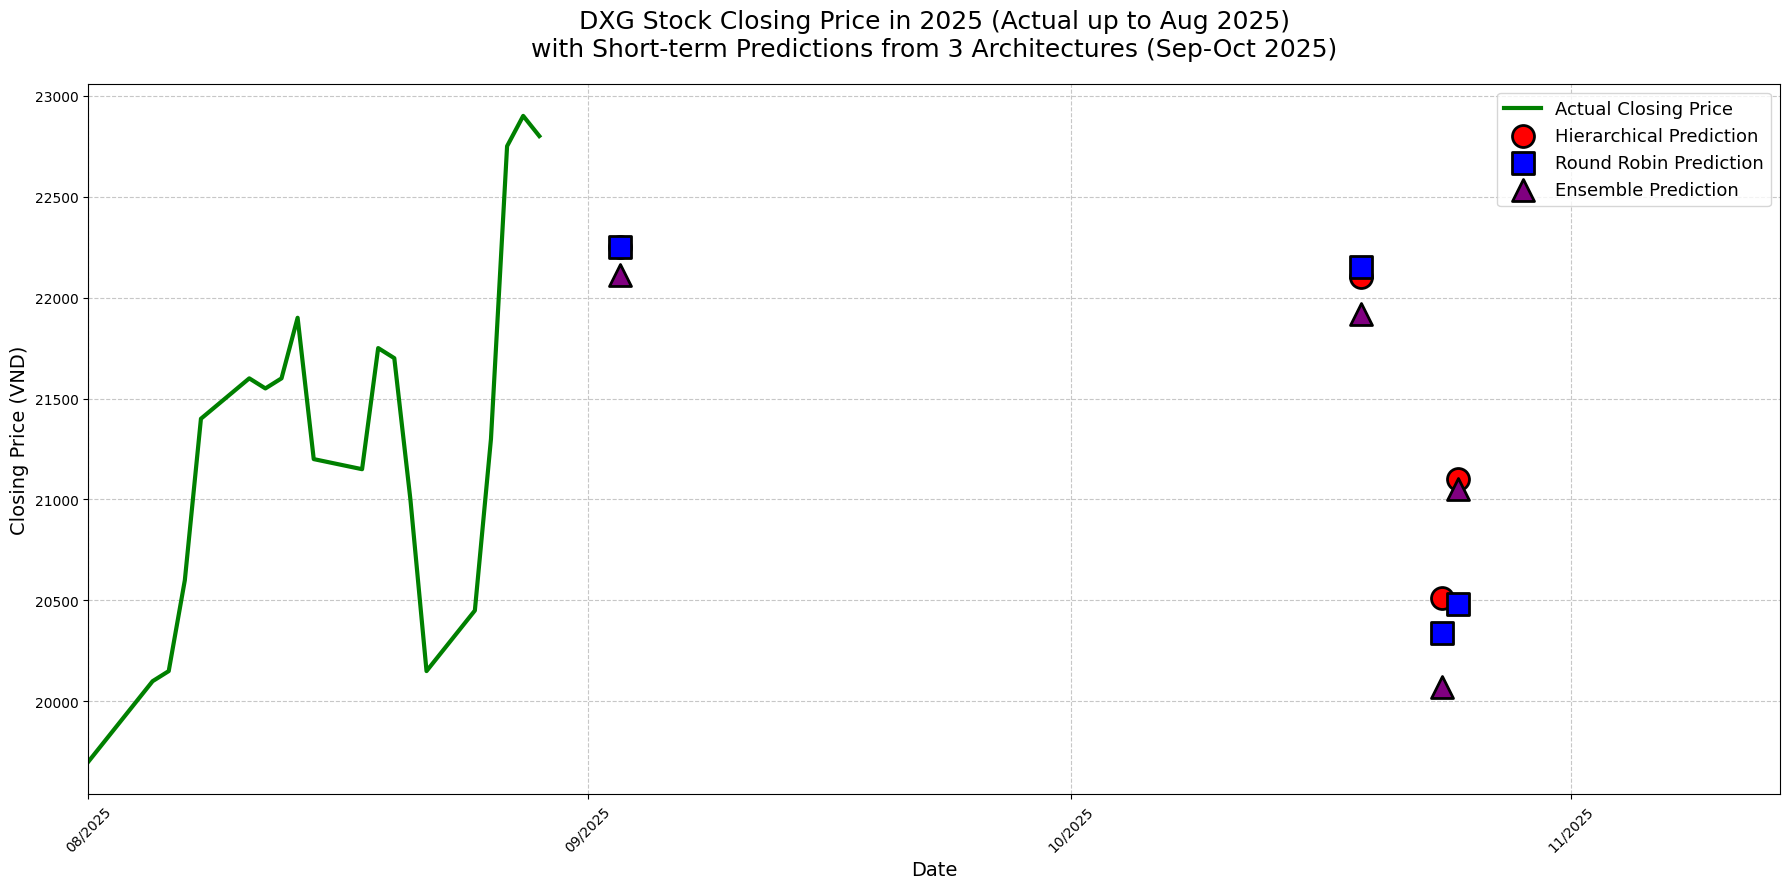
\includegraphics[width=\linewidth,height=3.5cm]{anh/main/dxg.png}
        \caption{DXG}
        \label{fig:short_dxg}
    \end{subfigure}
    \hfill
    \begin{subfigure}[b]{0.48\columnwidth}
        \centering
        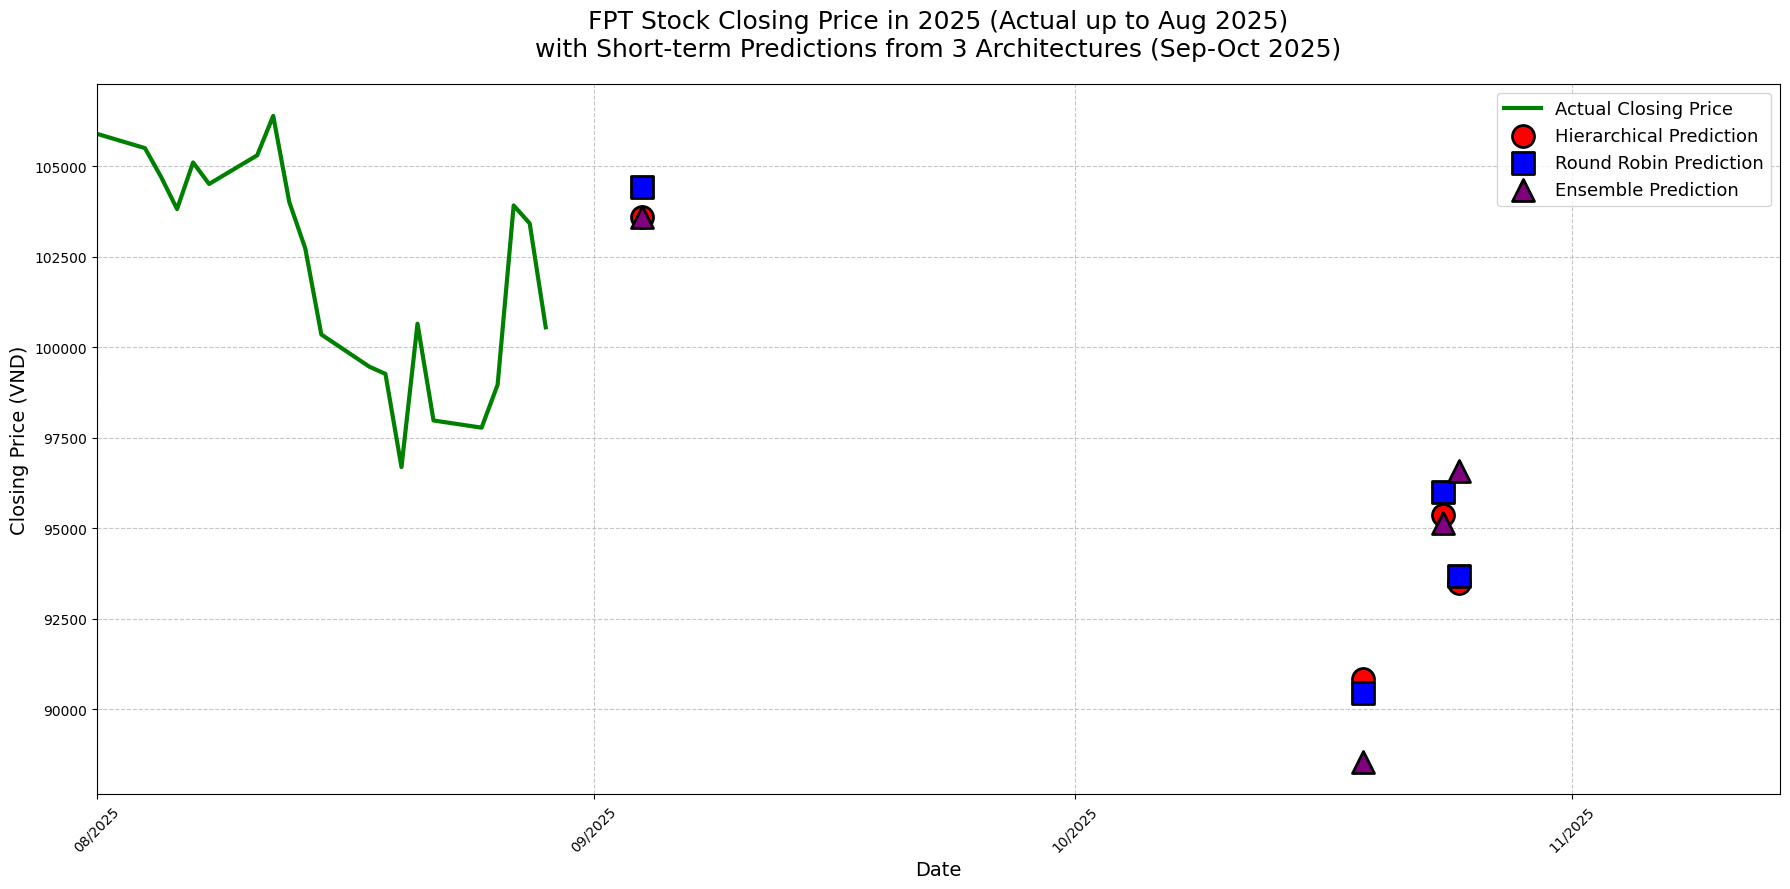
\includegraphics[width=\linewidth,height=3.5cm]{anh/main/fpt.png}
        \caption{FPT}
        \label{fig:short_fpt}
    \end{subfigure}

    \vspace{2mm}

    \begin{subfigure}[b]{0.48\columnwidth}
        \centering
        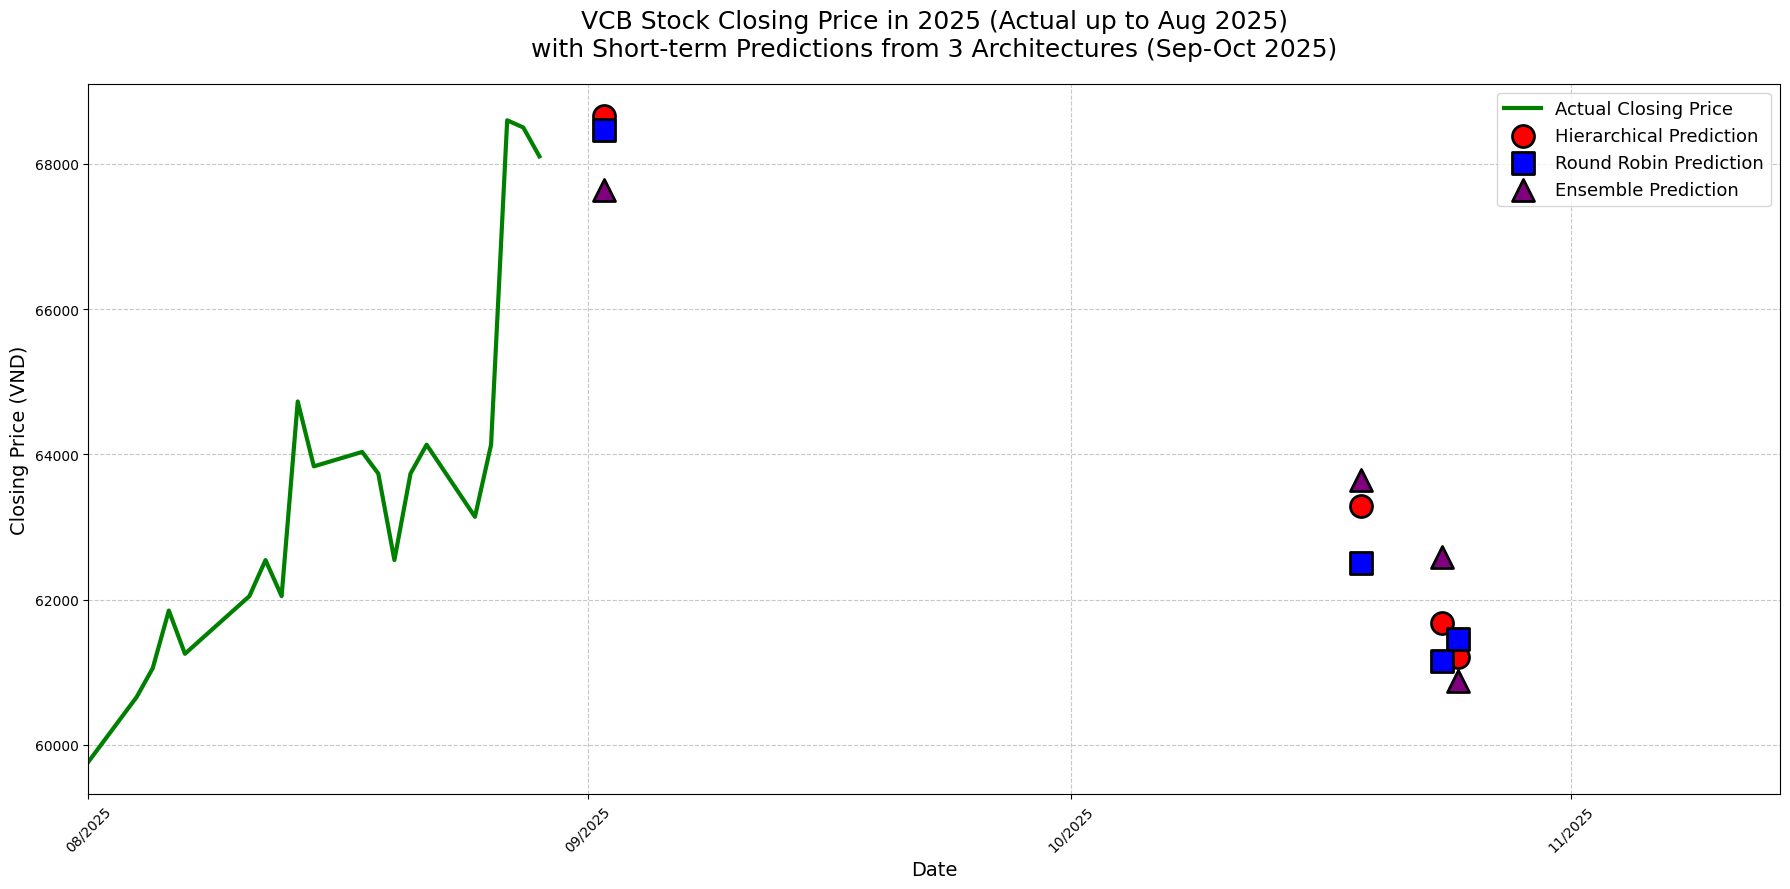
\includegraphics[width=\linewidth,height=3.5cm]{anh/main/vcb.png}
        \caption{VCB}
        \label{fig:short_vcb}
    \end{subfigure}
    \hfill
    \begin{subfigure}[b]{0.48\columnwidth}
        \centering
        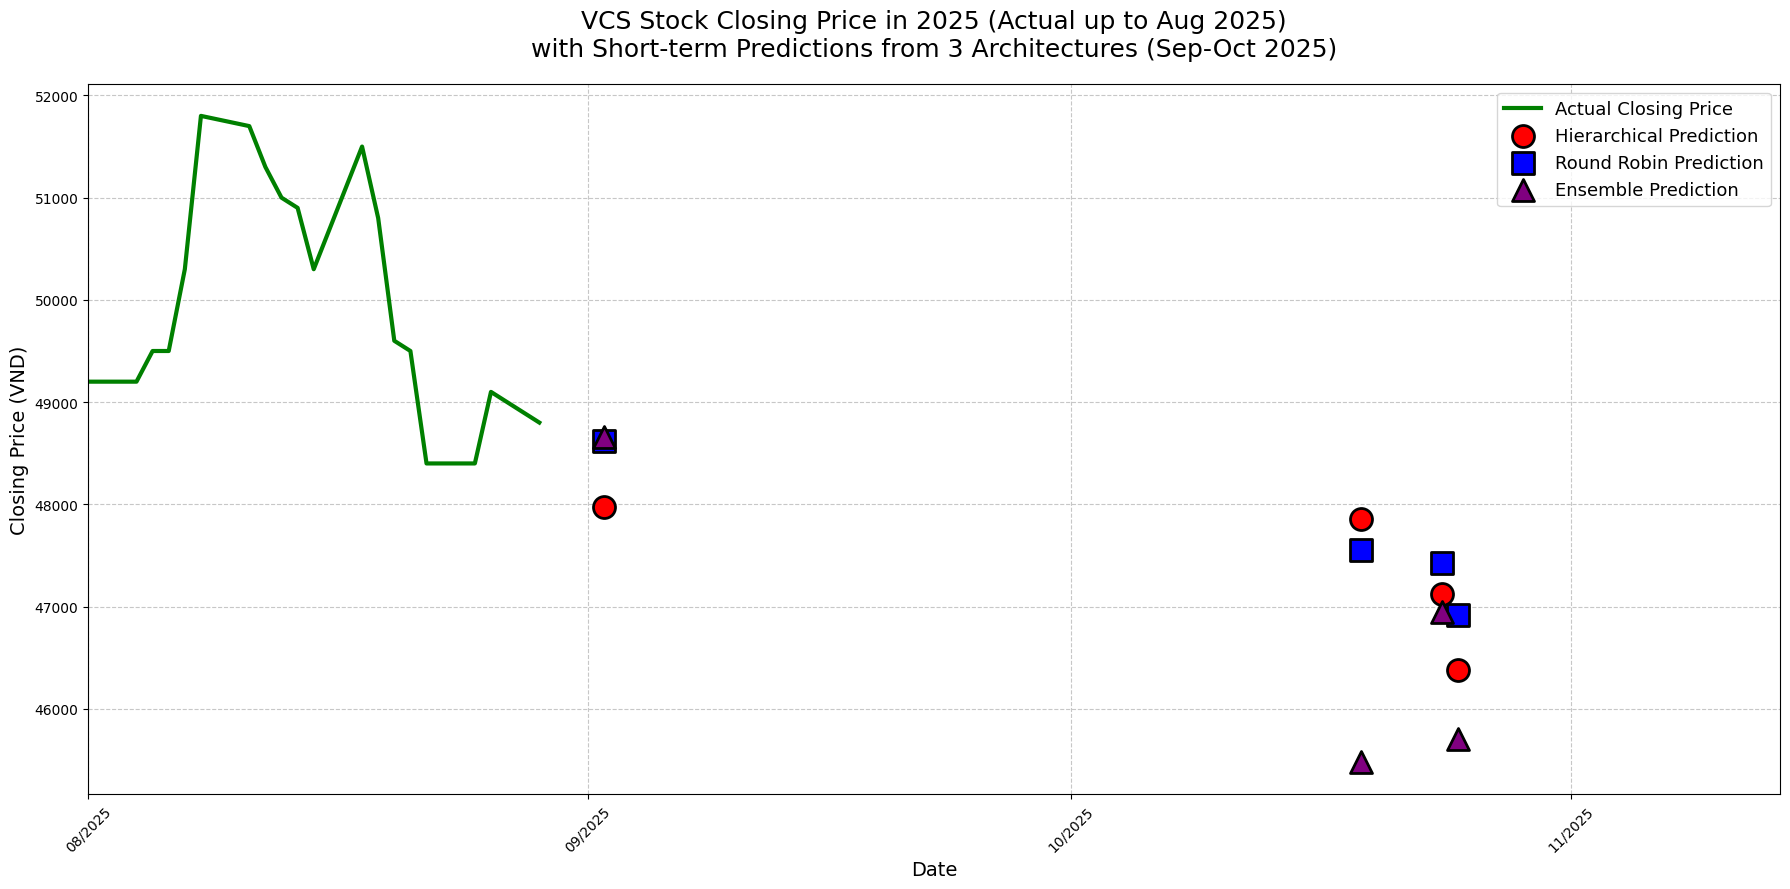
\includegraphics[width=\linewidth,height=3.5cm]{anh/main/vcs.png}
        \caption{VCS}
        \label{fig:short_vcs}
    \end{subfigure}
    
    \caption{Short-term Forecast Comparison Across Stocks}
    \label{fig:short_forecast_all}
\end{figure}

\begin{figure}[!h]
    \centering
    \begin{subfigure}[b]{0.48\columnwidth}
        \centering
        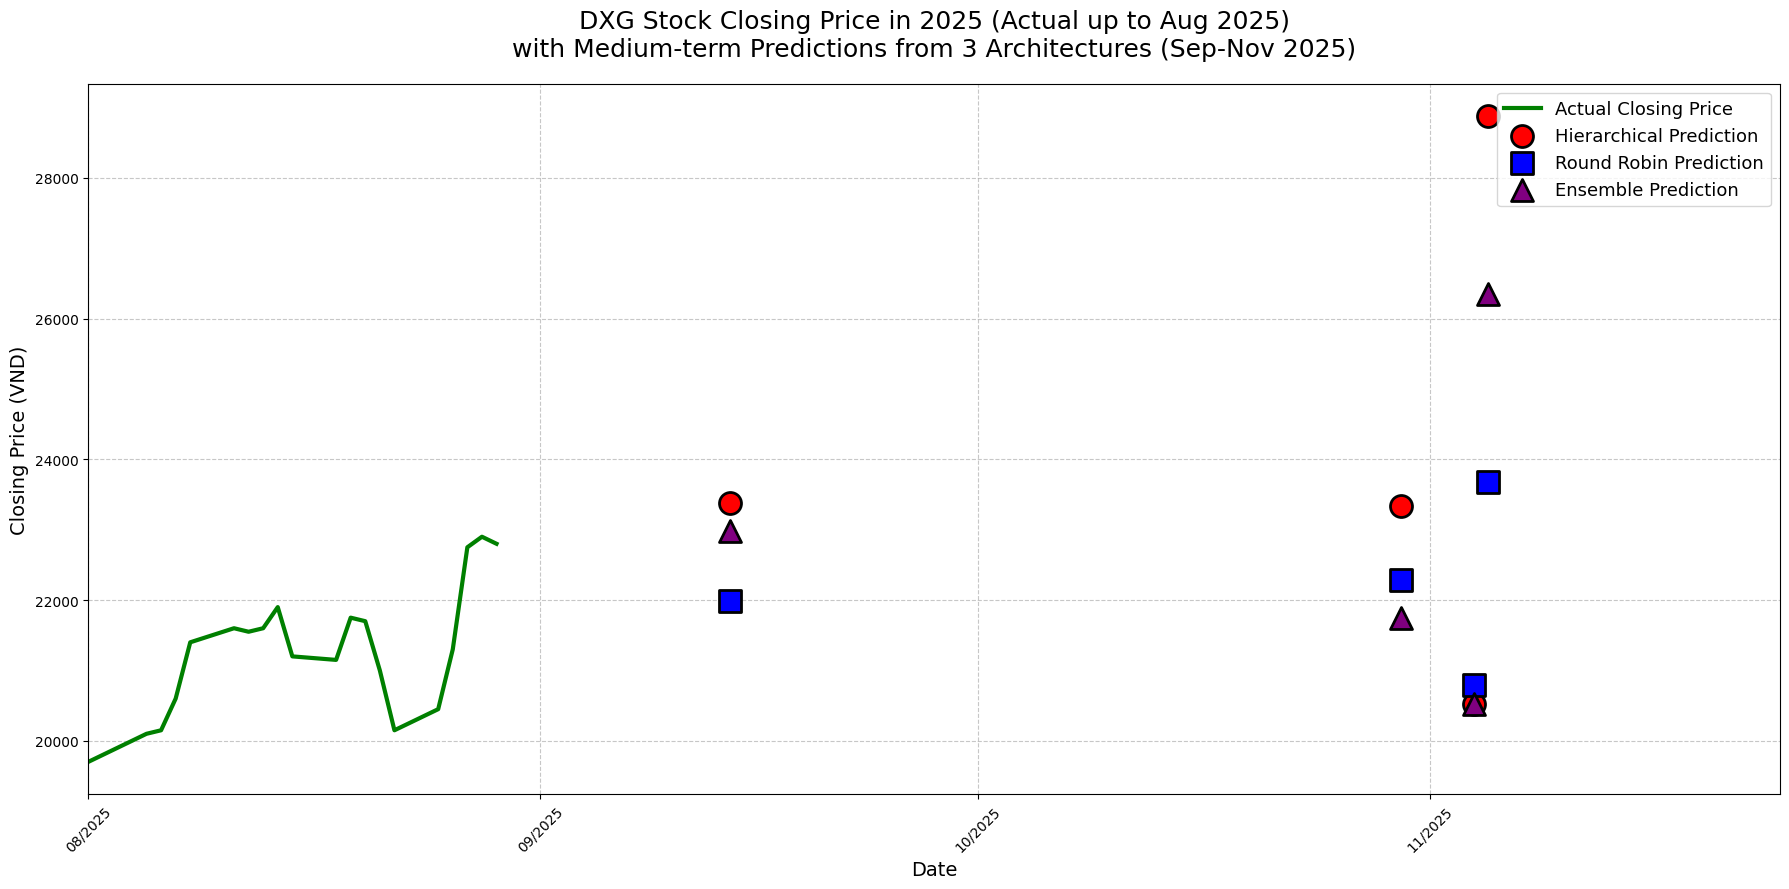
\includegraphics[width=\linewidth,height=3.5cm]{anh/main/dxgmedium.png}
        \caption{DXG}
        \label{fig:medium_dxg}
    \end{subfigure}
    \hfill
    \begin{subfigure}[b]{0.48\columnwidth}
        \centering
        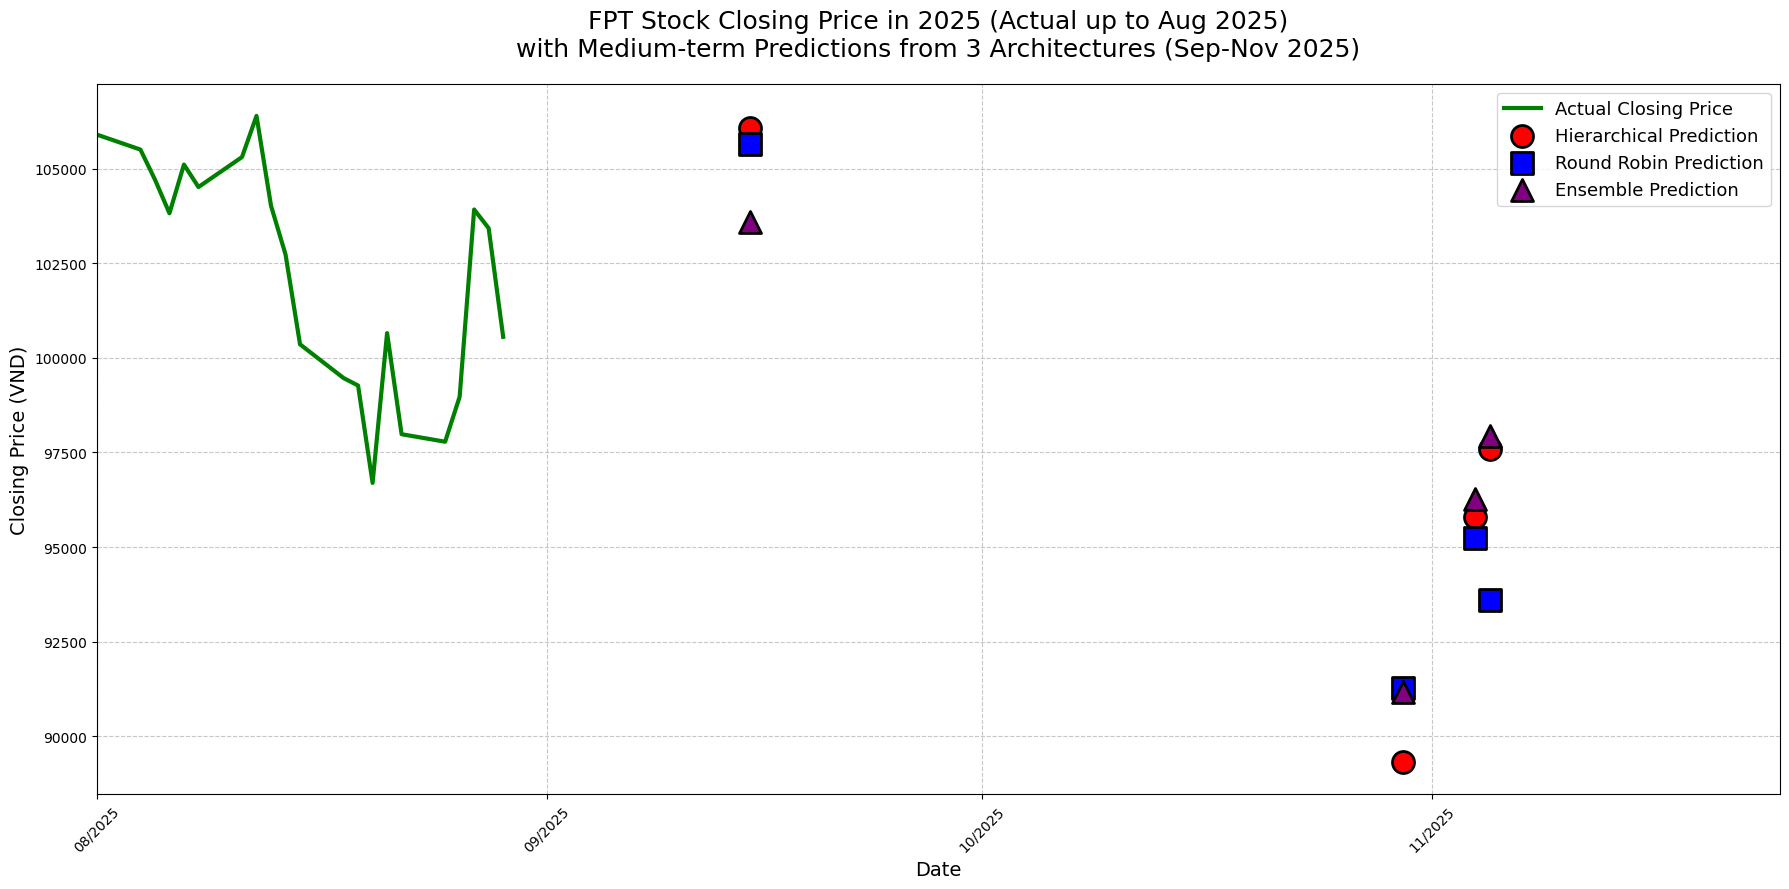
\includegraphics[width=\linewidth,height=3.5cm]{anh/main/fptmedium.png}
        \caption{FPT}
        \label{fig:medium_fpt}
    \end{subfigure}

    \vspace{2mm}

    \begin{subfigure}[b]{0.48\columnwidth}
        \centering
        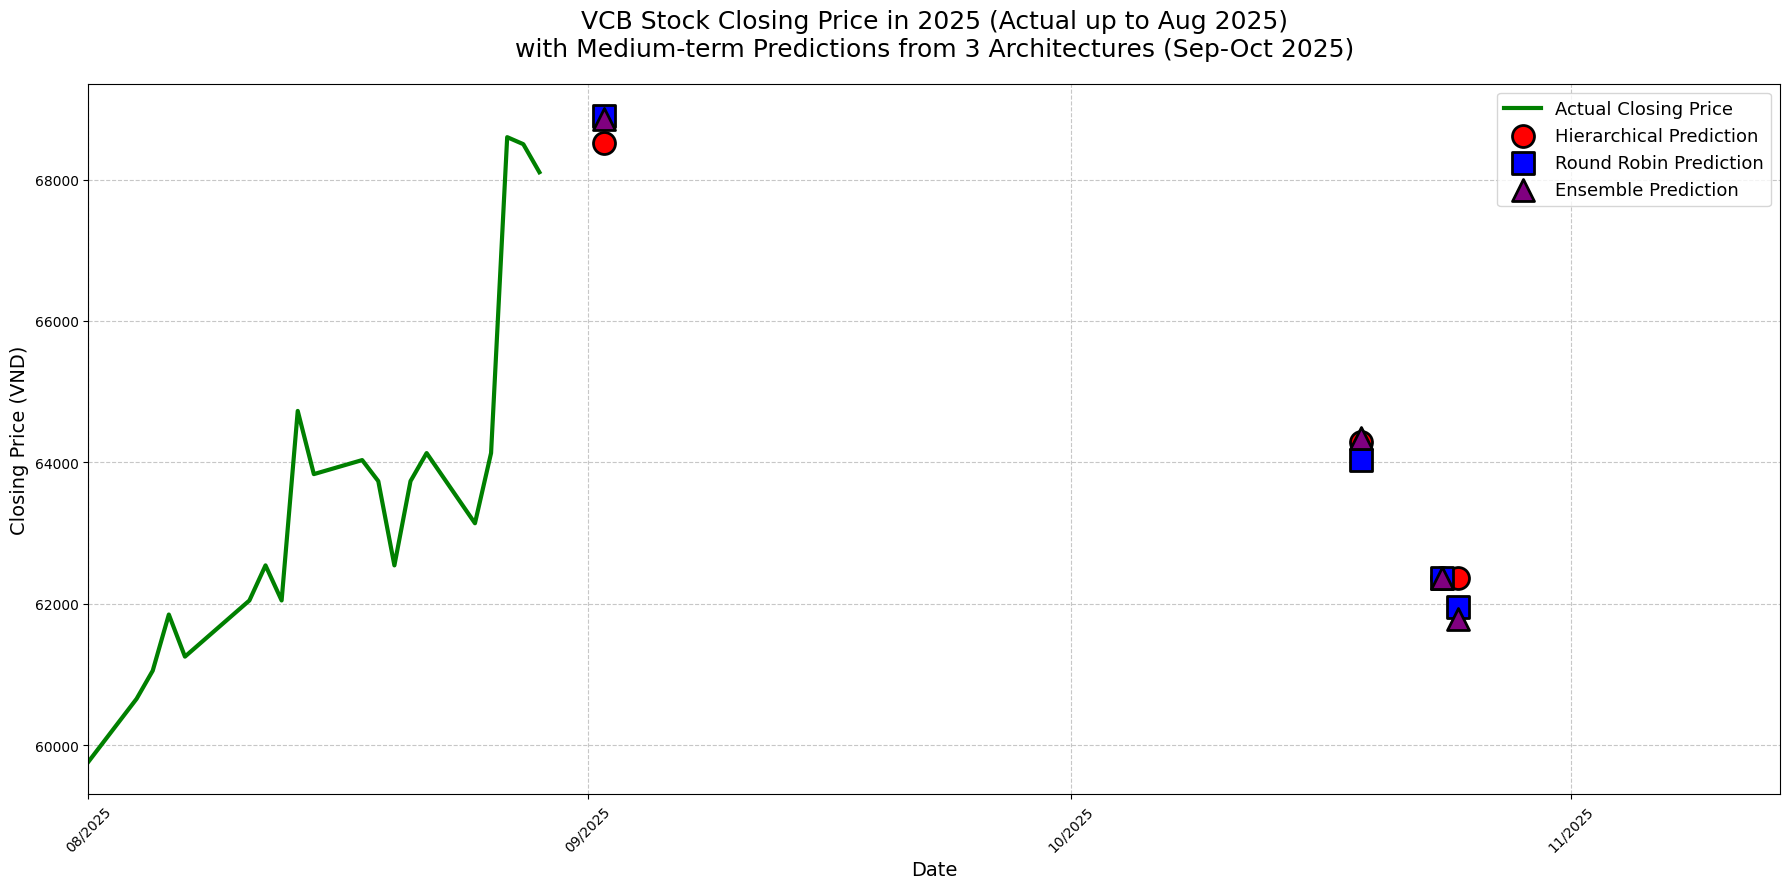
\includegraphics[width=\linewidth,height=3.5cm]{anh/main/vcbmedium.png}
        \caption{VCB}
        \label{fig:medium_vcb}
    \end{subfigure}
    \hfill
    \begin{subfigure}[b]{0.48\columnwidth}
        \centering
        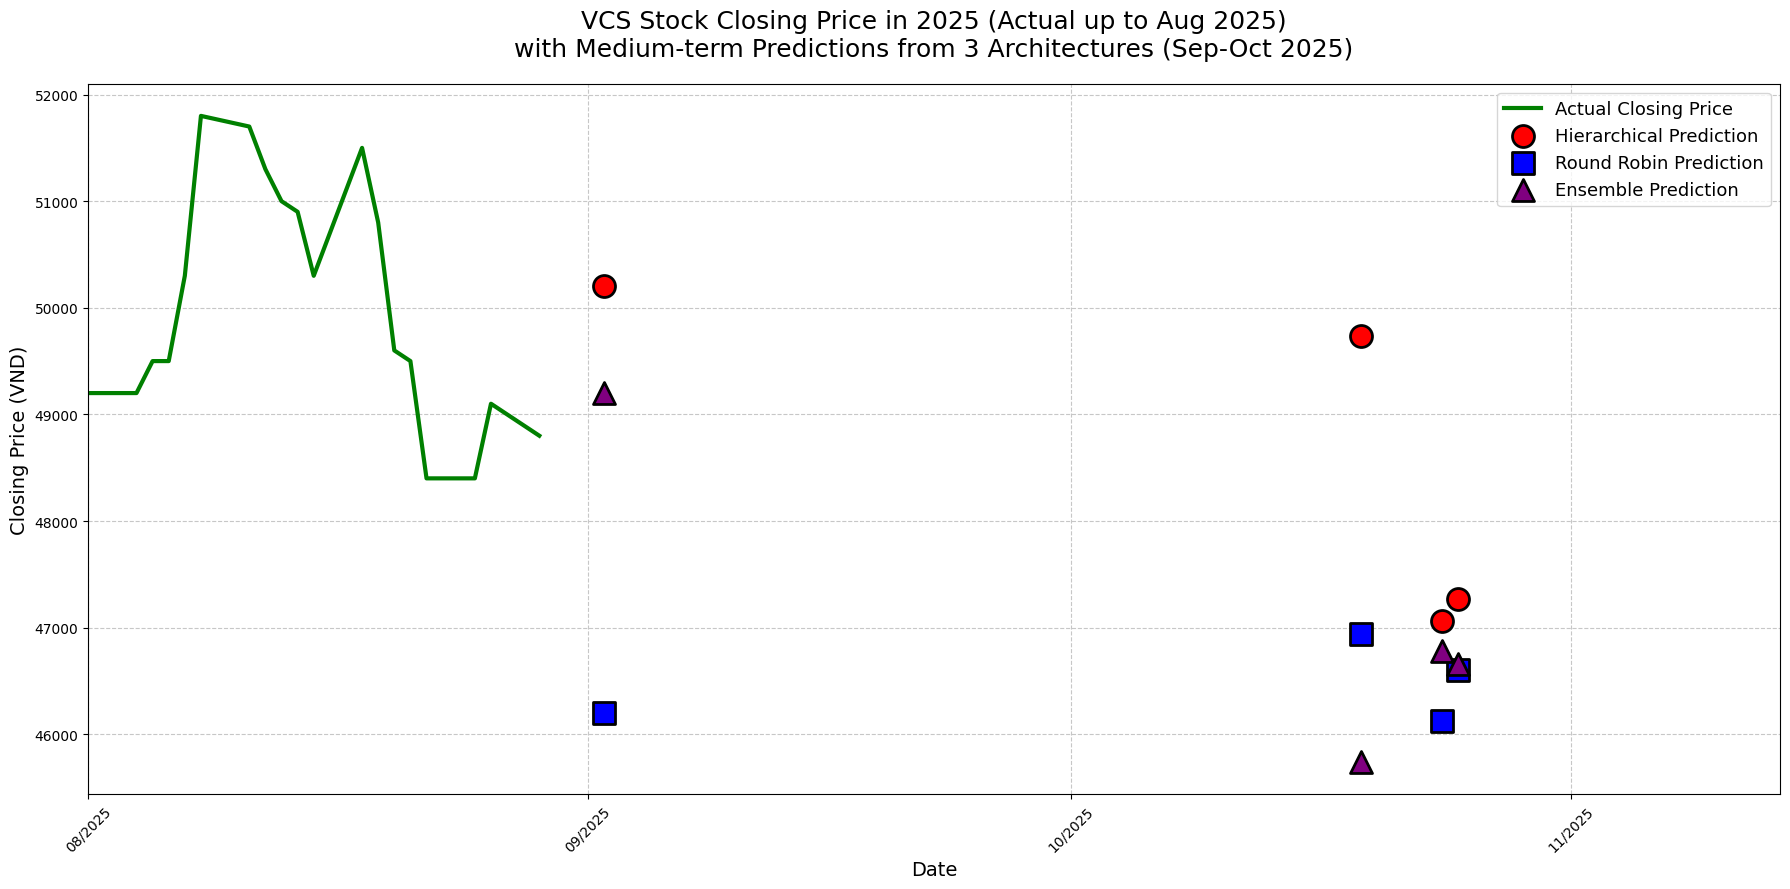
\includegraphics[width=\linewidth,height=3.5cm]{anh/main/vcsmedium.png}
        \caption{VCS}
        \label{fig:medium_vcs}
    \end{subfigure}
    
    \caption{Medium-term Forecast Comparison Across Stocks}
    \label{fig:medium_forecast_all}
\end{figure}
\newpage
\begin{figure}[!h]
    \centering
    \begin{subfigure}[b]{0.48\columnwidth}
        \centering
        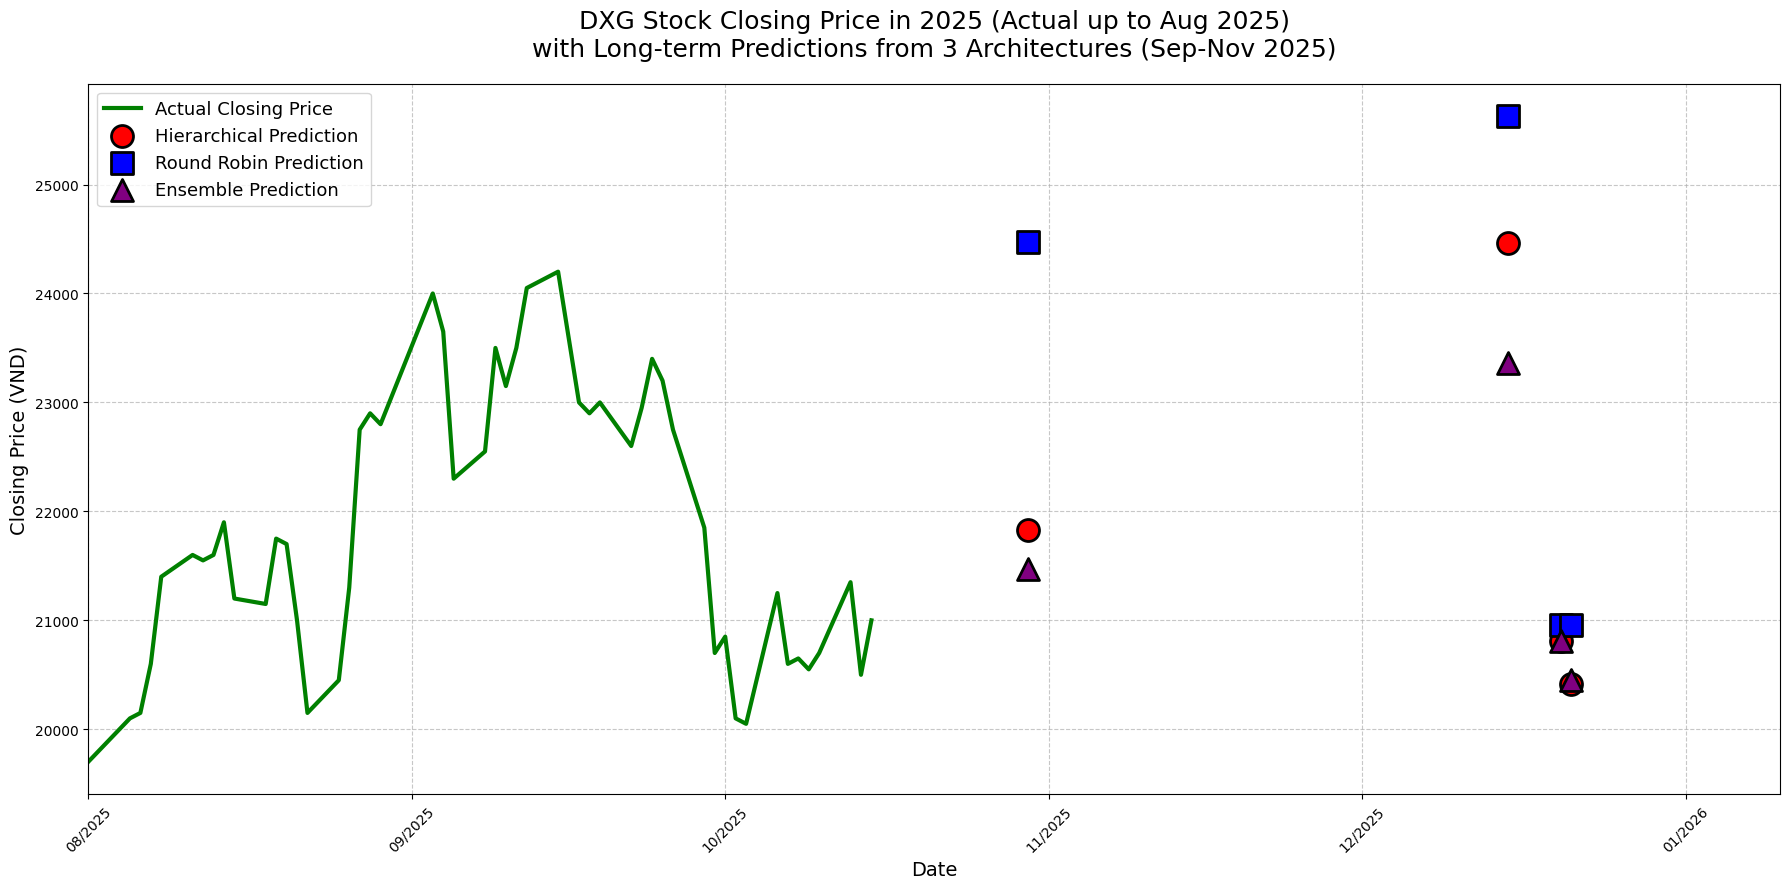
\includegraphics[width=\linewidth,height=3.5cm]{anh/main/dxglong.png}
        \caption{DXG}
        \label{fig:long_dxg}
    \end{subfigure}
    \hfill
    \begin{subfigure}[b]{0.48\columnwidth}
        \centering
        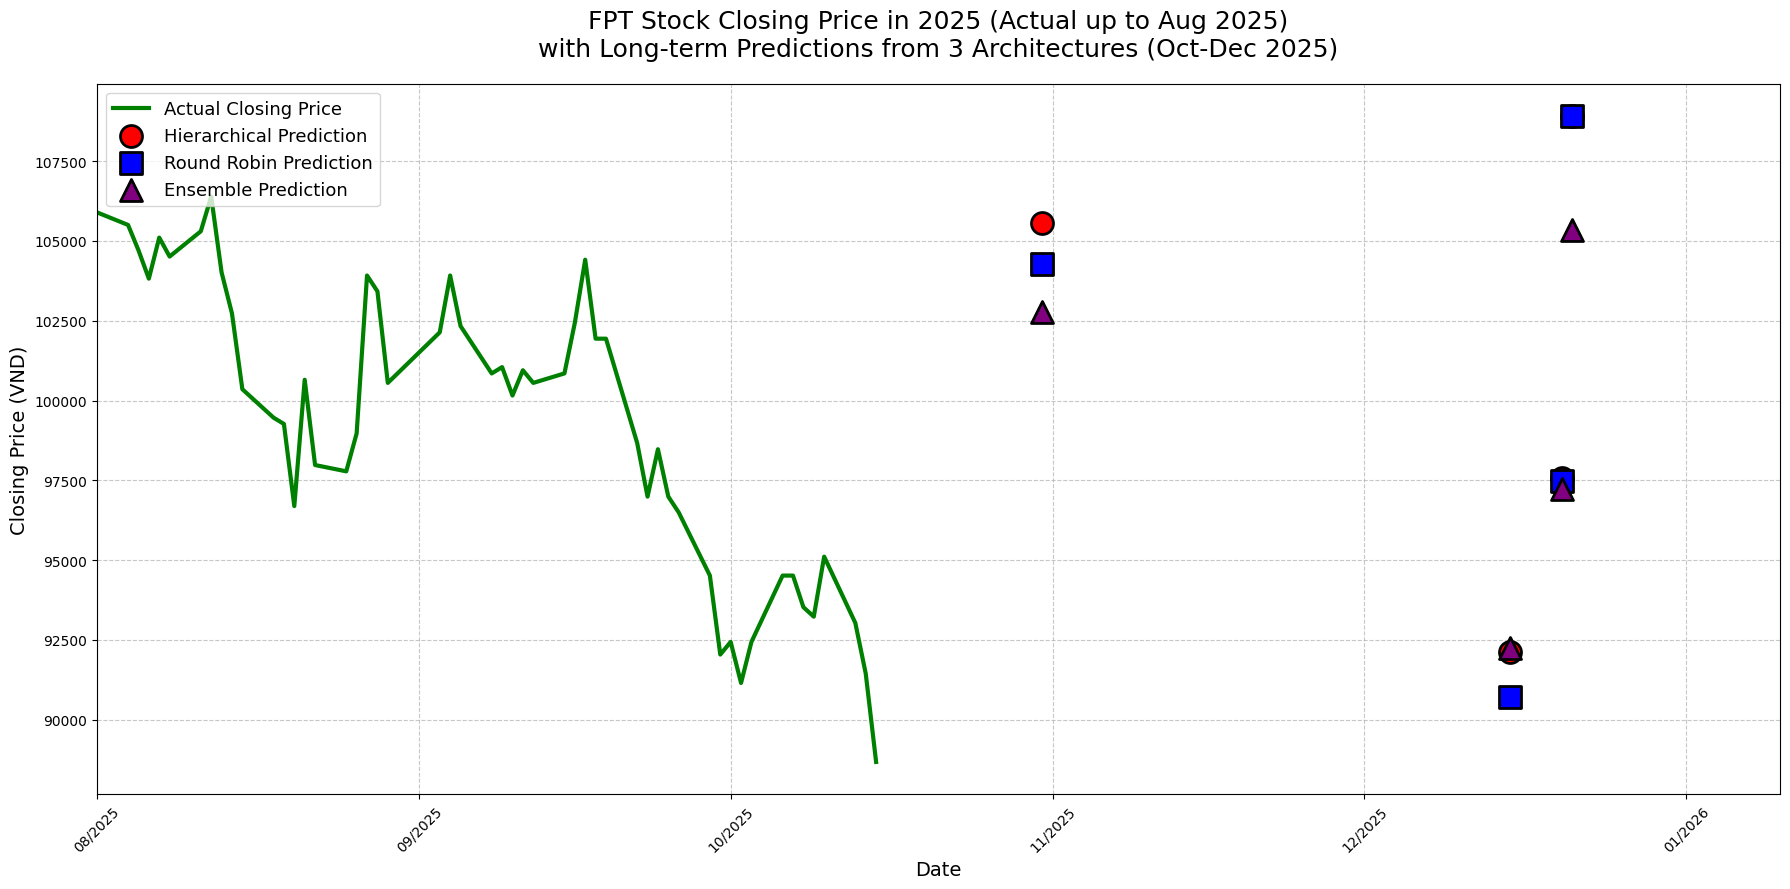
\includegraphics[width=\linewidth,height=3.5cm]{anh/main/fptlong.png}
        \caption{FPT}
        \label{fig:long_fpt}
    \end{subfigure}

    \vspace{2mm}

    \begin{subfigure}[b]{0.48\columnwidth}
        \centering
        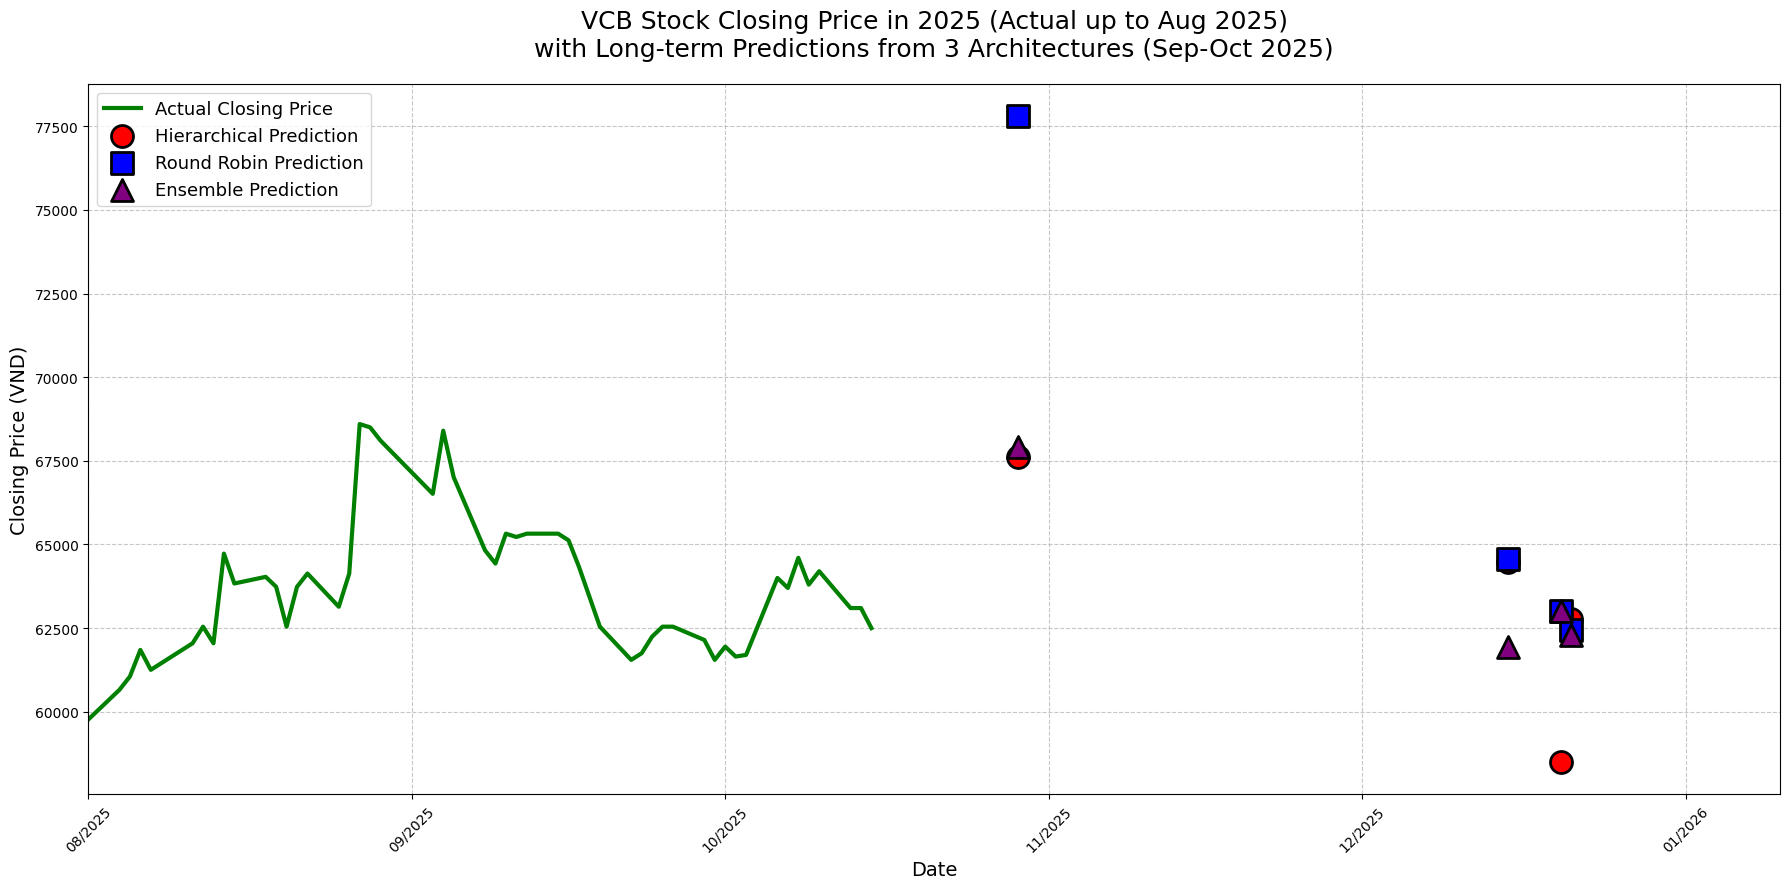
\includegraphics[width=\linewidth,height=3.5cm]{anh/main/vcblong.png}
        \caption{VCB}
        \label{fig:long_vcb}
    \end{subfigure}
    \hfill
    \begin{subfigure}[b]{0.48\columnwidth}
        \centering
        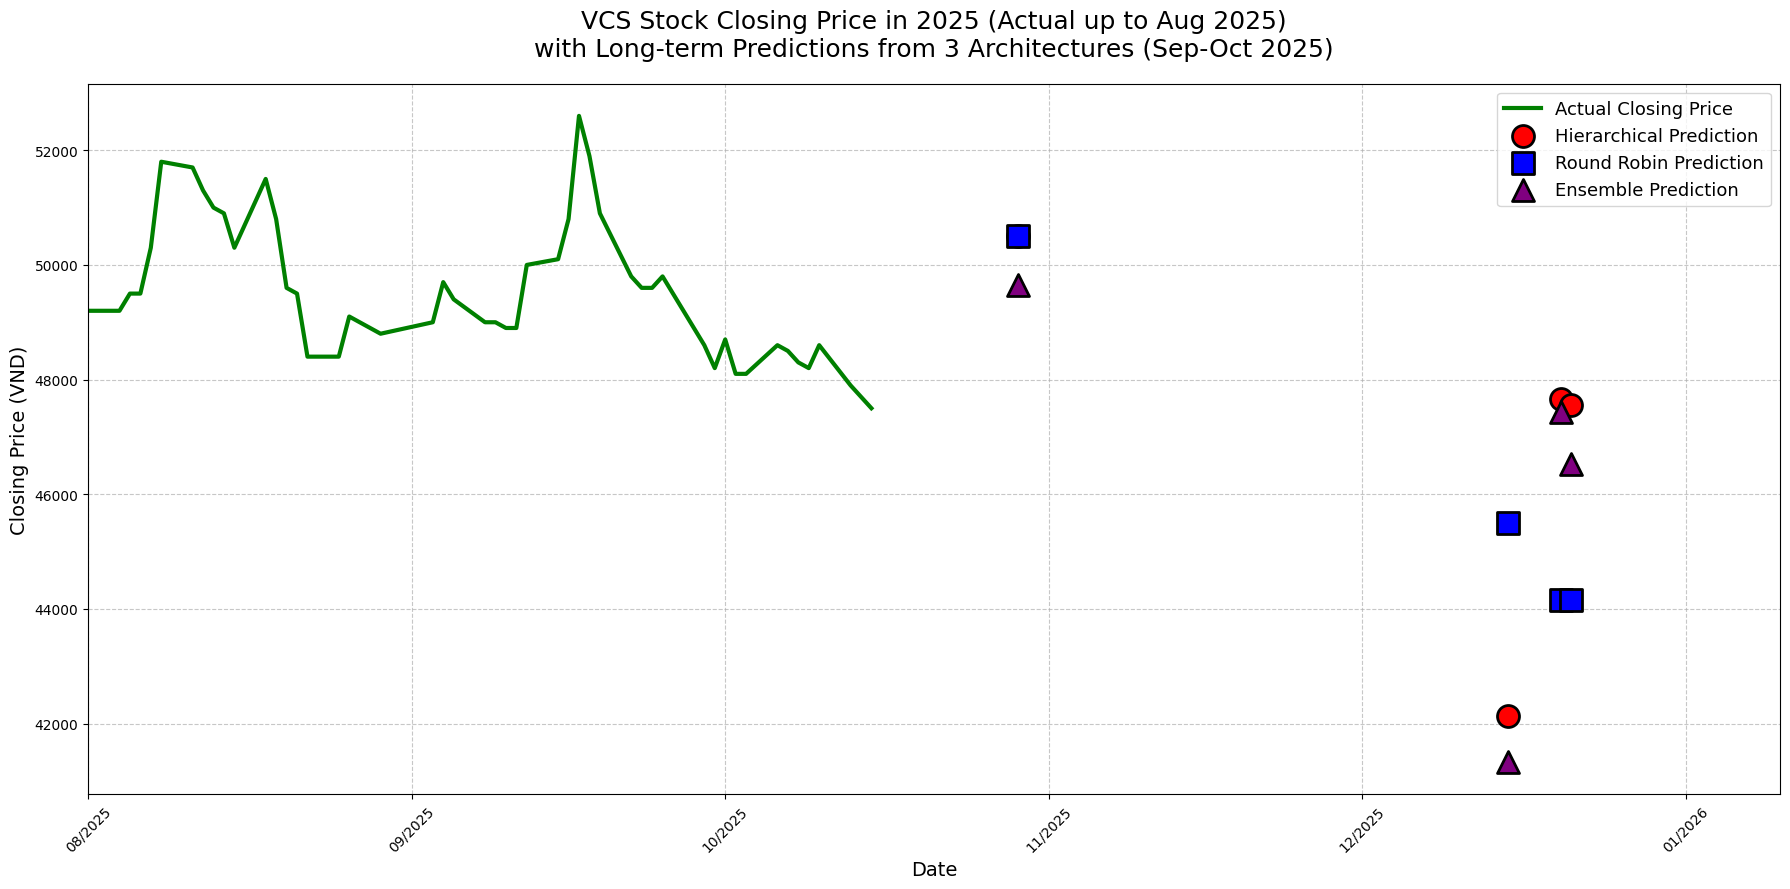
\includegraphics[width=\linewidth,height=3.5cm]{anh/main/vcslong.png}
        \caption{VCS}
        \label{fig:long_vcs}
    \end{subfigure}
    
    \caption{Long-term Forecast Comparison Across Stocks}
    \label{fig:long_forecast_all}
\end{figure}

\section{Multi-Agent vs. Single-Agent vs Machine Learning Baseline(RQ2)}
To address RQ2, we present a comprehensive comparison framework between multi-agent coordination architectures, single-agent approaches, and baseline machine learning models. The evaluation focuses on medium-term (14-day) forecasting capabilities across the four selected Vietnamese stocks, demonstrating the different methodological approaches and their respective prediction outputs.

\begin{figure}[H]
    \centering
    \begin{subfigure}[b]{0.48\columnwidth}
        \centering
        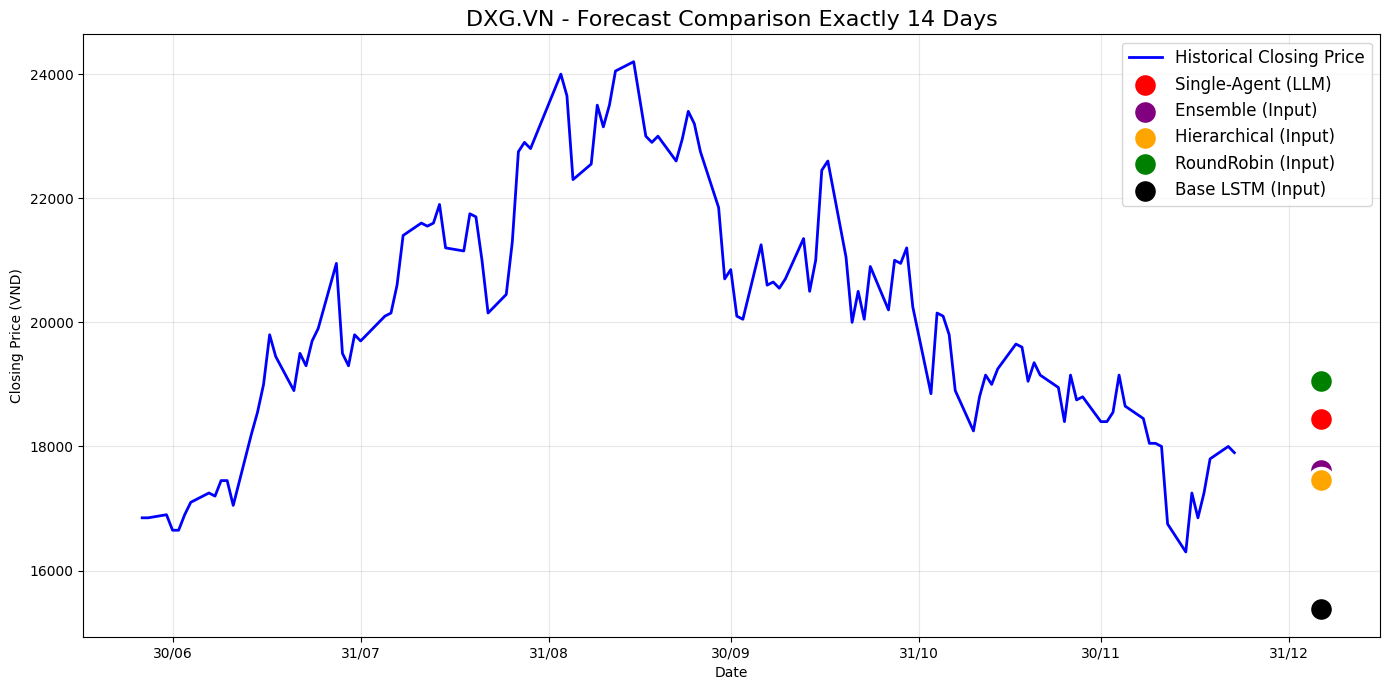
\includegraphics[width=\linewidth,height=3.2cm]{anh/new/dxgrq2main.png}
        \caption{DXG}
        \label{fig:single_dxg}
    \end{subfigure}
    \hfill
    \begin{subfigure}[b]{0.48\columnwidth}
        \centering
        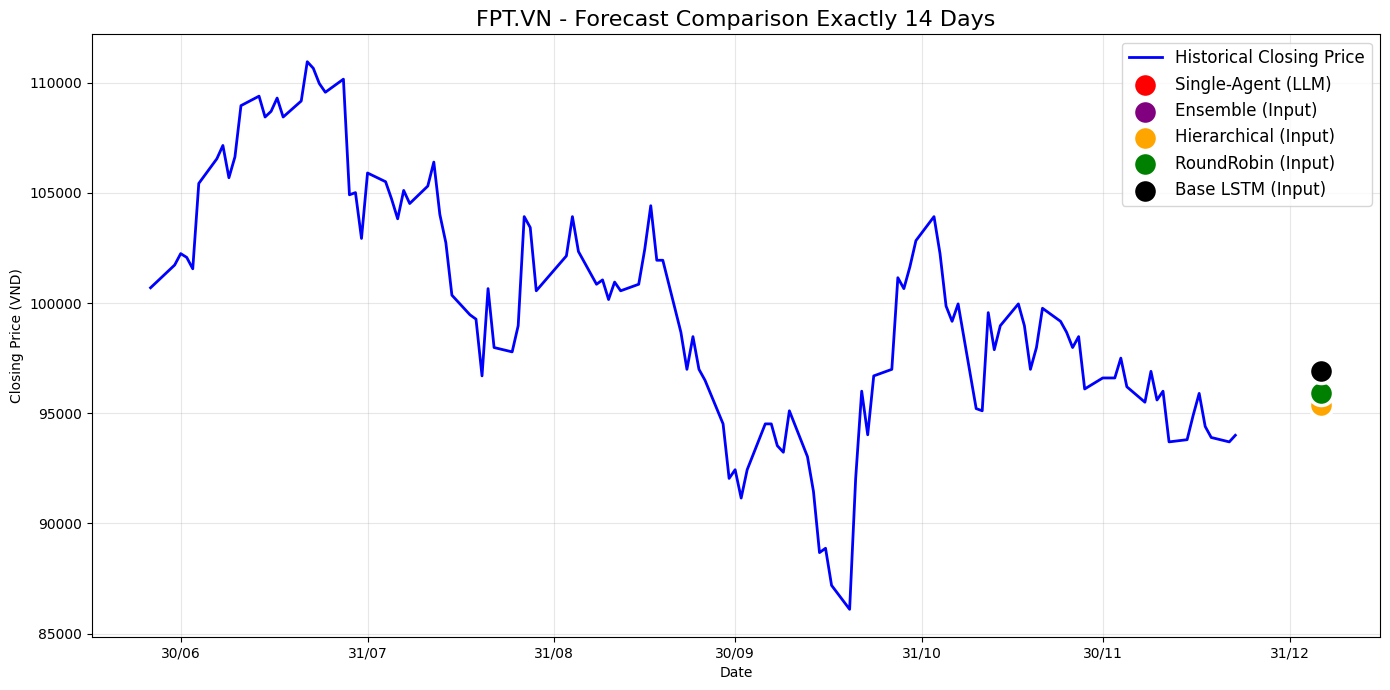
\includegraphics[width=\linewidth,height=3.2cm]{anh/new/fptrq2main.png}
        \caption{FPT}
        \label{fig:single_fpt}
    \end{subfigure}

    \vspace{2mm}

    \begin{subfigure}[b]{0.48\columnwidth}
        \centering
        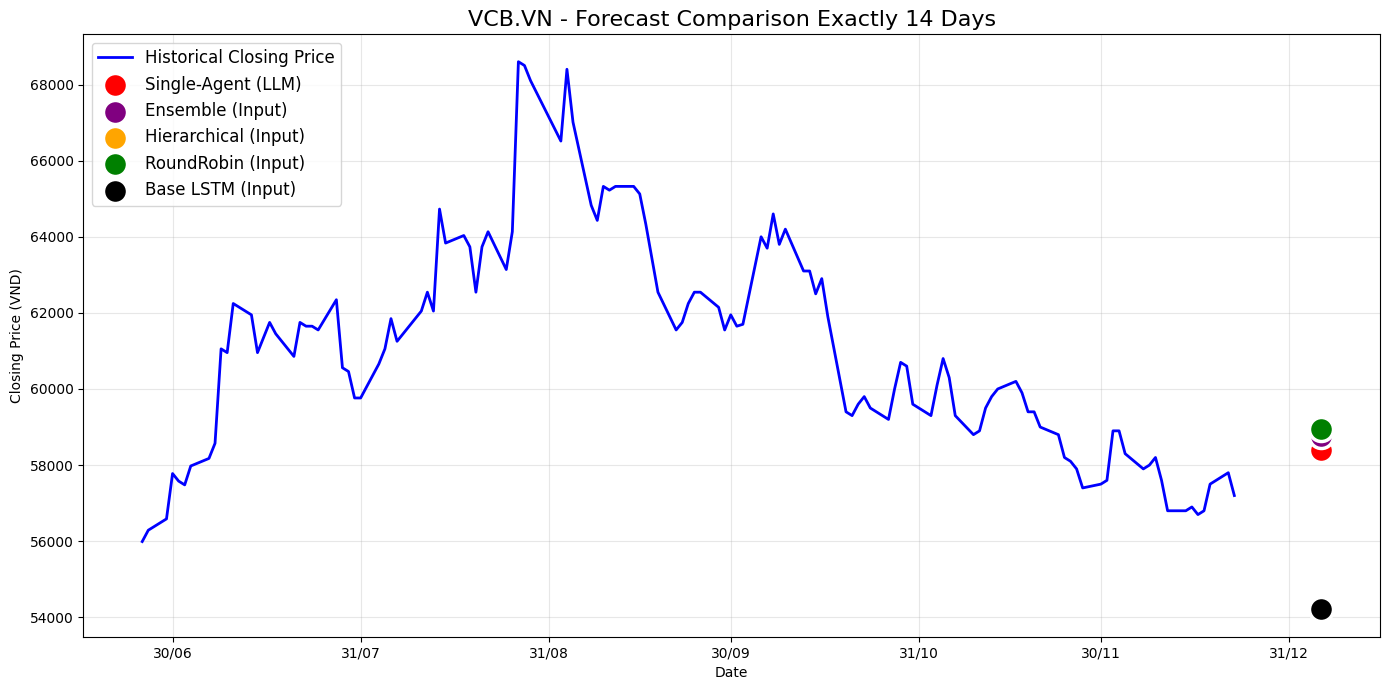
\includegraphics[width=\linewidth,height=3.2cm]{anh/new/vcbrq2main.png}
        \caption{VCB}
        \label{fig:single_vcb}
    \end{subfigure}
    \hfill
    \begin{subfigure}[b]{0.48\columnwidth}
        \centering
        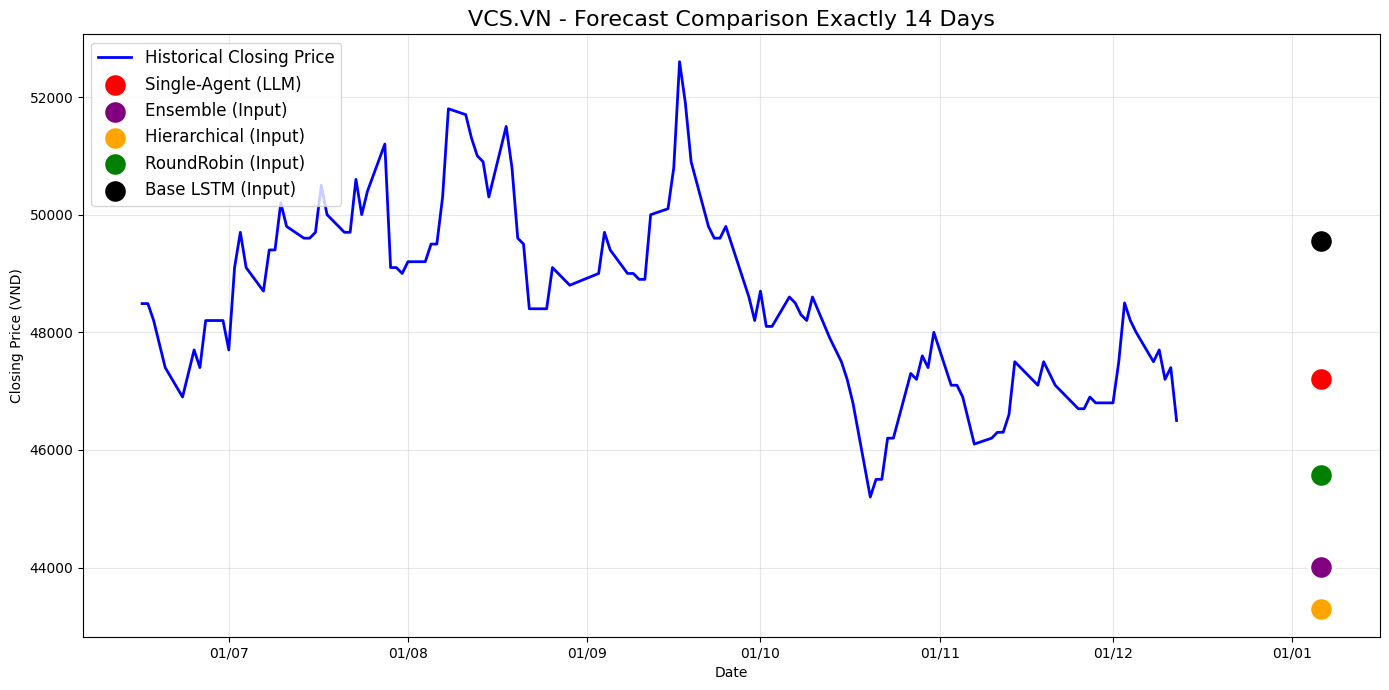
\includegraphics[width=\linewidth,height=3.2cm]{anh/new/vcsrq2main.png}
        \caption{VCS}
        \label{fig:single_vcs}
    \end{subfigure}

    \caption{Comparative Framework: 14-day Forecasting Results Across Different Approaches}
    \label{fig:single_agent_2x2}
\end{figure}

\subsection{Methodological Comparison Framework and Visual Analysis}

\subsubsection{Methodological Comparison Framework}
This study establishes a systematic comparative framework to evaluate three forecasting methodologies characterized by distinct architectural principles. By mapping point forecasts—represented as discrete markers in the visual results—against historical closing prices (blue line), we assess the robustness and behavioral characteristics of each approach. This visual juxtaposition enables a granular analysis of predictive accuracy and model stability under varying market conditions, providing empirical insights into each architecture's adaptability to market volatility and its utility for practical decision-making.

\subsubsection{Multi-Agent Coordination Architectures}
The multi-agent systems—distinguished by green (Round Robin), orange (Hierarchical), and purple (Ensemble Voting) markers—demonstrate distinct emergent behaviors derived from their respective coordination protocols. These architectures utilize sophisticated interaction mechanisms to process heterogeneous data streams, aiming to enhance prediction stability amidst market volatility.

\paragraph{Behavioral Clustering.}
Visual analysis of the DXG and FPT forecasts reveals a strong convergence between the Hierarchical (orange) and Ensemble Voting (purple) architectures. This clustering suggests that the centralized aggregation and voting mechanisms effectively function as a low-pass filter, mitigating the idiosyncratic variances produced by individual agents and converging toward a stable consensus.

\paragraph{Architecture-Specific Traits.}
Conversely, the Round Robin architecture (green marker) exhibits a persistent \textit{optimistic bias}. In high-variance scenarios such as DXG and VCB, this architecture generates predictions significantly above the realized closing price (e.g., $\approx$ 19,000 VND for DXG versus the actual 16,300 VND). This suggests that the sequential refinement process may suffer from cumulative error propagation, leading to "overshooting" during bearish trend reversals.

In contrast, the Ensemble Voting (purple) and Hierarchical (orange) architectures display superior \textit{moderation and noise resilience}. During the volatility spike in DXG, these architectures successfully dampened the Round Robin’s aggressive optimism and the LSTM’s extreme pessimism, aligning more closely with the intrinsic market valuation ($\approx$ 17,500 VND).

\subsubsection{Single-Agent Approach}
The Single-Agent methodology (red marker), leveraging the Large Language Model's reasoning capabilities without specialized sub-agent coordination, occupies an intermediate performance tier between the multi-agent consensus and the baseline model.

\paragraph{Performance in Stable Regimes.}
In stable market conditions like VCS, the Single-Agent approach demonstrates competitive efficacy. The prediction ($\approx$ 47,200 VND) aligns closely with the historical close ($\approx$ 46,500 VND), effectively outperforming the overly conservative estimates of the ensemble models. This indicates the foundation model's inherent capacity for fundamental value recognition in low-volatility contexts.

\paragraph{Structural Limitations.}
However, the absence of an error-correction mechanism becomes evident in volatile stocks like DXG and VCB. The Single-Agent model exhibits \textit{lag-induced inertia}, failing to adapt promptly to sharp corrections. For instance, in VCB, the forecast remains elevated at $\approx$ 58,400 VND despite the actual price dropping to 57,200 VND, highlighting a deficiency in detecting rapid regime shifts compared to the multi-agent consensus.

\subsubsection{Machine Learning Baseline (LSTM)}
The baseline LSTM model (black marker) serves as the control variable, exhibiting the highest degree of stochastic instability.

\paragraph{Stochastic Divergence.}
Across all evaluated equities, the LSTM frequently manifests as a statistical outlier, lacking the semantic grounding of LLM-based approaches.

\paragraph{Amplitude Distortion.}
The model demonstrates an inability to gauge magnitude correctly, resulting in significant \textit{undershooting} in downtrends (e.g., predicting a collapse to $\approx$ 15,400 VND for DXG) and pronounced \textit{overshooting} in uptrends (e.g., projecting a surge to $\approx$ 49,500 VND for VCS). This behavior reflects the model's sensitivity to local temporal noise rather than fundamental market drivers.

\subsubsection{Prediction Pattern Analysis}
The divergence patterns between predicted markers and historical trajectories offer critical insights into the interplay between model architecture and market entropy.

\paragraph{Sector-Specific Volatility and Model Uncertainty.}
The dispersion of predictions is strongly correlated with sector volatility. The DXG chart (Real Estate) displays maximum uncertainty, with forecasts spanning a wide range from $\approx$ 15,400 VND (LSTM) to 19,000 VND (Round Robin). Conversely, the FPT chart (Technology) shows tight clustering within the 95,000--97,000 VND band, indicating that model uncertainty scales with the inherent instability of the underlying asset class.

\paragraph{Ensemble as a Stability Anchor.}
The Ensemble Voting (purple) and Hierarchical (orange) architectures consistently avoid the boundary conditions of the forecast distribution. By rejecting the extremes exhibited by the LSTM (black) and Round Robin (green), these architectures function as a \textit{stability anchor}, prioritizing risk minimization over aggressive directional bets.

\paragraph{Trend Alignment.}
While the Single-Agent model (red) adequately captures general price levels, it struggles with the precise timing of trend reversals. Multi-agent architectures—specifically Ensemble Voting—demonstrate superior \textit{tactical alignment}, leveraging diverse agent perspectives to identify turning points more accurately than single-model approaches.

\subsection{Conclusion}
Empirical evidence from the visual trajectory analysis validates the hypothesis that multi-agent coordination provides a superior robustness profile compared to standalone baselines. While the Single-Agent approach offers a viable, low-latency solution for stable assets (e.g., VCS), it lacks the resilience required for volatile environments (e.g., DXG). Critically, the LSTM baseline is proven unsuitable for reliable decision support due to its susceptibility to extreme amplitude distortion. Consequently, the \textbf{Ensemble Voting architecture} is established as the optimal configuration, effectively balancing sensitivity to market signals with the stability necessary for actionable financial forecasting in Vietnam's emerging market.

\section{Discussion}
\subsection{Key Findings and Implications}
This study presents several significant findings that advance our understanding of multi-agent coordination architectures in financial forecasting, particularly within emerging market contexts. The empirical evaluation reveals that coordination architecture effectiveness exhibits strong horizon-dependent characteristics, with Ensemble Voting demonstrating consistent superiority across three of the four evaluated stocks in medium-term forecasting scenarios (outperforming significantly in FPT and VCS, and showing comparable performance in VCB).

The superior performance of Ensemble Voting in medium-term forecasting can be attributed to its statistical inference mechanism that dynamically aggregates diverse analytical perspectives while maintaining robustness against individual agent biases~\cite{zhou2012ensemble,breiman1996bagging}. Our results show that Ensemble Voting achieves highly competitive MAPE in the 14-day horizon: DXG (10.0\%), FPT (5.7\%), VCB (4.0\%), and VCS (1.6\%), securing the lowest error in FPT, VCS, and jointly in VCB (where values are virtually indistinguishable across architectures). This strong consistency validates ensemble learning theory, which posits that combining multiple specialized learners can produce superior generalization capabilities compared to individual models~\cite{dietterich2000ensemble}.
For Vietnam's retail-dominated market structure, these findings carry substantial practical implications for institutional investment strategies and risk management frameworks~\cite{vo2019financial,nguyen2021market}. The framework's demonstrated ability to handle sentiment-driven volatility and information asymmetries makes it particularly valuable for emerging market applications where traditional fundamental analysis approaches may encounter limitations due to data quality and market efficiency constraints~\cite{bekaert2007emerging}. The consistent performance across diverse sectors (banking, technology, real estate, and industrial construction) suggests broad applicability within Vietnam's financial ecosystem.

The horizon-dependent architectural effectiveness reveals critical insights about temporal market dynamics and optimal coordination strategies. Short-term predictions (3-day horizon) exhibit stock-specific architectural preferences, with no single architecture dominating across all securities. This heterogeneity suggests that rapid price movements are influenced by idiosyncratic factors requiring tailored analytical approaches~\cite{campbell1997stock}. Conversely, medium-term forecasting benefits from ensemble aggregation, indicating that tactical investment horizons are better served by comprehensive multi-perspective analysis that can capture both technical and fundamental market drivers.

Long-term predictions (60-day horizon) demonstrate mixed architectural preferences, with Hierarchical architecture proving optimal for VCB (8.9\% MAPE), while Ensemble Voting maintains advantages for DXG (19.1\% MAPE) and FPT (4.6\% MAPE), and Round Robin shows best performance for VCS (3.4\% MAPE). This redistribution possibly reflects the increased uncertainty and regime change probability inherent in extended forecasting horizons, where centralized coordination may provide stability for certain market segments while ensemble approaches remain effective for others~\cite{guidolin2007asset}.

The integration of Large Language Models with specialized financial agents represents a significant methodological advancement in computational finance. The LLM's natural language processing capabilities enable sophisticated interpretation of unstructured information sources—news sentiment, regulatory announcements, and market commentary—while specialized agents provide domain-specific analytical expertise~\cite{kenton2019bert}. This hybrid approach addresses a fundamental limitation of traditional quantitative models, which often struggle to incorporate qualitative information that significantly impacts emerging market dynamics~\cite{tetlock2007giving}.


\subsection{Theoretical Contributions}
This research contributes to the theoretical understanding of multi-agent coordination in financial applications through several novel insights. First, it provides empirical evidence for horizon-dependent coordination effectiveness, demonstrating that optimal architectural choices must consider the temporal horizon of the prediction task. This finding extends existing ensemble learning theory by showing that coordination strategy effectiveness varies systematically with prediction horizon rather than being universally optimal~\cite{hansen2001neural}.

The study establishes that ensemble-based coordination can effectively manage information heterogeneity characteristic of emerging markets, where traditional single-model approaches may struggle with diverse and often conflicting market signals~\cite{harvey1995predictable}. Our dynamic weight adjustment mechanism provides a theoretical framework for adaptive ensemble learning in non-stationary financial environments, contributing to the broader literature on online learning and concept drift adaptation~\cite{gama2014survey}.

The integration of Large Language Models with specialized financial agents represents a novel hybrid architecture that bridges symbolic AI and connectionist learning paradigms~\cite{bommasani2021foundation,brown2020language}. This integration demonstrates how modern foundation models can be effectively combined with domain-specific expertise to create more capable and interpretable AI systems. The framework provides a methodological template for developing similar hybrid architectures in other complex decision-making domains where both structured and unstructured information sources must be processed simultaneously.

Furthermore, this research contributes to multi-agent systems theory by demonstrating how coordination mechanisms can be specifically designed to handle unique characteristics of emerging markets. The framework's ability to process heterogeneous information sources while maintaining interpretability addresses a critical challenge in financial AI, where regulatory requirements and risk management practices demand explainable decision-making processes~\cite{arrieta2020explainable}. The modular agent architecture enables transparent attribution of predictions to specific analytical components, supporting regulatory compliance and risk assessment requirements.

\section{Limitations and Future Work}
\subsection{Current Limitations}
Several limitations must be acknowledged when interpreting these results. First, the evaluation scope encompasses four stocks from the Vietnamese market over a specific temporal period, which may constrain the generalizability of findings to other emerging markets or broader equity universes. While the selected stocks represent key economic sectors, the limited sample size may not capture the full spectrum of market behaviors and sectoral dynamics present in Vietnam's broader equity landscape~\cite{phan2015stock}.

Second, the study focuses primarily on price prediction accuracy metrics (MAE, RMSE, MAPE) without incorporating transaction costs, liquidity constraints, or market impact considerations that are crucial for practical trading implementations. Vietnam's T+2.5 settlement period and relatively constrained liquidity compared to developed markets introduce practical constraints not fully reflected in the evaluation framework. Additionally, the impact of bid-ask spreads, market depth variations, and execution timing on actual trading performance remains unexplored.

The framework's reliance on cloud-based LLM services introduces potential operational risks including latency variability, service availability concerns, and cost scalability issues that could affect real-time trading applications~\cite{qiu2020pre}. Network connectivity disruptions, API rate limitations, and service outages could compromise system reliability in production environments. Furthermore, the cost structure of cloud-based inference may become prohibitive for high-frequency trading applications or resource-constrained institutional investors.

Third, the framework's performance during extreme market conditions—financial crises, high-impact events, or periods of extreme volatility—remains untested. The evaluation period, while including normal market volatility, may not encompass the full range of stress scenarios that could challenge the system's robustness. The coordination mechanisms' behavior during periods of extreme correlation breakdown, liquidity crises, or regulatory interventions requires further investigation to establish operational reliability under adverse conditions~\cite{cont2001empirical}.

\section{Conclusion}

This study presents a rigorous evaluation of multi-agent coordination architectures for stock price forecasting in Vietnam’s retail-dominated market. The empirical results demonstrate that forecasting performance is strongly dependent on the prediction horizon, providing practical insights for algorithmic trading in emerging economies.

The \textbf{Ensemble Voting} architecture exhibits superior robustness for \textbf{medium-term forecasting}, achieving the lowest MAPE across most sectors, including FPT (5.7\%), VCB (4.0\%), and VCS (1.6\%). These findings support the effectiveness of statistical aggregation in integrating diverse agent perspectives while reducing individual bias. In contrast, short- and long-term horizons reveal stock-specific heterogeneity, where the \textbf{Hierarchical} architecture performs better under high-volatility conditions, such as DXG (3.1\% short-term MAPE), highlighting the need for adaptive coordination strategies.

Across all horizons, multi-agent architectures consistently outperform both single-agent configurations and traditional LSTM baselines. This validates the effectiveness of combining Large Language Models with domain-specialized agents to integrate quantitative technical signals with unstructured qualitative information.

Overall, the proposed framework offers a practical approach to handling information asymmetry in non-stationary financial time series and demonstrates resilience against retail-driven volatility. Future work will focus on cross-market validation and dynamic coordination mechanisms to further improve explainability and predictive performance.


\bibliographystyle{IEEEtran}
\bibliography{refs}





\EOD
\end{document}
